\documentclass[lettersize,journal]{IEEEtran}
\usepackage{amsmath,amsfonts,amsthm,amsbsy}
\usepackage{algorithmic}
\usepackage{algorithm}
\usepackage{array}
%\usepackage[caption=false,font=normalsize,labelfont=sf,textfont=sf]{subfig}
\usepackage{textcomp}
\usepackage{stfloats}
\usepackage{url}
\usepackage{verbatim}
\usepackage{graphicx}
\usepackage{cite}
\usepackage{hyperref}
\usepackage{titlesec}
\usepackage{bm}
\usepackage{xcolor}
\usepackage{tabularray}
\usepackage{changepage}

% For replies:
\usepackage{titlesec}
%\usepackage[font=small,labelfont=bf]{caption}
\hyphenation{op-tical net-works semi-conduc-tor IEEE-Xplore}
% updated with editorial comments 8/9/2021

% DEFINTIONS
\newcommand{\EdgeSet}{\vec{\bm{\mathcal{E}}}}
\newcommand{\VertSetP}{\bm{\mathcal{V}}_p}
\newcommand{\VertSetM}{\bm{\mathcal{V}}_m}
\newcommand{\VertSet}{\bm{\mathcal{V}}}
\newcommand{\Graph}{\vec{\bm{\mathcal{G}}}}
\newcommand{\card}[1]{\vert#1\vert}
\newcommand{\half}{\frac{1}{2}}
\newcommand{\E}[1]{\times10^{#1}}
\newcommand{\vect}[1]{\mbox{vec}(#1)}
\newcommand{\inner}[2]{\left<#1,#2\right>}
\newcommand{\tr}[1]{\mbox{tr}\left(#1\right)}
\newcommand{\rank}[1]{\mbox{rank}\left(#1\right)}
\newcommand{\trace}[1]{\mbox{Tr}\left(#1\right)}
\newcommand{\diag}[1]{\mbox{diag}\left(#1\right)}
\newcommand{\indset}[1]{\left[#1\right]}
\newtheorem{theorem}{Theorem}
\newtheorem{lemma}[theorem]{Lemma}
\newtheorem{definition}[theorem]{Definition}
\newtheorem{corollary}[theorem]{Corollary}
\newtheorem{proposition}[theorem]{Proposition}


% CHANGE TO BLACK TO GET NON-REVIEW VERSION
\newcommand{\rev}[1]{\color{red}{#1}\color{black}}
%\newcommand{\rev}[1]{#1}
% Response Environment
\newenvironment{response}
    {
	\begin{adjustwidth}{3em}{0em}\itshape
    }
    { 
    \end{adjustwidth}
    }

% footnote spacing
\addtolength{\skip\footins}{-5pt}

%\setlength{\parindent}{0pt}
%\titlespacing*{\subsection}{0pt}{0.8\baselineskip}{0.2\baselineskip}

\begin{document}

\title{On Semidefinite Relaxations for Matrix-Weighted State-Estimation Problems in Robotics}

\author{Connor Holmes, Frederike D{\"u}mbgen, Timothy D. Barfoot\vspace*{-0.45in}
% <-this % stops a space
%\thanks{Manuscript received April 19, 2021; revised August 16, 2021.}
%<-this % stops a space   
\thanks{Connor Holmes, Frederike D{\"u}mbgen, and Timothy D. Barfoot are with the University of Toronto Robotics Institute, University of Toronto, Toronto, Ontario, Canada, \texttt{connor.holmes@mail.utoronto.ca}, \texttt{tim.barfoot@utoronto.ca}.}}% 

% The paper headers
\markboth{Revision, May~2024}%
{Shell \MakeLowercase{\textit{et al.}}: A Sample Article Using IEEEtran.cls for IEEE Journals}

%\IEEEpubid{0000--0000/00\$00.00~\copyright~2021 IEEE}
% Remember, if you use this you must call \IEEEpubidadjcol in the second
% column for its text to clear the IEEEpubid mark.

% REPLIES GO HERE. COMMENT OUT FOR CAMERA-READY VERSION
%\begingroup
\onecolumn
\setlength{\parindent}{0pt} 
\fontsize{12}{16}\selectfont
\titleformat{\section}{\LARGE\selectfont}{\thesection}{1em}{}
\titleformat{\subsection}{\Large\selectfont}{\thesubsection}{1em}{}
\titleformat{\subsubsection }{\large\selectfont\bfseries}{\thesubsection}{1em}{}
%\titlespacing\section{0pt}{12pt plus 4pt minus 2pt}{12pt plus 2pt minus 2pt}
%\titlespacing\subsection{0pt}{12pt plus 4pt minus 2pt}{0pt plus 2pt minus 2pt}
%\titlespacing\subsubsection{0pt}{12pt plus 4pt minus 2pt}{0pt plus 2pt minus 2pt}
\section*{Authors' Note}

We would like to thank the Associate Editor (AE) and reviewers for their thorough reviews of our work. We have endeavoured to act on all suggestions provided and believe that the manuscript has become much stronger as a result. In what follows, we show the main comments provided by each reviewer along with our responses, which highlight the changes we have made to address the comments. Our responses will be provided in indented italic for clarity. For the sake of brevity, we omit the summaries provided by each reviewer, unless they contain comments that require a response. The revised manuscript is presented below with new and altered text highlighted in \rev{red}. We avoid highlight text that has simply been moved from one are to another.

The following is a list of the main changes we have made in the revised manuscript:

\begin{itemize}
    \item We have added a new section (Section~\ref{sec:Uncertainty}) that establishes a theoretical link between the posterior estimate uncertainty in classical state estimation methods and the dual/certificate matrix of the semidefinite relaxation. Moreover, this connection provides some helpful intuitions that we can leverage when understanding the tightness boundaries in our experiments, as well as the effect of redundant constraints. While this addition was not explicitly requested by the reviewers, it provides a theoretical backing for intuitions present in the original manuscript and strengthens the overall contribution.
    \item We have added a new experimental section in which we use the matrix-weighted Wahba's problem (single-pose version of Problem \eqref{opt:Localize}) in a real-world, outdoor, stereo-localization pipeline. We show that solving the SDP can be as performant as an off-the-shelf local optimizer (and nearly realtime). We also show that the local optimizer can get stuck in local minima even when initialized well. This addition was provided in response to (justified) criticisms that the paper only deals with toy or laboratory examples.
    \item We have reorganized and removed less relevant content from the Background, Formulation, and Experiment sections to make the development clearer. We have also removed the localization with relative-pose measurements as a separate problem and have moved much of the cost function algebra to the appendix. The Experiment sections now follow the same order as the Formulation section. This change comes in response to comments from several reviewers about the logical flow of the paper.
    \item We have also created a separate section (Section~\ref{sec:Tightening}) that outlines our approach to tightening these problems and differentiates the approach from our concurrent work. This change is in response to concerns from several reviewers regarding the novelty of our tightening approach.
    \item Additionally, we have modified the original QCQPs to include all $\mbox{SO}(3)$ constraints (rather than just $\mbox{O}(3)$), based on comments from Reviewers 1 and 5.
\end{itemize}

We would also like to inform the reviewers that we intended to re-run all of the simulated experiments with 100 trials (as per request by Reviewer 5). However, we were not able to rerun the SLAM experiment in Figure~\ref{fig:stereo_slam_redun} in time for this revision. However, this experiment will be ready for the final version of the paper (if accepted) and we do not foresee that the increased number of trials will lead to any significant change in the results.

\section*{Response to Associate Editor's Comments}

Overall, this is an interesting work. The main contribution of the  paper is their empirical study of the impact of non-isotropic  observation models on the tightness of convex relaxations of SLAM (and  other related geometric estimation problems). The empirical findings,  however, are limited to toy problems (with 1, 2, or 10 poses) due to the poor scalability of SDP solvers.
\begin{response}

We thank the associate editor (AE) for their interest in our work. We note that although solving matrix-weighted SLAM with convex relaxations does not scale well with the number of poses, Wahba's problem still scales quite well with numbers of landmarks, as demonstrated in our new experiment section (Section~\ref{sec:OutdoorLoc}). We note that the average number of features across runs in the stereo pipeline was 542, but the approach could easily scale beyond this point. 

\end{response}
Furthermore, there's little  novelty in Section 3, where the authors rewrite least squares problems  (that are obvious instances of QCQP) in the standard QCQP form.  
\begin{response}

We agree with the AE that our derivations for the localization problems were perhaps too verbose, since they are already quadratic problems. We have moved much of these derivations into the Appendix and present only the form of the cost.

However, in Section~\ref{sec:SLAM}, the original problem is \emph{quartic} in the variables, and we therefore need to introduce substitution variables to find a quadratic problem. This is a direct consequence of the presence of the matrix weights. As such, we do not consider this to be an ``obvious'' instance of a QCQP and illustrates how the matrix weighting can change the problem. We have made changes to the text to make this clearer.
\end{response}

Also, one reviewer says that the redundant constraints proposed in Eq. (25) are discovered using a technique proposed in a "concurrent paper"  by the same authors. I don't have access to that paper, but please take  a look to see if it is fair to consider them as one of the  contributions of this paper.  

\begin{response}
We now clarify this point both in our stated contributions in Section~\ref{sec:RelatedContrib} and in a section describing our tightening approach (Section~\ref{sec:Tightening}). To summarize, we used the method provided by the concurrent paper to find sets of constraints \emph{numerically} for small sample problems. We then used these numerical constraints to identify a set of equations that led to a tight relaxation for problems of larger size.
The result is a set of \emph{algebraic} redundant constraints that can be used independently of the (numerical) tools proposed in concurrent work and that are therefore a contribution of their own.
\end{response}

The contribution of the manuscript are in the current state limited.  Whereas the experiments and their results are relevant, the technical  part and presentation can be greatly improved. Nevertheless, the  experimental analysis is conducted on a close to a toy problem in  laboratory conditions.

\begin{response}
We agree that the contributions of the original manuscript were limited. However, we believe that introduction of both the new theoretical results and the new experimental results significant improve our contribution. In particular, we now have experiments that are not toy problems and take place in an outdoor environment.
\end{response}

\section*{Response to Reviewer 1's Comments}


Overall, this is an interesting work. The paper (with the exception of some of notations - see below) is also well written. As mentioned by the authors, the empirical findings are limited to toy problems (with 1, 2, or 10 poses) due to the poor scalability of SDP solvers, especially with redundant constraints. As a result, it is difficult to ascertain whether these findings extend to settings beyond the scope of toy problems. That said, these results are still valuable as they show non-isotropic noise models may have an adverse effect on the tightness of convex relaxations.
\begin{response}

We thank the reviewer for their interest in our work. With our new experimental results, we believe that we have shown that the methods introduced in this manuscript are useful outside of the scope of toy problems. In particular, we globally solve the matrix-weighted Wahba problem on a real-world stereo localization dataset, where we show that the local solver may converge to local minima. The global solver is comparable in computational cost but provides certifiably optimal solutions for all problem instances.

\end{response}
In my opinion, the authors can significantly improve readability by removing unnecessary coordinate frame sub/superscripts in their notation. 
\begin{response}

Where possible, we have removed unnecessary coordinate frame sub/superscripts. Namely, we have done this for all of the pose variables. Since the map variables can be represented in different frames, we have maintained the previous notation, which is consistent with~\cite{barfoot2011state}. 

\end{response}
The choice of "-t" in (2) and the explanation provided in the footnote seem quite odd.  Can you show empirical evidence that support this claim and provide an explanation? If true, further investigation of this observation would be valuable to the community.
\begin{response}

The selection of $t_i^{i0}$ as the variable for the optimization was to avoid adding unnecessary substitution variables and constraints to any of the problems (since $\bm{C}_{i0}t_0^{i0} $, a quadratic term, would then appear in the error leading to a quartic cost). As seen in the SLAM problem, making these kinds of substitutions can erode tightness. We have modified the footnotes to be consistent with this explanation.

The "-t" was just to maintain notational consistency. Note that $-t_i^{i0} = t_i^{0i}$ and both represent the translation vector from frame $i$ to frame $0$, expressed in frame $i$.

\end{response}
How exactly did you obtain the boundaries (prior to smoothing) in Figs. 2-6? Are they obtained by sampling problems in the 2D pace of each figure? If so, how densely are you sampling problems within this space? Please provide a detailed description of the process. Additionally, what exactly is varied in your random trials? 
\begin{response}

We have added the requested details to the beginning of Section~\ref{sec:Simulations} and have ensured that the analyses are consistent. We also indicate how densely we sample the parameter space. Both measurement noise and locations of the landmarks are randomly generated in each trial.

\end{response}
On page 5, can you explain why "... is exactly a local minimum" is true? 
\begin{response}

This line has been removed in the current revision of the paper. However, this result follows from~\cite[Proposition 2.10]{boumalDeterministicGuaranteesBurerMonteiro2020a}, where we have already enforced the property that $\left<S,X\right> = 0$. 

% \begin{proposition}
%     Suppose strong duality holds for a given problem of the form of Problem~\ref{opt:QCQP}. Let $\hat{\bm{x}}$ be a candidate minimum with unique Lagrange multipliers $(\hat{\bm{\lambda}}, \hat{\rho})$ and let the Lagrange multipliers be uniquely determined by the first-order conditions. Then, $\hat{\bm{x}}$ is a global minimum only if $\bm{H}(\hat{\bm{\lambda}}, \hat{\rho}) \succeq \bm{0}$. 
% \end{proposition}
% \begin{proof}
%     The first-order optimality conditions are given by
%     \begin{equation*}
%         \bm{H}(\hat{\bm{\lambda}}, \hat{\rho})\hat{\bm{x}} = \bm{0}.
%     \end{equation*}
%     By assumption this equation \emph{uniquely} determines the multipliers. Now, suppose $(\bm{\lambda}^*, \rho^*)$ is the optimal solution to the dual, Problem \eqref{opt:Dual}. Since strong duality holds at $\hat{\bm{x}}$, we have
%     \begin{align*}
%         0 &= \hat{\bm{x}}^T \bm{Q} \hat{\bm{x}} + \rho^* \\
%         &= \hat{\bm{x}}^T \left(\bm{Q}+\sum\limits_{i=1}^m \bm{A}_i \bm{\lambda}^* + \bm{A}_0\rho\right) \hat{\bm{x}} \\
%         &= \hat{\bm{x}}^T \bm{H}(\bm{\lambda}^*, \rho^*) \hat{\bm{x}}.
%     \end{align*}
%     Since $\bm{H}(\bm{\lambda}^*, \rho^*)$ is positive semidefinite, we have $\bm{H}(\bm{\lambda}^*, \rho^*) \hat{\bm{x}} = \bm{0}$, which is the same as the first-order optimality equation for $\hat{\bm{x}}$ given above. It follows that $(\bm{\lambda}^*, \rho^*) = (\hat{\bm{\lambda}}, \hat{\rho})$ and since $\bm{H}(\bm{\lambda}^*, \rho^*)\succeq\bm{0}$ by dual feasibility, we have the result, $\bm{H}(\hat{\bm{\lambda}}, \hat{\rho}) \succeq \bm{0}$.
% \end{proof}

% The contrapositive of this Proposition shows that if the certificate matrix fails to be PSD, then the solution cannot be globally optimal.
\end{response}

While studying the tightness of SDP relaxation of QCQP (with $ \mbox{O}(3) $ constraints) is valuable, for this work to be really useful I believe the authors should also check if the (rounded) solution to the $ \mbox{O}(3) $ QCQP problem (extracted from the SDP) is a valid  solution for the original estimation problem as well (i.e., achieves the same cost while satisfying the $ \mbox{SO}(3) $ constraints).

\begin{response}
We agree that, given the original formulation, it should have been shown that the solutions are valid for the original problem. However, we have changed all of our problem formulations so that the rotation variables are restricted to $ \mbox{SO}(3) $, by adding another constraint to the primal formulations (see the discussion after \eqref{opt:Localize}). We believe that this is a more principled approach to the problem.
\end{response}

"Eigenvalue ratio test" is perhaps a more appropriate name for your tightness test given that you apply it to PSD (symmetric) matrices.

\begin{response}
We agree completely with the reviewer on this point and have changed all instances of ``Singular Value Ratio (SVR)'' to ``Eigenvalue Ratio (ER)''.
\end{response}

Below (42): "Eigenvalues" should be replaced by "singular values". Also, "spectrum" usually refers to the eigenvalues. 

\begin{response}
We agree with the reviewer and have replaced ``eigenvalues'' with ``singular values'' since we are not dealing with square matrices. We have also replaced ``spectrum'' with ``set of singular values''.
\end{response}

Consider citing the following paper which (to the best of my knowledge) proposed the first QCQP->SDP relaxation for SLAM: "A convex optimization based approach for pose SLAM problems" - IROS 2012.
\begin{response} 
We thank the reviewer for providing this interesting reference and have added this citation.
\end{response}

If I'm not mistaken, the function of the "boundary box" used in Figs. 2 \& 3 isn't properly introduced (I guess you place landmarks randomly within the box?). 

\begin{response}
We introduced the ``bounding cube'' and the uniform distribution of the landmarks within the cube at the end of Section~\ref{sec:Simulations}. Since the image in the figure is 2D, we write ``bounding box'', but they have the same size.
\end{response}

Also, I didn't see any discussion of Fig. 3.b in the paper (I might have missed it). 

\begin{response}
Previously, these two graphs were discussed together as one result. We now separate the discussion for improved clarity (see Section~\ref{sec:SimMisalign}).
\end{response}

On page 8: I couldn't understand the following sentence: "...aggregate or posterior state-estimate uncertainty ...". Why are you referring to the *posterior* uncertainty? And what does aggregate mean here? Clarify this. 
\begin{response}
This comment has been removed since the original idea behind this comment has been expanded. We have added a new section that establishes a connection between posterior estimation uncertainty to the certificate matrix and use this link to better understand our findings in the noise analysis (see Section~\ref{sec:Uncertainty}).
\end{response}

It'd good to specify the tight/non-tight regions in Fig. 4 as well. 
\begin{response}
We thank the author for noticing this discrepancy and have added the appropriate labels to Figure~\ref{fig:stereo_redun}.
\end{response}

The idea behind Eq. (5) is poorly expressed in (5). The raw measurement (d) is a random variable. We obtain another random variable (m) after applying $g^{-1}$ to $d$. The mean and covariance of the resulting variable m is then *approximated* by $g^{-1}(\mbox{mean}(d))$ and (6), respectively. 
\begin{response}
We thank the reviewer for the attention to detail and agree that the idea is poorly expressed here. We have made changes according to the suggestion of the reviewer. 
\end{response}

The paper currently doesn't address a key question: how much estimation accuracy will be lost in the first place if one approximates a non-isotropic covariance with an isotropic one and subsequently use tight convex relaxation techniques for solving the resulting well-behaved problem? I ask the authors to test this on larger problems for the stereo vision observation model. Sensible choices for isotropic approximation are $\lambda_{max}(cov) * \bm{I}$ or $\mbox{diag}_{max}(cov) * \bm{I}$. 
\begin{response}
It is the view of the authors that this analysis lies outside of the scope of the current paper. Indeed, this kind of analysis has been performed in other papers and it has been observed that making this kind of approximation can be quite detrimental to the accuracy of the estimated state. We state this in the Background (Section~\ref{sec:LandmarkMeas}).

\end{response}

\section*{Response to Reviewer 5's Comments}

This is a review for the manuscript entitled ``On semidefinite relaxations for Matrix-Weighted State-estimation problems in robotics'' by the authors Connor Holmes, Frederike Dümbgen and Timothy. D. Barfoot. The work introduces anisotropic weights into the localization and the SLAM problems both with point-point correspondences. The authors found that increasing the degeneracy of the weight matrix loosens the convex relaxations and additional constraints must be included. For the SLAM problem the additional set of constraints is obtained by a concurrent work by the same authors.  My main concern about the manuscript is novelty, but I have other more technical concerns and suggestions.

\begin{response}
    We thank the reviewer for their interest in our work. We understand the concern about novelty because our initial submission did not differentiate enough between the proposed solution and the concurrent work. Please note that our concurrent work is able to numerically find constraints for a given problem instance, providing a starting point to tighten a problem in general. However, additional work is required to find mathematical (symbolic) formulations of these constraints and determine which constraints are most important for tightening a problem (in our case, localization and SLAM). We now clarify this point both in our stated contributions in Section~\ref{sec:RelatedContrib} and in a section describing our tightening approach (Section~\ref{sec:Tightening}).

    While we hope that this clarification puts the novelty and relevance of the proposed paper forward, we have also added a new theoretical analysis of the connection between the posterior uncertainty and the certificate matrix, which is a new contribution of the paper. It explains the empirical findings of the present paper and, as we hope, adds to a better understanding of semidefinite relaxations in robotics, where characterizing uncertainty has been of paramount importance since the early days. 
\end{response}

\subsection*{General concerns}

When considering a relaxation as tight or not, and while I agree that the rank or some similar measure (SVR) is usually used and seen in the literature, providing the dual gap between the dual optimal cost and the cost attained by the closest primal feasible solution is a better idea, specially if the problem uses a relaxation (for example from $\mbox{SO}(3)$ to $\mbox{O}(3)$). You will still need a threshold, for example 1e-09 to 1e-10 are common, and I suggest some sort of normalization (e.g,, division of the cost by the number of points/data) to avoid the bias towards problems with many observations. 
\begin{response}
    We thank the reviewer for their suggestion and have rerun our experiments to determine and assess the duality gap. We have included an additional figure in Appendix~\ref{App:otherMetrics} that shows a comparison between the ER and the following duality metric, which we feel is adequately normalized:
    \begin{equation*}
        \mbox{gap} = \frac{p(\bm{x}_r)-d^*}{1+d^*},
    \end{equation*}
    where $p(\bm{x}_r)$ represents the primal cost of the closest feasible, rank-1 solution (rounded solution) and $d^*$ represents the optimal SDP cost (equivalently, the dual cost). The one in the denominator keeps the metric stable when $d^*$ is low. 
    
    We believe that the eigenvalue ratio (ER) provides the most succinct assessment of whether a rank-1 solution can be extracted from the SDP solution and, as such, have used it in the main body of the manuscript. 

    Indeed, the duality gap assesses a weaker form of tightness than the rank of the optimal solution: a relaxation may have a (numerically) zero duality gap but still lead exhibit higher-than-rank-one solutions. Since we are interested in extracting the optimal solution from SDP solutions, we need the SDP solution to be of rank one and we are therefore interested in the ER more than the duality gap.

\end{response}

Last, the threshold for tight solutions changes through the evaluation from $10^6$ to $10^7$. 

\begin{response}
    We have changed the threshold for all problems to $1\times10^6$.
\end{response}

From the captions of fig.2-8, I understand that 10 to 30 random problem instances were created and are used to show the result. Even for large-scale problems, these are not statistically significant numbers. Before Section IV, the authors indicate that the problem sizes are ``small'' (which is understandable due to the number of variables and constraints), but this does not preclude the execution of more trials to have a more meaningful notion of the performance of the proposal.  
\begin{response}
    We agree that this number of trials are not statistically significant and have increased the number of trials to 100 for many of the simulated problems. The exceptions are the experiments that have been moved to the appendix and the simulated results for SLAM which we are still in the process of rerunning (see comment in the Authors' Note).
\end{response}

I would like to see, side by side, the effect of introducing redundant constraints for problem instances with the same set of parameters.
\begin{response}
    In figures where this is relevant, we now show the results both with and without redundant constraints. In some cases, the addition of redundant constraints increased the tightness boundary to outside of the scope of the parameters that were studied. In these cases, we did not include boundary plots (since they would be blank), but have made this clear in the captions and main text. 
\end{response}

If for the SLAM variation the noise for which the tightness breaks is small, a log-scale of noise / degeneracy of W will be appreciated. 
\begin{response}
    The authors are unclear of what is meant by this phrase and would ask that the reviewer please clarify. We did not investigate the level of noise at which the SLAM problem would become tight since it is far below those found in practice, as demonstrated by Figure~\ref{fig:d3_slam_box}.

    Regarding the plot of degeneracy of W vs. noise, we note that since W is exactly the inverse covariance, its conditioning number is equal to the conditioning number of the covariance, which is in turn equal to anistropicity. The tightness depends on both degeneracy of W and noise level as is shown throughout the Figures in the experimental section. 
\end{response}

Footnotes 8 and 9 contradict each other and I don’t agree with the information in footnote 8. Your SDPs also use the vectorized form. Please, elaborate on both aspects.
\begin{response}
    We agree with the reviewer that these footnotes are confusing and have removed both. We also note that both of these footnotes were not adding anything crucial to the understanding manuscript.
    % RATIONALE:
    %F8 was based on a discussion with an expert in the field (dave rosen) in which he described that the vectorized version leads to a much larger SDP (many more variables), but with the same number of constraints. In some sense this means that the problem becomes more relaxed, but this is not rigourous so we should remove F8. 
    % F9 can be removed because it does not add anything: we performed the analysis using vectorized form initially because we initially thought it would be easier to analyze the rank, but this is also not true.</span>
\end{response}

Whereas I agree that the determinant constraint for 3D rotations can be expressed by a cubic constraints, it was shown in [A] and used since then by various works in the literature, most of them cited in the manuscript, that this constraint can be expressed as quadratic expressions, which are written in the paper in eq(21 a,b) without further information about them. 
\begin{response}
    We agree with the reviewer and thank them for providing this insight. We have added one of the `handedness' constraint to the original formulation of the QCQP to enforce membership of the rotations in $\mbox{SO}(3)$, as per~\cite{tronInclusionDeterminantConstraints}. The other handedness constraints (to which the reviewer refers) are, indeed, redundant and are treated as such in our analysis. We also make it clear in the manuscript that other authors have found these (redundant) constraints useful when tightening relaxations. 
\end{response}

Indicate the number of variables and constraints of the problems you're formulating so that the readers have a better understanding on why you can only tackle `small' problems. Here, the term `small' should be also explicitly indicated, is it 10? 30? 
\begin{response}
We agree that a count of our constraints and variables is important. The number of constraints changes with the number of poses and measurements for the SLAM problem, so we have included numbers for the example problems that we consider in Section~\ref{sec:SimStereoSLAM}. We also include these numbers for the Wahba's problem case.
\end{response}

In figure 6, does the problem remain tight for noiseless data without redundant constraints? 
\begin{response}
Without noise, the SLAM problem becomes equivalent to the isotropic case, which has been shown to be tight for low noise levels without redundant constraints. 
\end{response}

The statement  ``the introduction of matrix weights could lead to a cost function landscape that is less smooth, potentially resulting in more local minima'' in page 1-2 is confusing as smoothness does not imply nonconvexity, for example, L-1 norm. 
\begin{response}
We agree that the use of the word `smooth' may be misleading and have changed the phrase accordingly. We posit that the introduction of these weights could potentially lead to more local minima.
\end{response}

Why do you use isotropic noise for the relative pose but anisotropic for the landmarks? 
\begin{response}
We choose not to use anisotropic noise in relative poses for the simplicity of the analysis and because it is less common to see significant anisotropic noise in relative pose measurements (say, from IMU) than it is from a stereo camera model, which is our main motivation. 
\end{response}

\subsection*{Minor comments}

Eq(9) does not come with an explanation, and I assume the vectorization is column-wise.
Similarly, the symbol $succeq$ is not defined as PSD in the notation part.  
\begin{response}
    We have added a clarification about vectorization order and the $\succeq$ notation to the Notation section.
\end{response}

Please, number all the equations so that they can be referred to without doubt in the future
\begin{response}
    While this may be helpful for reviewer's reference, we believe that it is common practice only to enumerate equations that are important or specifically referred to in the manuscript.
\end{response}

In prob.(19), there is no explicit link between the membership of C in O(3) and the relation $C^T C = I$. This information should be at least mentioned in the text.
\begin{response}
    We agree with the reviewer. The manuscript has been changed to explain how the constraints guarantee membership in $\mbox{SO}(3)$ (see just below \eqref{opt:Localize}).
\end{response}

In general, the caption of all the images are too long 
\begin{response}
    We have attempted to shorten the captions of the images. However, it is our opinion that the figures should be understandable even without the main text. As such, some of the captions need to be longer.
\end{response} 

On page 8, when you introduce the weight matrices for line and plane primitives as $W=I-nn^T$ and $W=nn^T$, the meaning of n is not introduced anywhere. 
\begin{response}
    We have removed these equations since they were not essential to the main discussion. It is only important that the effective weight matrices are degenerate in the paper to which we were referring.
\end{response}

I suggest the authors avoid terms such as `straightforward', `easy', `clear(ly)' as the associated algebraic manipulation/concept may not seem as such for the readers while they don't add information about the procedure. Referring to previous works and/or Appendix/supplementary material is a better option. 
\begin{response}
    We have avoided the use of these terms and changed the wording where required.
\end{response}

I assume fig 7 shows the results for Wahba. Please, add this information into the caption.
\begin{response}
    The problem addressed in Figure 7 (now Figure~\ref{fig:stereo_angle}) is localization with relative pose measurements (not Wahba's problem). This is already stated in the caption.
\end{response}

The index terms should also capture the Wahba's or localization problem and the anisotropic weights of the observations.
\begin{response}
    We have added additional index terms according to the suggestion of the reviewer.
\end{response}

When you define Wij in page 4, sec.2, it should be noted that the noise is isotropic, the kronecker product comes from the vectorization which later disappears when you re-write the problem as the sum of norms.
\begin{response}
    We have added a footnote that highlights the fact that we are using isotropic noise here.
\end{response}

The related work section does not have its own section and appears as the only subsection 
\begin{response}
    The related work now has its own section.
\end{response}

In Sec I Footnote 6: `This is subject to the usual requirement of constraint qualification' Which one?
\begin{response}
    The text to which this footnote refers has been removed, but we nominally ensure that LICQ holds.
\end{response} 

The last paragraph of the conclusions hints at methods that determine whether or not strong duality holds for a specific problem instance. Ref [13,27,35] do it. Please, elaborate. 
\begin{response}
    In this context, we were referring to a more general method to determine if strong duality holds for a given QCQP. It is our understanding that these references show strong duality holds a priori in very specific contexts (e.g. rotational averaging). 
    
    In any case, we have removed this paragraph from the conclusion and replaced it with an alternate direction of future work.
\end{response}

\subsection*{Section II}
This section is too extensive and some concepts are not used in the work, for example, eq(3) is not referred to and a more general form for eq(2) is shown later in eq(8). 
\begin{response}
    Eq(3) was meant to introduce the general form of the cost functions we consider. We have changed this section of the background to link it back to MAP estimation more clearly, since this is important for our new analysis.
    
    Eq(8) has been replaced with a reference to eq(2). 
    
    Regarding the comment on this section being too extensive, we have reformulated the section extensively to make certain parts more succinct. We feel that the current set of topics that are introduced in the background are essential to the understanding of the manuscript.
\end{response}

When you say `showing that strong duality holds at a given solution' is misleading. The certification of the solution, under the assumption that strong duality holds, confirms the assumption, in that order. Also, the concept of strong duality is important for the paper and should be introduced. 

Add, at least as an Appendix, how the dual problem is derived, as the phrase after (14) is not direct. The relation between prob.(15) and (14) is also not direct, nor the relation between (15) and the QCQP.  Deriving problem (15) directly from the QCQP by removing the rank-1 constraint will simplify the explanation about the rank and tightness.

\begin{response}
    We agree that the phrase ``showing that strong duality holds at a given solution'' may be misleading, although we argue that `showing that strong duality holds' for the original problem is the same as showing that the convex relaxation is tight. Accordingly, we have reformulated this phrase.

    Based on the reviewer's suggestions we have rephrased much of this section to focus on the rank relaxation and subsequently define the dual problem. We disagree that the dual problem needs to be derived even in an Appendix, as it has been shown numerous times in the literature. Instead, we provide a reference for the interested reader.
\end{response}

Last paragraph on page 4 is confusing. The rank-1 condition and its relation with tightness have been shown by many works prior to[19]. Please, elaborate. 
\begin{response}
    This paragraph has been removed, due to the rephrasing mentioned above. However, note that we originally mentioned reference [19] ``among others'' and certainly do not claim that it was the first to show this idea.
\end{response}

The second option in page 5, left column is misleading, as it implies the certification also estimates the global solution, but it only certifies a given solution. 
The first-order optimality conditions have not been introduced, nor why it is necessary for H to be PSD. 
In addition, the certification based on the SDP has not been introduced either. Does it solve the whole problem or the modification that includes the primal solution? 

\begin{response}
    We have shortened this section considerably since the detail we had originally provided was unnecessary. We feel the revised version now coincides with the reviewers viewpoint and obviates the need to introduce the topics mentioned.
\end{response}

As the authors are aware, the Burar-Monteiro and the Riemannian staircase require some conditions on the problem to use the certifier for each ‘stair’. A positive certification on one of these stairs stops the algorithm, thus making it necessary and not `often'. Further, the approach cannot be considered as `default' as the certifier may not exist and/or it is not possible to find a suitable domain for the ‘stairs’ and thus running this step may be too complicated and not worthy, for example, rotations (not orthogonal matrices). This specific approach is limited to a (wide) range of problems, but it’s far from the default.  
\begin{response}
    We agree and have rephrased as follows: ``State-of-the-art methods leverage low-rank SDP techniques such as that of Burer and Monteiro (BM) [16] and
    the Riemannian Staircase [9], [54] to solve larger problem
    instances in real time. However, these methods are far less performant when redundant constraints are introduced to tighten the semidefinite
    relaxation\ldots''
\end{response}

The paragraph starting with ‘Additionally, if it is known a priori (...)’ Page 5, left column does not seem to provide useful information in this context.  
\begin{response}
    We agree with the reviewer and have removed this paragraph.
\end{response}

 Which ‘technical assumption’ precludes the use of the Burer-Monteiro approach with redundant constraints?. Also, If I cannot use this approach, can I still leverage a certifier (option 2 in page 5, left column) for certification? 
\begin{response}
The technical assumption to which we were referring was the satisfaction of LICQ, which would not hold in the BM approach at low rank (for example, at the first `stair' of the Riemannian Staircase). However, we have recently seen another paper that relaxes this assumption \cite{boumalDeterministicGuaranteesBurerMonteiro2020a}.

As such, we acknowledge that there is no preclusion per se and have modified the statement to which the reviewer refers. The BM approach does require a `certification' step, in which the second-order optimality conditions are verified. However, this assumes that one has the optimal Lagrange multipliers in hand. When redundant constraints are used, finding these optimal Lagrange multipliers amounts to solving a version of the dual SDP, albeit with fewer dual variables, which can be as slow as solving the original SDP directly. To answer the second question, the same issue appears when using a certifier.

In the revised manuscript, we have clearly stated this issue as a motivation for studying when redundant constraints are required. 

%Furthermore, the theoretical guarantees for the Riemannian staircase to terminate after few steps require a level of smoothness that is not always trivial to verify and presumably not satisfied by all problems of interest in robotics.


\end{response}

Instead of solutions obtained by local methods, I would expand it to any solution (in general) as any solver can be leveraged for this (or even random, feasible solutions). 
\begin{response}
We have removed `local', although it is often the case that the fastest solvers (which are desirable for robotic applications) are local solvers.  
\end{response}

About eq.(11), to the best of my knowledge, all the references also have quadratic cost. Please, elaborate on this.
\begin{response}
    To clarify, we were not implying that the other references did not have a quadratic cost, but rather that this choice of cost was quadratic for \emph{our} choice of variables. We have changed the `but' to an `and' to hopefully avoid further confusion on this point. 
\end{response}

The first option in page 5, left column, should also include the dual problem (eq 14) as a primal solution can be recovered from H, although it is more complex and it depends on some conditions on the problem instance, ref[11] does this. 
\begin{response}
    The first option now clearly states that we can either solve the primal or the dual with a footnote that explains that this is what CartanSync does (ref[11]).
\end{response}

\subsection*{ Section III }
\subsubsection*{A} 
If you keep sec. II, it will be helpful to relate prob(15) with the general one in (3). 
\begin{response}
    We agree with the reviewer that this connection would be helpful. However, we instead make the connection to general QCQP, Problem \ref{opt:QCQP}, rather than connect \eqref{eqn:factor_graph} directly to the relaxed form:

    ``Note that any problem with quadratic cost and constraints can be converted into a problem of this form \cite{cifuentesLocalStabilitySemidefinite2022}. \rev{This includes with cost function of the form given in \eqref{eqn:factor_graph}, as long as the error terms are \emph{linear} in the optimization variables and the constraints are quadratic.}''

    The specific problem reformulation here depends on the form of the error terms, making a general reformulation difficult.

\end{response}

The development of the cost function, and also for the cost in section B, can be moved to an Appendix, as it has been done in the literature for the generalized registration problem.  I would also add the relation between your specific case and the SOTA. This would also motivate the use of redundant constraints, specially when the anisotropicity increases. What is the reason for writing the vector z in eq.(18) with all the variables if the problems are independent? Also, the separability of this problem is really important, as it allows us to solve N problems instead of  a fully dense one. If this statement does not hold for stereo, as in the experiments in section IV, indicate this explicitly as an exception. 
\begin{response}
    We have reworked the Formulation section based on the reviewer's comments. We have moved the main computations of the cost functions into the Appendix and highlighted the importance of the separability property. We have also removed localization with relative pose measurements. The explicit use of $\bm{z}$ was meant to represent the most general form of the problem (non-separable) and to lead into the next section. However, the stereo version of Wahba's problem does enjoy separability.
\end{response}

\subsubsection*{B}
In eq.21, please, refer to the previous works where these sets were introduced and used [A]. 
\begin{response} 
    We have reformulated the primal problems to include the constraints from [A] and clarified the use of the redundant constraints in other papers.  
\end{response}

The wording `fast solver' is misleading. You can actually use local methods even for redundant constraints, as you're not solving the SDP but the primal problem. What you cannot use are the fast (closed-form) certifiers and the tools to solve the SDP from scratch become slow as well. 
\begin{response}
We agree with the reviewer and refrain from using `fast solver'. 
\end{response}

When you say ‘in some problem instances, the level of noise can break the tightness’ to which relaxation you’re referring to: localization or PGO? 
\begin{response}
This phrase was removed in the course of developing the new manuscript.
\end{response}

\subsubsection*{C}
Is the first equation relevant in this context?
\begin{response}
This equation was not immediately relevant and, as such, has been removed in the revised manuscript.
\end{response}

When you say that you empirically discover a small subset of constraints, is the set independent of noise, poses, (variables in general) and number of data/observations? 
\begin{response}
We cannot claim that the constraint set is entirely independent of noise, poses and number of observations, but for the problems that we have investigated, these constraints are sufficient. 
Indeed, the fact that the relaxations are tight after adding the proposed redundant constraints, provides an a-posteriori guarantee that we have found enough constraints
As the use of redundant constraints is still an active area of research, we cannot (yet) theoretically prove a priori that constraints will tighten the problem regardless of the problem parameters. However, the concept of SDP stability~\cite{cifuentesLocalStabilitySemidefinite2022} allows us to say that similar problems to those that we study will also be tight. In addition, the constraints are defined with respect to poses and observations and will change as the number of poses and observations change. We have added a comment to this effect in our new section, Section~\ref{sec:Tightening}.
\end{response}

Another example when the rank of the solution was larger than one, but the optimal solution was still retrieved successfully was reported in [61]. 
\begin{response}
    We thank the reviewer for bringing this to our attention. We believe that this reference constitutes a special case and would also like to point out that Theorem 4.3 therein still requires that parts of the solution (submatrices) be rank-1 for global optimality to be claimed.
\end{response}

When you say ‘certify or solve the relaxation’ I assume you mean that the last option also allows the extraction of a primal solution. However, the SDP is solved in both cases.
\begin{response}
    This is exactly correct. When redundant constraints are used, both certification (via the dual SDP) and solving the primal SDP directly involve solving an SDP.
\end{response}  

\subsection*{Experiments}

The terms ‘localization’ and ‘Wahba’ are used interchangeably yet for degenerate weight matrices, your problem is closer to the registration formulation (point-line and point-plane, as the authors mention). 
\begin{response}
    In the previous manuscript, we have referred to single-pose localization as (extended) Wahba's problem. In the current manuscript, we have replaced all instances of `single-pose localization' with `Wahba's problem'. We have added the following footnote where this problem is introduced: ``In the sequel, we will refer to single-pose instances of Problem~\ref{opt:Localize} as Wahba's problem, though it is also known as registration or single-pose localization.''
\end{response}

In fig. 2 and 3, are the Y and X axes showing the same noise (amount of noise vs anisotropicity)? 
\begin{response}
    Yes, as mentioned in the text, the Y axis shows the level of noise (corresponding to the size of the uncertainty ellipsoid) while the X axis shows the anisotropicity (corresponding to the shape of the ellipsoid).
\end{response}

I notice the problem derived in Sec. III.B is not evaluated in section IV. Is this problem used in the manuscript at any point? 
\begin{response}
    This problem was evaluated in Figure 5 of the original manuscript. However, we have now shifted the focus of the paper away from this problem and this problem, along with Figure 5, have been removed. The problem was an intermediate problem between Wahba's problem and the SLAM formulation, and not sufficiently distinct from both to justify keeping an in-depth treatment thereof.
\end{response}

The caption of fig. 2 and the text where it is referred to say different things.  
\begin{response}
The number of trials in the text was originally incorrect. However, we have since changed both the figure and the main text to reflect the current results. 
\end{response}

The size of the bounding cube and the distance from camera frame seem  to have a default values, please specify them. How are the stereo measurements introduced into the formulation?
\begin{response}
    We have added the following sentence to the general simulation description in Section~\ref{sec:Simulations}: ``Unless otherwise specified, the default values for distance and bounding cube length are 3 m and 1 m, respectively.''
\end{response}

Please, indicate if the STD in the graphics is the noise or its another STD. 
\begin{response}
    The STD acronym was introduced in the text and stands for standard deviation. We have added ``standard deviation of the noise'' at this point in the text to make it clear. 
\end{response}

In fig 3b, which is the reason behind the peak at 10 of anisotro.? 
\begin{response}
    We have added an explanation of this phenomenon, which can be found in Section~\ref{sec:SimMisalign}. In brief, we have now drawn the connection between posterior uncertainty and tightness and, in this case, posterior uncertainty depends partially on the minor axis of the uncertainty ellipsoid (which decreases as anistropicity increases).
\end{response}

I think I may have misunderstood the configuration for this setup, but are all the observations being moved towards the center of the bounding box?  
\begin{response}
    We have added clarification on this point. The points are always drawn from a uniform distribution inside the bounding cube and in this case we change the size of the bounding cube. Increasing the size (hence the landmark spread) improves the tightness boundary.
\end{response}

For the situations in fig. 2 and 3, which was the behavior of the proposal with redundant constraints? The stereo experiments show in fig. 4 do include this set. 
\begin{response}
    On the recommendation of the reviewer, we have added plots that demonstrate the behaviour with redundant constraints. In general, the redundant constraints push the tightness boundary outside of the parameter ranges of consideration. In these case, we do not show the plots, but make it clear in the text and figure captions that this is the case.
\end{response}

Where is the tight zone in fig 4 (I suppose that above the graphics)?  
\begin{response}
    We thank the reviewer for pointing this out and have added labels to the graphic.
\end{response}

The simulated experiments for SLAM (fig. 6) don’t have any specific subsection, yet it’s one of your main problems.
\begin{response}
    We have added a specific subsection for stereo SLAM. See Section~\ref{sec:SimStereoSLAM}
\end{response}

For fig.7, did you also consider poses with less observations that the minimum required to solve the problem uniquely?  
\begin{response}
    In this case, relative-pose measurements are also used between the poses. As such, the number of landmark measurements can be below the required number of points (3), but we can still have a tight relaxation. Note that this Figure has now been moved to the Appendix.
\end{response}

How is the matrix-weight generated for fig. 8? 
\begin{response}
    A description of the matrix-weights for both stereo-landmark measurements and relative-pose measurements is given in Section~\ref{sec:Background} and the referred sections of the Appendix. We added a sentence to clarify this in Section~\ref{sec:stereoslam_starry}.
\end{response}

How is the relation between the distance to landmark and anisotropic metric for the stereo experiments (about fig. 4)? 
\begin{response}
    We now make a note of this connection in Section~\ref{sec:SimWahbaStereo}, which refers to Appendix~\ref{App:stereo}. Therein, we mention that anisotropicity is proportional to $\frac{\hat{z}_c}{b}$ where $\hat{z}_c$ is effectively the distance to the landmarks.
\end{response}

It would be important to see if this figure is adding more information about the performance of the solver or if it's redundant with fig. 2 and 3.
\begin{response}
    It is the authors' opinion that it is important to also demonstrate the behaviour on a model that actually represents the sensor that will be used on a given robot, rather than the idealized results. Moreover, the uncertainty of the measurements in this figure depend on distance from the pose, whereas in figures 2 and 3 of the original manuscript, the uncertainty was completely controlled.
\end{response}

 Also, does a random covariance, not necessarily degenerate, change the behavior of the solvers? 
\begin{response}
    We would like to clarify that the covariances that we deal with are not degenerate since they are strictly positive definite, though it is true that they approach degeneracy as anisotropicity goes to infinity. We did not study `random covariances', but imagine it would be similar to the randomly misaligned covariances in Section~\ref{sec:SimMisalign}. 
\end{response}
Ref [A]: “On the inclusion of determinant constraints in lagrangian duality for 3D SLAM”, R Tron, D.M Rosen, L .Carlone

\section*{Response to Reviewer 7's Comments}

\subsection*{Summary and Overall evaluation}

I think this paper presents a set of theoretical and empirical results that demonstrate an interesting observation when using  semidefinite relaxations for state estimation problems in robotics. The paper is well organized and well written, so I would like to see this paper accepted.

\begin{response}
We thank the reviewer for their concise and positive evaluation of our work. 
\end{response}

\subsection*{Weaknesses}
In the mean while, I feel the practical contribution of this paper is minor. For example, this paper does not contribute an algorithm. The authors do mention an algorithm that can automatically search for redundant constraints, but that algorithm is presented in another preprint of the authors. 
\begin{response}
We agree with the reviewer that much could be done to improve the practical contribution of the original paper. As such, we have since added two key sections that improve on this aspect:
\begin{itemize}
    \item Section~\ref{sec:Uncertainty} provides new intuition by connecting the classical notion of posterior uncertainty to the dual or certificate matrix of the SDP relaxation and, by extension, tightness of the relaxation. Though this section is theoretical in nature, we believe that it has real practical implications. For instance, it allows to derive covariance of the posterior estimate directly from the SDP solution.
    \item Section~\ref{sec:OutdoorLoc} now shows that our SDP approach for matrix-weighted Wahba's Problem can be used in a stereo-localization pipeline. In this sense, we show how our method can fit into a practical robotics algorithm/pipeline. Further, this experiment shows that our method achieves near realtime performance.
\end{itemize}
\end{response}

\subsection*{Minor comments}
In equation (3), the summation over the set of relative pose measurements should use index (i,j) instead of (i,k).
\begin{response}
    We thank the reviewer for pointing this out and have changed the notation accordingly.
\end{response}

In Section III, the three types of problems correspond to Section III.A,B,C, respectively. But in Section IV and V, the names of the subsections do not seem to match the names of the three problems. Is it possible for the experiments to be arranged in the same way as the problem formulations are introduced? In this way it may be easier for the readers to match problem formulations with experimental results. 
\begin{response}
    We agree that the previous structure was confusing. We have changed the structure of Sections~\ref{sec:Simulations} and~\ref{sec:RealExp} according to this suggestion by the reviewer.
\end{response}

\section*{Response to Reviewer 9's Comments}

Overall, I find the paper well written. The text is clear and despite the complexity of the problem, avoids death by notation. The analyzed problem is timely and interesting to the robotics community. I would like to congratulate the authors on their fine work. Nevertheless, in reviewer's opinion the paper does have some shortcomings and here are the comments that might further improve the paper. 

\begin{response}
We thank the reviewer for their appreciation of our work. We agree that there were some shortcomings in the initial draft of the paper. 
\end{response}

\subsection*{Major comments}

In reviewers opinion the experiments are interesting, but not sufficient. The methods are mature enough at this point and to warrant publication in TRO, a realistic outside the lab experiments should be included. The Starry Nights dataset is interesting and contributes to the community, but at this point it represent experiments at the laboratory level, since the stereo camera baseline-to-depth ratio is 7.3, while in reality it is expected to be between 20 and 40. Outdoor datasets  with good ground truth are available nowadays, and the community could see how the proposed method behaves in a realistic case. 

\begin{response}
    We thank the reviewer for this recommendation. In response, we have used our approach for matrix-weighted Wahba's problem in a stereo-localization pipeline and applied it to a real-world, outdoor dataset. The results for this experiment are shown in Section~\ref{sec:OutdoorLoc}. 
\end{response}

If the goal was to determine the threshold where no redundant constraints are needed and low-rank methods can be used to solve problems, is it even possible to realistically avoid redundant constraints even for the examples in the experiments? Given a realistic experiment (w.r.t. to previous comment), is it possible with current state-of-the-art to use certifiable methods in such localization and landmark-based SLAM scenarios? This was the main motivation of the paper as stated in the last paragraph before Section III and the question is if the paper in its current form answers this problem clearly. To help with this problem, authors could draft recommendations for finding these 'thresholds' for a given localization problem and comment on the aspects that could be encountered in practice. 

\begin{response}
    We have shifted the focus of our motivation away from finding these thresholds and replaced the phrase referred to by the reviewer as follows:
    ``\ldots, a key goal of this paper is to establish whether SDP relaxations of problems with matrix weights necessitate redundant constraints and, if so, whether it is possible to find global solutions efficiently enough for robotics applications.''
    
    In the revised manuscript we note that redundant constraints are always required to attain robustness to practical levels of noise in the problems that we study. We also note that, with the current state-of-the-art Wahba's problem can still run quite fast even with redundant constraints and we show that it can be integrated into a robotics pipeline. 
    
    We thank the reviewer for the prudent suggestion to add recommendations. 
    In our conclusion, we recommend the use redundant constraints for Wahba's problem, but make it clear that the stereo SLAM problem becomes intractable with the redundant constraints. 

\end{response}

Furthermore, how would the certifiable localization and SLAM compare to 'classical methods' with reasonably good initialization? Is it truly necessary to run certifiable methods, when perhaps localization is not that safety-critical? How much does global optimality matter w.r.t. to local methods? This is briefly commented in footnote 14, but should be more systematically analyzed in the paper. The paper and community would benefit from such answers.
\begin{response}
    In the new experiment section, Section~\ref{sec:OutdoorLoc}, we highlight the fact that the equivalent local optimization sometimes converges to egregious local minima, even when initialized via standard methods (i.e. the estimate from RANSAC). On the other hand, our approach always provides the globally optimal estimate.
\end{response}

Current paper's contributions w.r.t. to authors previous work is not sufficiently addressed in the current paper. Authors do mention that landmark based SLAM with scalar weights was already presented in [31], where a minimum set of redundant  constraints was automatically discovered. Additionally,  concurrent work in [24] uses same formalism as the current paper. Differences w.r.t. to these two papers should clearly be stated and argued at the introduction level. 
\begin{response}
    We have added a contributions section to Section \ref{sec:RelatedContrib}, which outlines the results we present in this paper. In particular, we highlight the fact that our concurrent paper ([24]) finds redundant constraints \emph{numerically} for a specific problem, but additional work is still required to interpret these numerical constraints as equations that can be applied to a given problem in general (rather than a specific instance of a problem). We also contrast our approach to that of [24] in a new section that is dedicated explaining our approach to tightening the relaxations, Section~\ref{sec:Tightening}.
    
    We would like to clarify that our previous paper ([24]) did not require the use of any redundant constraints and only the standard constraints associated with $\mbox{O}(3)$ were used. In this previous paper, the problem was \emph{already} tight up to a high noise level without redundant constraints.
\end{response}

Given that the paper is searching for thresholds when redundant constraints are not needed, in reviewer's opinion, the paper should avoid/reduce using qualitative 'low enough' for the noise levels. This opens the question of how low is then low enough? And if truly the found levels of noise for the 
considered problem are practical? 
\begin{response}
    We thank the reviewer for this valuable suggestion and have attempted to curtail our use of such phrases. As mentioned above, we have moved the focus of the paper away from determining the threshold at which redundant constraints are not necessary.
\end{response}

In Sec. III.B, it is stated that the problem is no longer separable meaning that solving SDP relaxation becomes slower for reasonably sized problems, does that mean that even in this case it is not possible to solve the problem with 'faster' methods prior to introducing the redundant constraints? 
\begin{response}
    We state that the lack of separability makes ``\emph{directly} solving the SDP'' much slower for reasonable problems. However, if there are no redundant constraints, then it is not necessary to directly solve the SDP and the faster methods can be applied. The coupling between subproblems may increase runtime of the faster methods, but certainly not to the same extent as directly solving the relaxation.
\end{response}

In Sec. III.C it is clearly stated that additional redundant constraints must be used since even for small noise levels this problem is not tight and 'slower' methods must be used. It would be beneficial if this was clear in both cases - is the redundancy necessary due to technical reasons or because of the tightness (since it is lost even for very low noise levels)?
\begin{response}
    The function of the redundant constraints is always to make the relaxation tighter and this is the only reason that they are introduced. When the redundant constraints are used, the slower methods (i.e., solving the SDP directly) must also be used. We hope that this point has been clarified by our reformulation of the Background section and our addition of a section that explains our approach to tightening relaxations, Section \ref{sec:Tightening}.
\end{response}

\subsection*{Minor comments}

If I understood correctly, Sec. IV-a does not introduce redundant constraints (21) and looks for the boundary where the problems is still tight w.r.t. to varying noise and anisotropicity levels? This should repeated in all the experimental sections so that it is clear from the start. 
\begin{response}
    We now consistently show the simulated experiments both with and without redundant constraints to make this point clearer, with the exception of figures for which the introduction of redundant constraints causes all cases to be tight (there would be no boundary to show) or the SLAM case in which no case is tight without redundant constraints.
\end{response}

In Sec II.B.1 it is assumed that $\sigma_{ij}$ are the same for all rotational degrees of freedom. Is this necessary, or the uncertainty can be different along the 3DOF? E.g., pitch could have smaller uncertainty than yaw (although I understand that these factors do not necessarily represent Euler angles)?  
\begin{response}
    Theoretically, it is possible to have different values for the $\sigma_{ij}$, but we did not study this case since, as mentioned by the reviewer, it would be difficult to interpret the meaning of such a noise distribution. We have added the following footnote: ``Note that these weights represent isotropic noise, although representing other distributions may be possible.''
\end{response}
Would it make more sense to have $t_{ji}^i$ instead of the other way around? Since rotations are defined as heaving relative frames in the subscript? Is there any advantage to this notation?  
\begin{response}
    We have selected this particular notation to be consistent with the conventions in our previous work. However, please note that we have simplified the definition of $t_{ji}^i$ to $t_i$ in much of the manuscript.
\end{response}

In simulation scenarios it is not clear which baseline was used for the stereo camera.
\begin{response}
    We have added Table~\ref{tbl:cam_params} with the stereo parameters that were used for these experiments.
\end{response}

Notation $<.,.>$ should be defined after (15)
\begin{response}
We have added this notation to the Notation section.
\end{response}

\endgroup

\newpage
\setcounter{page}{1} 
\setcounter{section}{0}
\twocolumn


% Start paper
\maketitle

\begin{abstract}
In recent years, there has been remarkable progress in the development of so-called \emph{certifiable perception} methods, which leverage semidefinite, convex relaxations to find \emph{global optima} of perception problems in robotics. However, many of these relaxations rely on simplifying assumptions that facilitate the problem formulation, such as an \emph{isotropic} measurement noise distribution.
In this paper, we explore the tightness of the semidefinite relaxations of \emph{matrix-weighted} (anisotropic) state-estimation problems and reveal the limitations lurking therein: matrix-weighted factors can cause convex relaxations to lose tightness. In particular, we show that the semidefinite relaxations of localization problems with matrix weights may be tight only for low noise levels. 
\rev{To better understand this issue, we introduce a theoretical connection between the posterior uncertainty of the state estimate and the \emph{dual} variable of the convex relaxation. } 
\rev{With this connection in mind, }we empirically explore the factors that contribute to this loss of tightness and demonstrate that \emph{redundant constraints} can be used to regain \rev{it}.
As a second technical contribution of this paper, we show that the state-of-the-art relaxation of scalar-weighted SLAM cannot be used when matrix weights are considered. We provide an alternate formulation and show that its SDP relaxation is not tight (even for very low noise levels) unless specific \emph{redundant constraints} are used. 
We demonstrate the tightness of our formulations on both simulated and real-world data.

\end{abstract}

\begin{IEEEkeywords}
	\rev{Localization, SLAM, Anisotropic, Certifiable, Optimization.}
\end{IEEEkeywords}

\section{Introduction}
\begin{figure}[!t]
	\centering
	\vspace*{-0.05in}
	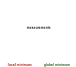
\includegraphics[width=\columnwidth]{figs/slam_local_min}
	\vspace*{-0.3in}
	\caption{An example of a local and global minimum for stereo SLAM with 10 poses and 20 landmarks from the ``Starry Night'' dataset. Ground-truth landmarks are shown as grey stars, ground-truth poses as blue frames, pose/landmark estimates are shown as frames/stars coloured red and green for local and global minima, respectively. 
	Both minima are based on the same set of measurements: stereo pixel coordinates converted to Euclidean coordinates (example shown at the top of the figure) and relative-pose measurements.
	}
	\vspace*{-0.22in}
	\label{fig:slam_local_min}
\end{figure}

\IEEEPARstart{S}{tate-estimation} is an integral component of modern robotics systems. Workhorse algorithms for state-estimation -- such as localization and simultaneous localization and mapping (SLAM) -- are now capable of estimating hundreds of thousands of states on a single processor in real time~\cite{rosenAdvancesInferenceRepresentation2021} and are far from the computational bottleneck of robotic systems. To obtain such levels of performance, these algorithms typically rely on local optimization methods (e.g., Gauss-Newton), which often exhibit super-linear convergence. In particular, SLAM has reached a high level of maturity in terms of both breadth and depth of understanding in the robotics community (see~\cite{baileySimultaneousLocalizationMapping2006} and~\cite{durrant-whyteSimultaneousLocalizationMapping2006} for a comprehensive review of SLAM).  

In recent years, we have seen a surge in interest in the use of convex, semidefinite relaxations to solve and certify the global optimality of robotic state-estimation and perception problems. 
In principle, these relaxations can be solved in polynomial time using interior-point methods\cite{vandenbergheSemidefiniteProgramming1996}. However, much of the interest in these algorithms is related to recent improvements in runtime, which have made certifiable methods more attractive for \emph{real-time} applications. These improvements have largely been brought to the robotics community by SE-Sync~\cite{rosenSESyncCertifiablyCorrect2019}, which globally solves \emph{pose-graph optimization} (PGO) -- a cornerstone of modern SLAM algorithms -- by leveraging the low-rank nature of its semidefinite program (SDP) relaxation. A series of extensions to this method have been and continue to be developed~\cite{rosenAdvancesInferenceRepresentation2021}.

Despite the success of these methods, they often rely on simplifying assumptions in order to apply these fast, low-rank algorithms. Perhaps most striking is the assumption of isotropic noise models that pervades the majority of the literature. Isotropic noise is often an unrealistic assumption for modern robotics, especially when more realistic sensor models are considered. For example,~\cite{matthiesErrorModelingStereo1987} shows that conversion of stereo pixel coordinates to Euclidean coordinates yields noise distributions that should not be modeled isotropically. When the correct model is used, the resulting maximum-likelihood optimization includes \emph{matrix} (rather than \emph{scalar}) weighting factors. 

The introduction of matrix weighting in state-estimation problems with rotations typically leads to solution methods that are more involved. For example, though a closed-form, global solution exists for scalar-weighted Wahba's problem~\cite{hornClosedformSolutionAbsolute1987, hornClosedFormSolutionAbsolute1988, wahbaLeastSquaresEstimate1965},\footnote{Wahba's problem can also be referred to as point-set registration.} when matrix weights are introduced, an iterative, local solver must be used~\cite{chengTotalLeastSquaresEstimate2019, barfootStateEstimationRobotics2017}. %Moreover, the introduction of matrix weights could lead to a cost function landscape\rev{ with more local minima}. 

We will see that introduction of matrix weighting can also have a profound effect on the convex relaxations of state-estimation problems. In many cases, problems that have tight relaxations in the scalar-weighted case have a duality gap when matrix weighting is used. These relaxations can be \emph{tightened} by adding new constraints to the SDP, but the addition of these constraints \rev{may degrade the performance of } low-rank optimization methods mentioned above. Therefore, it is paramount to understand the key causes of this loss of tightness.

In this paper, we explore the tightness of semidefinite relaxations of perception problems that have been generalized to include \emph{matrix weights} and expose the limitations that result from this generalization. \rev{In the next section, we introduce works that are closely related to this paper and establish our contributions to the field. } We then introduce the requisite background on measurement models and semidefinite relaxation methods in Section~\ref{sec:Background}. 
In Section~\ref{sec:Formulations}, we explore the impact of matrix weighting on the formulation of two key state-estimation problems in robotics: localization and SLAM.
%In particular, we show that the introduction of matrix weighting necessarily changes the formulation of the semidefinite relaxation (compared to the scalar-weighted version~\cite{holmesEfficientGlobalOptimality2023, iglesiasGlobalOptimalityPoint2020}). 
\rev{We then draw an interesting theoretical connection in Section~\ref{sec:Uncertainty} between the posterior distribution of the state estimate and dual solution (or \emph{certificate matrix}) of the semidefinite relaxation of the corresponding state estimation problem. }
In Section~\ref{sec:Simulations}, we provide an in-depth, empirical study of the effects of matrix weighting, anisotropic noise, and stereo-camera measurements on the tightness of the semidefinite relaxations \rev{defined in } Section~\ref{sec:Formulations}\rev{, drawing connections to Section~\ref{sec:Uncertainty}}. We also evaluate these relaxations on real-world dataset\rev{s}, both with and without redundant constraints\rev{,} in Section~\ref{sec:RealExp}. \rev{In particular, we show how our globally optimal solution to matrix-weighted Wahba's Problem can be used in a state-of-the-art, outdoor, stereo-localization pipeline. } Finally, Section~\ref{sec:Conclusions} presents our conclusions and ideas for future research in this area.

\section{Related Work \rev{and Contributions}}\label{sec:RelatedContrib}

There is a large range of problems for which certifiable methods already exist. To name a few, methods for robust state estimation~\cite{yangCertifiablyOptimalOutlierRobust2023,yangTEASERFastCertifiable2021}, sensor calibration~\cite{wiseCertifiablyOptimalMonocular2020,giamouConvexIterationDistanceGeometric2022}, inverse kinematics~\cite{giamouConvexIterationDistanceGeometric2022}, image segmentation~\cite{huAcceleratedInferenceMarkov2019}, pose-graph optimization~\cite{rosenSESyncCertifiablyCorrect2019}, multiple-point-set registration~\cite{chaudhuryGlobalRegistrationMultiple2015, iglesiasGlobalOptimalityPoint2020}, range-only localization~\cite{dumbgenSafeSmoothCertified2023}, planar SLAM~\cite{liuConvexOptimizationBased2012}, and range-aided SLAM~\cite{papaliaCertifiablyCorrectRangeAided2023} have all been explored. 

Many papers have considered the conditions under which a given problem \emph{can} be certified. In particular,~\cite{cifuentesLocalStabilitySemidefinite2022} shows that, under certain technical conditions, problems that have zero duality gap when unperturbed (no noise) continue to enjoy zero duality gap as long as the perturbation parameter is within a bound (i.e., the underlying problem has sufficiently low noise). For state-estimation problems, this bound is often (but not always) found empirically to be larger than noise levels encountered in practice~\cite{rosenSESyncCertifiablyCorrect2019, tianDistributedCertifiablyCorrect2021, erikssonRotationAveragingStrong2018}.

At present, certifiable perception problems can be broadly catagorized into two key groups: problems for which fast, low-rank solvers are available and problems that can be certified, but must still rely on slower SDP solution methods (e.g., interior-point methods). The next subsections provide more detail on each of these two groups.

\subsection{Fast Certifiable Perception}\label{sec:FastPerception}

More so than other problems, global optimization of \emph{rotation synchronization} has been the subject of intense study in the vision community~\cite{wilsonWhenRotationsAveraging2016, erikssonRotationAveragingStrong2018, brynteTightnessSemidefiniteRelaxations2022} and was one of the first to enjoy significant speed improvements by leveraging the \emph{low-rank} structure of the SDP relaxation via the so-called \emph{Riemannian Staircase} approach\cite{bandeiraTightnessMaximumLikelihood2017, boumalNonconvexBurerMonteiro2016}. 

Building off existing certification methods for PGO~\cite{carloneLagrangianDuality3D2015} and inspired by the success of Riemannian methods for rotation-synchronization,~\cite{rosenSESyncCertifiablyCorrect2019} introduced SE-Sync in the robotics community. SE-Sync solves PGO over $\mbox{SE}(d)$ by taking advantage of its \emph{separable} structure~\cite{khosoussiSparseSeparableSLAM2016}, marginalizing the translation variables, and using the \emph{Riemannian Staircase} to solve the resulting rotation-synchronization problem. It was later shown that this technique could be used without marginalizing translations~\cite{brialesCartanSyncFastGlobal2017} and extended to landmark-based SLAM~\cite{holmesEfficientGlobalOptimality2023}, in both cases further exploiting problem sparsity. This method was also extended to a \emph{distributed} framework in~\cite{tianDistributedCertifiablyCorrect2021} and has even been integrated into the recent Kimera-Multi pipeline~\cite{tianKimeraMultiRobustDistributed2022}. Not surprisingly, these developments have inspired further advances in the original rotational synchronization problem~\cite{dellaertShonanRotationAveraging2020}. 

Some of these methods boast runtimes that even rival state-of-the-art, local methods (e.g., Gauss-Newton-based methods~\cite{gtsam}), with the added guarantee of a global certificate~\cite{juricComparisonGraphOptimization2021, brialesCartanSyncFastGlobal2017}. An excellent review of the current state of certifiable methods is provided in~\cite{rosenAdvancesInferenceRepresentation2021}.

\subsection{Certifiable Perception with Redundant Constraints}\label{sec:RedundantConstraints}

Though SE-Sync and its derivatives are among the most performant algorithms in certifiable perception, there are several other certifiable perception problems for which low-rank methods do not result in significant performance improvements. In particular, this set of problems includes those whose semidefinite relaxations are not initially tight, but can be tightened through the addition of certain constraints. These constraints are referred as \emph{redundant constraints} because they are redundant in the original formulation of the problem, but become nonredundant (and, indeed, linearly independent) in the lifted, semidefinite relaxation.

This `tightening trick' has been known for some time in the optimization community~\cite{nesterovSemidefiniteProgrammingRelaxations2000}, and has been applied to several problems~\cite{ruizUsingRedundancyStrengthen2011, parriloSemidefiniteProgrammingRelaxations2003a}. In the computer-vision community, redundant constraints have been used to tighten generalized essential-matrix estimation~\cite{zhaoCertifiablyGloballyOptimal2020}, relative-pose estimation between cameras~\cite{garcia-salgueroTighterRelaxationRelative2022, brialesCertifiablyGloballyOptimal2018}, and registration using 3D primitives~\cite{brialesConvexGlobal3D2017}. The formulation given in the latter paper is a degenerate version of our single-pose, matrix-weighted localization formulation (see Section~\ref{sec:Localization}), in which the use of (degenerate) matrix weights is motivated by geometry rather than noise distribution. 

Interestingly, both~\cite{garcia-salgueroTighterRelaxationRelative2022} and~\cite{brialesCertifiablyGloballyOptimal2018} showed that adding redundant constraints increases the level of measurement noise for which their respective problems remain tight. In the context of robotics,~\cite{wiseCertifiablyOptimalMonocular2020} found a similar result when exploring the effect of redundant constraints on a sensor-calibration task.~\cite{yangTEASERFastCertifiable2021} introduced redundant constraints in conjunction with \emph{graduated nonconvexity}~\cite{yangGraduatedNonConvexityRobust2020} to solve \emph{robust} point-set registration globally.~\cite{yangOneRingRule2020} and~\cite{yangCertifiablyOptimalOutlierRobust2023} extended these results to several other robust perception problems by leveraging the Lasserre-moment hierarchy~\cite{henrionMomentSOSHierarchyLectures2021,lasserreGlobalOptimizationPolynomials2001}. 

This hierarchy constitutes a powerful set of theoretical tools that are guaranteed to tighten the SDP relaxation of any \emph{polynomial} optimization problem through the use of redundant variables and constraints.\footnote{Note that this class of problems encompasses almost all of the certifiable perception problems to date.} The caveat to this method is that it requires the addition of new variables and constraints -- possibly \emph{ad infinitum} -- and can quickly become intractable in practice. Techniques such as \emph{Douglas-Rachford Splitting} for certification~\cite{yangTEASERFastCertifiable2021} and the STRIDE algorithm~\cite{yangCertifiablyOptimalOutlierRobust2023} have improved runtimes when the moment hierarchy is used, but are still far from real time. 

Since certification generally depends on the number of variables and constraints used, a more efficient tightening approach is \rev{search for a small } subset of variables and constraints \rev{that is sufficient } to \rev{render } a given relaxation \emph{tight}. \rev{This reflects the approach that we take in this paper as well as in our concurrent work~\cite{dumbgenGloballyOptimalState2023a}, which searches for redundant constraints using a sampling approach.}

\rev{\subsection{Our Contributions}

The contributions of this paper are as follows:
\begin{itemize}
	\item We demonstrate that introducing matrix weights (due to anisotropic noise distributions) into existing certifiable state estimation problems can severly impact the tightness of the underlying SDP relaxation.
	\item We show that a set of redundant constraints can be used to regain tightness in these problems. To do this, we leverage results in our concurrent paper~\cite{dumbgenGloballyOptimalState2023a}, which \emph{numerically} find a redundant constraint set for a \emph{specific} problem. We interpret these numerical constraints to find algebraic constraints that can be applied to a broader range of problem instances.
	\item We establish a connection between classical probabilistic interpretations of uncertainty and the \emph{dual} or \emph{certificate} matrix and leverage this connection to further understand our empirical results and the effect of redundant constraints on tightness.
	\item We show that, while the SDP relaxation of matrix-weighted SLAM is intractable for large-scale problems, the relaxation of matrix-weighted Wahba's problem can be solved in near realtime. We apply the latter relaxation in an outdoor, stereo-localization pipeline on real-world data.
\end{itemize}

}

\section{Background Material}\label{sec:Background}

In this section, we provide the reader with some background material and notation that will be useful for the understanding of subsequent developments.

\subsection{Notation}\label{sec:Notn}
We denote matrices with bold-faced, capitalized letters, $ \bm{A} $, column vectors with bold-faced, lower-case letters, $ \bm{a} $, and scalar quantities with normal-faced font, $ a $.
Let $ \mathbb{S}^n $ denote the space of $ n $-dimensional symmetric matrices and $ \mathbb{S}_+^n $ denote the space of $ n $-dimensional symmetric positive semidefinite matrices. \rev{We equivalently write $\bm{A}\succeq\bm{0}$ whenever $\bm{A}\in\mathbb{S}_+^n$. }
Let $ \|\cdot\|_F $ denote the Frobenius norm \rev{and let $\left<\bm{A},\bm{B}\right>$ denote the Frobenius inner product. }
Let $ \diag{\bm{A}_1,\cdots,\bm{A}_N} $ denote the block-diagonal matrix with blocks corresponding to matrices $ \bm{A}_1,\cdots,\bm{A}_N $. Note that this includes the case where the $ \bm{A}_i $ are scalar (i.e., $\diag{a_1,\cdots,a_N}$, $a_i \in \mathbb{R}$).
Let $ \bm{I} $ denote the identity matrix, whose dimension will be clear from the context or otherwise specified.
Let $ \bm{0} $ denote the matrix with all-zero entries, whose dimension will be evident from the context.
Let the subscript ``$ 0 $'' denote the world frame.
Let $ \bm{t}_i^{ji} $ denote a vector from frame $ i $ to frame $ j $ expressed in frame $ i $ and $ \bm{C}_{ij} $ denote a rotation matrix that maps vectors expressed in frame $ j $ to equivalent vectors in frame $ i $.\rev{ For readability, we replace $ \bm{t}_i^{i0} $ with $ \bm{t}_i $ and $\bm{C}_{i0}$ with $\bm{C}_i$. }
Let $ \otimes $ denote the Kronecker product.
Let $ \vert S \vert $ denote the cardinality of the set $ S $.
Let $ \bm{A}^+ $ denote the Moore-Penrose pseudoinverse of a given matrix $ \bm{A} $.
Let $ \vect{\bm{A}} $ denote the \rev{column-wise } vectorization (reshape) of a given matrix $ \bm{A} $.
Let $ (\cdot)^{\times} $ denote the linear, skew-symmetric operator as defined in~\cite{barfootStateEstimationRobotics2017}.
Let $\left[N\right] = \left\{1,\cdots, N\right\} \subset \mathbb{N}$ be the set of indexing integers.

\rev{
\subsection{MAP Estimation and the Fisher Information Matrix}\label{sec:MeasModels}

In robotics, we often frame state estimation as \emph{maximum-a-posteriori} (MAP) problems, in which the optimal estimate is given by
\begin{equation}\label{opt:ConstrainedMAP}
	\bm{x}_c^* = \arg\min\limits_{\bm{x}_c\in\mathcal{M}} -\log\left(p(\bm{x}_c \vert \bm{\mathcal{D}})\right),
\end{equation}
where $p(\bm{x}_c \vert \bm{\mathcal{D}})$ is the posterior distribution function of the estimated parameter, $\bm{x}_c$, given all of the available data, $\bm{\mathcal{D}}$ and $\mathcal{M}$ characterizes the feasible set. In practice, it is common to approximate Problem \eqref{opt:ConstrainedMAP} as follows:
\begin{equation}\label{opt:UnconstrainedMAP}
	\bm{x}^*=\arg\min\limits_{\bm{x}\in\mathbb{R}^p} -\log\left(p(\bm{x} \vert \bm{\mathcal{D}})\right),
\end{equation}
where the optimization variable, $\bm{x}$, has been locally parameterized to ensure that constraints are not explicitly required.\footnote{When state estimates involve pose variables or orientations this unconstrained form can be derived using the Lie algebra vector space of $\mbox{SE}(3)$ or $\mbox{SO}(3)$.}
Optimization then proceeds by iteratively updating the local parameterization until convergence is reached.

It is often the case that we wish to ascertain not only optimal estimates, but also the uncertainty associated with these estimates. To do so, we use the \emph{Laplace approximation}, which models the posterior distribution as a Gaussian centered at the MAP estimate, $\bm{x}^*$, with inverse covariance equal to the so-called \emph{Fisher Information Matrix} (FIM), 
\begin{equation}
	\bm{\Sigma}^{-1} = -\left.\frac{\partial^2}{\partial\bm{x}^2}\log\left(p(\bm{x} \vert \bm{\mathcal{D}})\right)\right|_{\bm{x}=\bm{x}^*_u}.
\end{equation}
The FIM can be extracted directly from the Hessian of the cost function in \eqref{opt:UnconstrainedMAP} (or an approximation thereof)\footnote{When using Gauss-Newton to solve estimation problems, the Hessian is often approximated as the product of the Jacobian with its transpose.}. Its properties have been intensely studied by the robotic state-estimation community~\cite{censiAchievableAccuracyPose2009}. For instance, it is known that the minimum eigenvalues of the FIM (and their respective eigenvectors) characterize the worst-case uncertainty of an estimated parameter. 
Of particular interest here is the fact that the geometry of the measurement data (e.g., aligned uncertainty ellipsoids) can lead to degeneracy of the FIM~\cite{zhangDegeneracyOptimizationbasedState2016}.
}

% \begin{equation}
% 	\log\left(p(\bm{x} \vert \bm{\mathcal{D}})\right) \approx \eta + (\bm{x}-\bm{x}^*)^T\bm{\Sigma}^{-1}(\bm{x}-\bm{x}^*)
% \end{equation}
\subsection{Measurement Models}

In this paper, we define a \textit{directed graph}, $ \Graph = \left(\VertSet, \EdgeSet\right)$, to keep track of \rev{poses } and measurements. The vertex set $ \VertSet = \VertSetP \cup \VertSetM $ is the union of the set of vertices representing poses, $ \VertSetP =\left[N_p\right]$, and the set of vertices representing landmarks, $ \VertSetM = \left[N_m\right]$. We assume that the edge set $\EdgeSet \subset \VertSet \times \VertSet$ is partitioned as $\EdgeSet= \EdgeSet_p \cup \EdgeSet_m$, where $\EdgeSet_p\subset \VertSet_p\times \VertSet_p$ represents relative-pose measurements and $\EdgeSet_m\subset \VertSet_p\times \VertSet_m$ represents measurements of a landmark from a given pose. We assume that each edge, $(i,j)\in \EdgeSet$, is associated with an error term, $\bm{e}_{ij}$, and a matrix weight, $\bm{W}_{ij}$. The $i^{th}$ pose is a member of the Special Euclidean group:
\begin{equation}\label{eqn:pose_var}
	\mbox{SE}(3) = \left\{(\bm{C}_i, \bm{t}_i)~:~\bm{C}_i\in \mbox{SO}(3),~ \bm{t}_i\in \mathbb{R}^3\right\}.
\end{equation}
$\bm{C}_i$ represents the rotation from the world frame to the $i^{th}$ pose frame and $\bm{t}_i$ represents the translation vector from the world frame to the pose frame, expressed in the pose frame. Moreover, we will make use of the following \textit{homogeneous transformation} to represent a given robot pose:
\begin{equation}
	\bm{T}_i = \begin{bmatrix}
		\bm{C}_i & -\bm{t}_i \\ \bm{0} & 1
	\end{bmatrix}.
\end{equation}

\rev{Here, we consider MAP optimization problems over pose and landmark variables in which the cost (log-posterior) can be expressed in the following factored form\cite{barfootStateEstimationRobotics2017}}:
\begin{equation}\label{eqn:factor_graph}
	\begin{gathered}
		\rev{-\log\left(p(\bm{x} \vert \bm{\mathcal{D}})\right) = }\sum\limits_{(i,j)\in\EdgeSet_p}  J_{ij}^{p} + \sum\limits_{(i,k)\in\EdgeSet_m} J_{ik}^{m}, \\ 
		J_{ij}^{p} = \bm{e}_{ij}^T \bm{W}_{ij} \bm{e}_{ij}, ~J_{ik}^{m} = \bm{e}_{ik}^T \bm{W}_{ik} \bm{e}_{ik},
	\end{gathered}
\end{equation}
where $J_{ij}^{p}$ and $J_{ik}^{m}$ are the cost `factors', with error terms, $\bm{e}_{ij}$ and $\bm{e}_{ik}$, that depend on the problem variables and weighting matrices, $\bm{W}_{ij}$ and $\bm{W}_{ik}$. 
The exact form of these terms are discussed in the next two sections. Though our formulation here is matrix-weighted in general, we focus on \emph{anisotropic} noise for pose-landmark measurements, with relative-pose measurements remaining \emph{isotropic}.

\subsubsection{Matrix-Weighted Pose-Landmark Measurements}\label{sec:LandmarkMeas}

Each edge, $(i,k) \in \EdgeSet_m $, represents a measurement of the $k^{th}$ landmark from the $i^{th}$ pose. In robotics, the sensors that provide measurements of landmarks can often be modeled as
\begin{equation}
	\bm{d}_{ik} = \bm{g}(\bm{C}_i\bm{m}_0^{k0} - \bm{t}_i) + \bm{\epsilon}_{d,ik}, \quad \bm{\epsilon}_{d,ik} \in \mathcal{N}(\bm{0},\bm{\Sigma}_{d,ik}),
\end{equation}
where $ \bm{d}_{ik} $ represents the (raw) measurement of landmark $k$ from the $i^{th}$ pose variable, $\bm{m}_0^{k0}$ is the location of landmark $k$ in the global frame, $ \bm{g}(\cdot) $ is an invertible, smooth, nonlinear function, and $ \bm{\epsilon}_{d,ik} $ is a zero-mean error term having normal distribution with associated covariance matrix, $ \bm{\Sigma}_{d,ik} $. 

It is often desirable to convert measurements $ \bm{d}_{ik} $ to a more convenient form by inverting the measurement model (if possible) \rev{and defining the pseudo-measurement, $\tilde{\bm{m}}_i^{ki} = \bm{g}^{-1}(\bm{d}_{ik})$, with mean given by
\begin{equation*}
	\mathbb{E}(\tilde{\bm{m}}_i^{ki})=\bm{C}_i\bm{m}_0^{k0} - \bm{t}_i.
\end{equation*} 
The deviation from the mean, given by
\begin{equation}\label{eqn:lm_error_term}
	\bm{e}_{ik} = \tilde{\bm{m}}_i^{ki} - (\bm{C}_i\bm{m}_0^{k0} - \bm{t}_i),
\end{equation}
is \emph{approximately} Gaussian with zero mean and is exactly the error term for this measurement factor. } Regardless of whether $ \bm{\Sigma}_{d,ik} $ represents isotropic noise, the (linearly-transformed) covariance of $\bm{\epsilon}_{ik} $ is typically \textit{anisotropic} and is given by
\begin{equation}
	\bm{\Sigma}_{ik} = \bm{G}^T \bm{\Sigma}_{d,ik} \bm{G},
\end{equation}
where $\bm{G}$ is the Jacobian of the inverse measurement function $\bm{g}^{-1}(\cdot)$~\cite{matthiesErrorModelingStereo1987}. 
The weighting matrix in the cost factor in the MAP estimation, \eqref{eqn:factor_graph}, is then given by the inverse of the covariance matrix, $ \bm{W}_{ik} = \bm{\Sigma}^{-1}_{ik} $. Note that solving the problem under the simplifying assumption of isotropic noise -- that is, $ \bm{W}_{ik} = \sigma_{ik} \bm{I}$ with $ \sigma_k \in \mathbb{R}$ -- can be extremely detrimental to the quality of the final solution~\cite{matthiesErrorModelingStereo1987,maimoneTwoYearsVisual2007}. 

A key example of such a situation arises in a common preprocessing step of stereo-vision problems, in which pixel and disparity measurements are converted to Euclidean point measurements by inverting a known camera model.  It has been shown that this results in measurement uncertainty that is much larger in the depth direction of a given camera pose~\cite{matthiesErrorModelingStereo1987,barfootPoseEstimationUsing2011} (c.f. Figure~\ref{fig:slam_local_min}). A derivation of the inverse stereo measurement model and associated covariance is provided in Appendix~\ref{App:stereo}. 

\subsubsection{Relative-Pose Measurements}\label{sec:RelPoseMeas}

Each edge, $(i,j) \in \EdgeSet_p $, represents a relative-pose measurement, \rev{$(\tilde{\bm{C}}_{ij},\tilde{\bm{t}}_i^{ji}) \in \mbox{SE}(3)$ and its associated homogeneous transformation, $\tilde{\bm{T}}_{ij}$. } In a robotics context, these relative-pose measurements often represent IMU-based measurement information, dynamics-based prior belief propagation, or aggregate measurement data between keyframes. Similarly to~\cite{brialesCartanSyncFastGlobal2017}, we define the following relative-pose error term:
\begin{equation}\label{eqn:rel_pose_err}
	\bm{e}_{ij} = \vect{\tilde{\bm{T}}_{ij}\bm{T}_j - \bm{T}_i}.
\end{equation}
Though $\bm{W}_{ij} \succeq \bm{0} $ can be an \emph{arbitrary}, positive semidefinite matrix, we select weight matrices of the form $\bm{W}_{ij}=\diag{\sigma^2_{ij},\sigma^2_{ij},\sigma^2_{ij},\tau^2_{ij}}^{-1} \otimes \bm{I}$, since it allows us to express our cost factor as
\begin{align}\label{eqn:rel_pose_cost}
	J_{ij} &= \frac{1}{\sigma^2_{ij}} \left\Vert \tilde{\bm{C}}_{ij}\bm{C}_{j0} - \bm{C}_i\right\Vert_F^2 + \frac{1}{\tau^2_{ij}} \left\Vert \tilde{\bm{t}}^{ji}_{i} - \tilde{\bm{C}}_{ij}\bm{t}_j + \bm{t}_i \right\Vert_2^2 \nonumber\\
	&\hspace*{3pt}\rev{=\bm{e}_{ij}^T \bm{W}_{ij} \bm{e}_{ij}}.
\end{align}
where $\sigma_{ij}$ and $\tau_{ij}$ are scalar weights.\footnote{\rev{Note that these weights represent isotropic noise, although representing other distributions may be possible.}} This form of cost factor is similar to the cost used in pose-graph optimization problems (c.f.~\cite{brialesCartanSyncFastGlobal2017, rosenSESyncCertifiablyCorrect2019, holmesEfficientGlobalOptimality2023}) and is quadratic for our choice of pose variables, \eqref{eqn:pose_var}.\footnote{The choice to represent translation variables in the \emph{local} frame ($\bm{t}_i$) rather in the \emph{world} frame ($\bm{t}_0^{i0}$) \rev{allows us to keep the cost function quadratic in the variables.}}

The relative-pose error formulation also allows for the addition of \emph{prior} information about the pose variables to \eqref{eqn:factor_graph}. In this case, the relative-pose error is defined with respect to the world frame:
\begin{equation}\label{eqn:prior_pose_err}
	\bm{e}_{0j} = \vect{\tilde{\bm{T}}_{0j}\bm{T}_j - \bm{I}}.
\end{equation}

\subsection{Convex Relaxations of QCQPs}\label{sec:Relaxation}

We review the well-known procedure for deriving convex, SDP relaxations of a standard form of polynomial optimization problem.\footnote{\rev{For the sake of brevity, our introduction of these problems and concepts in this section have been stated without proof. The interested reader is referred to~\cite{cifuentesLocalStabilitySemidefinite2022,vandenbergheSemidefiniteProgramming1996} and references therein for more extensive expositions.}} This procedure was pioneered in~\cite{shorQuadraticOptimizationProblems1987} and has become the cornerstone of \textit{certifiably correct methods} in robotics and computer vision~\cite{rosenAdvancesInferenceRepresentation2021,brynteTightnessSemidefiniteRelaxations2022}. Here, we consider a \textit{homogeneous}, \textit{quadratically constrained quadratic problem} (QCQP) expressed in the following standard form:
\begin{equation}\label{opt:QCQP}
	\min\limits_{\bm{z}} \left\{ \bm{z}^T\bm{Q}\bm{z} ~\vert~ \bm{z}^T\bm{A}_i\bm{z} = 0,\forall i \in \indset{N_c}, \bm{z}^T\bm{A}_0\bm{z} = 1 \right\},
\end{equation}
where $ \bm{z}\in\mathbb{R}^n $ is the homogeneous optimization variable, $ \bm{Q}\in\mathbb{R}^{n\times n} $ represents the quadratic cost, the $ \bm{A}_i $ correspond to $ N_c $ quadratic constraints, and $ \bm{A}_0 $ corresponds to the so-called \emph{homogenizing constraint}\cite{cifuentesLocalStabilitySemidefinite2022}. Note that any problem with quadratic cost and constraints can be converted into a problem of this form~\cite{cifuentesLocalStabilitySemidefinite2022}. \rev{This includes cost functions of the form given in \eqref{eqn:factor_graph}, as long as the error terms are \emph{linear} in the optimization variables and the constraints are quadratic.}

In general, problems with quadratic equality constraints, such as QCQPs, are difficult to solve optimally because they are nonconvex~\cite{boydConvexOptimization2004}. \rev{However, a popular approach to obtaining globally optimal solutions to QCQPs involves formulating the convex, SDP  relaxation of the QCQP and subsequently showing that this relaxation is \emph{tight}. In this context, `tight' means that the relaxation and the original problem have the same optimal cost and equivalent minimizers.

It can be shown that Problem \eqref{opt:QCQP} is equivalent to the following problem~\cite{cifuentesLocalStabilitySemidefinite2022}:
\begin{equation}\label{opt:R1SDP}
	\begin{array}{rl}
		\min\limits_{\bm{X}} & \inner{\bm{Q}}{\bm{X}}\\
		s.t.&\inner{\bm{A}_{i}}{\bm{X}}= 0, \quad \forall i \in \indset{N_c}\\
		& \inner{\bm{A}_0}{\bm{X}} = 1,\\
		& \bm{X} \succeq \bm{0},\\
		& \mbox{rank}(\bm{X})=1,
	\end{array}
\end{equation}
where the last two constraints implicitly enforce the fact that $\bm{X} = \bm{x}\bm{x}^T$. In Problem~\eqref{opt:R1SDP}, we see that all the non-convexity of the problem has been relegated to a single non-convex constraint on the rank. It follows that we can find a convex relaxation of Problem~\eqref{opt:R1SDP} by removing the rank constraint: 
\begin{equation}\label{opt:SDP}
	\begin{array}{rl}
		\min\limits_{\bm{Z}} & \inner{\bm{Q}}{\bm{Z}}\\
		s.t.&\inner{\bm{A}_i}{\bm{Z}}= 0, \quad \forall i = \left[N_c\right]\\
		& \inner{\bm{A}_0}{\bm{Z}}= 1, \\
		& \bm{Z} \succeq \bm{0}.
	\end{array}
\end{equation}
}
It is well known that if the optimal solution $ \bm{Z}^* $ satisfies $ \rank{\bm{Z}^*}=1 $ then the convex relaxation is \textit{tight} to the original QCQP. \rev{Accordingly}, this condition implies that the solution can be factorized as $ \bm{Z}^* = \bm{z}^* \bm{z}^{*T} $, where $ \bm{z}^* $ is the \textit{globally optimal} solution of Problem \eqref{opt:QCQP}. 

\rev{
We note that Problems \eqref{opt:SDP} and \eqref{opt:R1SDP} have the same Lagrangian dual problem, which plays a central role in certifying global optima and can be expressed as follows:
\begin{equation}\label{opt:Dual}
	\begin{array}{rl}
		d^*=\max\limits_{\bm{H},\bm{\lambda},\rho} &-\rho \\ 
		s.t. & \bm{H}(\bm{\lambda},\rho) = \bm{Q} + \rho\bm{A}_0 +\sum\limits_{i=1}^{N_c} \lambda_i \bm{A}_i, \\
		& \bm{H}(\bm{\lambda},\rho) \succeq \bm{0},
	\end{array}
\end{equation}
where $ \rho $ and $ \bm{\lambda} = \left[\lambda_1~\cdots~\lambda_{N_c}\right]^T $ are the Lagrange multipliers corresponding to the single homogenizing and the $N_c$ quadratic constraints, respectively. 

Since Problem \eqref{opt:SDP} is convex, it has the same optimal cost as its dual, Problem \eqref{opt:Dual}.\footnote{\rev{This is a consequence of the fact that strong duality holds for convex problems under sufficient constraint qualifications\cite{boydConvexOptimization2004}. In our case, we ensure that the SDPs that we solve satisfy the Linear Independent Constraint Qualification.}} When the relaxation is tight, the optimal cost of the original QCQP, Problem \eqref{opt:QCQP}, will also be equal to the dual problem cost, a condition known as \emph{strong duality}.

In the sequel, we will also make use of the fact that strict complementarity is a \emph{generic} property of SDPs~\cite{alizadehComplementarityNondegeneracySemidefinite1997}. In our context, strict complementarity implies that
\begin{equation}
	 \mbox{rank}(\bm{Z}^*) + \mbox{rank}(\bm{H}^*)=n,
\end{equation}
where $\bm{H}^*$ represents the dual matrix at the optimal Lagrange multipliers $(\bm{\lambda}^*,\rho^*)$.\footnote{\rev{We replace $\bm{H}(\bm{\lambda},\rho)$ with $\bm{H}$ when it is clear from the context.}} If strict complementarity holds, then the relaxation is tight if and only if $\mbox{corank}(\bm{H}^*)=1$. Practically, this means that we can study tightness by considering either largest eigenvalues of $\bm{Z}^*$ or by considering the smallest eigenvalues of $\bm{H}^*$.

In practice, there are typically two ways that globally optimal solutions can be obtained for a QCQP with a tight semidefinite relaxation:
\begin{enumerate}
	\item We can solve Problem \eqref{opt:SDP} or Problem \eqref{opt:Dual} \footnote{\rev{The dual problem is solved in~\cite{brialesCartanSyncFastGlobal2017} and is then used to recover the primal solution.}} directly and extract the globally optimal solution.
	\item Given a candidate solution, $ \hat{\bm{z}} $, found via fast optimization methods, we can certify its global optimality using the dual or \emph{certificate} matrix, $\bm{H}$.
\end{enumerate}

In robotics, there is a strong preference for the latter method, since it is often much more computationally efficient than the former. State-of-the-art methods leverage low-rank SDP techniques such as that of \emph{Burer and Monteiro} (BM)~\cite{burerNonlinearProgrammingAlgorithm2003a} and the \emph{Riemannian Staircase}~\cite{rosenSESyncCertifiablyCorrect2019, boumalNonconvexBurerMonteiro2016} to solve larger problem instances in real time.

However, these methods are far less performant when redundant constraints are introduced to tighten the semidefinite relaxation.\footnote{\rev{For example, the BM approach requires a verification that the solution is a second-order critical point~\cite{boumalDeterministicGuaranteesBurerMonteiro2020a}. When redundant constraints are used, this verification step necessarily involves solving a different (non-low-rank) SDP, since they are not uniquely determined.}} \rev{As such, a key goal of this paper is to establish whether SDP relaxations of problems with matrix weights require redundant constraints and, if so, whether it is nevertheless possible to find global solutions efficiently enough for robotics applications.}

}

\section{Problem Formulations}\label{sec:Formulations}

In this section, we provide QCQP formulations for the matrix-weighted localization and SLAM problems that are considered herein. We demonstrate how the costs can be formulated in the standard quadratic form of Problem \eqref{opt:QCQP}. In the interest of brevity, we do not explicitly show the conversion of the constraints into the standard form.

\subsection{Matrix-Weighted Localization}\label{sec:Localization}

In this section, we consider localization problems with matrix weights. That is, we consider the problem of determining the estimate of a sequence of poses given matrix-weighted measurements of a set of \emph{known} landmarks. We assume that point correspondences are known and correct. 

The maximum-likelihood estimate of the poses is given by the solution to the following least-squares optimization problem:
\begin{equation}
	\label{opt:Localize}
	\begin{array}{rl}
		\min\limits_{\bm{C}_i,\bm{t}_i, \forall  i \in \VertSetP} &\sum\limits_{(i,k)\in\EdgeSet_m} \bm{e}_{ik}^T \bm{W}_{ik} \bm{e}_{ik} \\
		\mbox{s.t.} &  \rev{\bm{C}_i^T \bm{C}_i = \bm{I}}, ~\forall i = \VertSetP,\\
		& \rev{(\bm{c}_i^{1})^\times\bm{c}_i^{2} - \bm{c}_i^{3} = \bm{0},~\forall i = \VertSetP,} \\
		\mbox{where} & \bm{e}_{ik} = \tilde{\bm{m}}_i^{ki} - \bm{C}_i\bm{m}_0^{k0} + \bm{t}_i ,
	\end{array}
\end{equation}
where the variable definitions are consistent with those provided in Section~\ref{sec:MeasModels} \rev{and $\bm{c}_i^j$ denotes the $j^{th}$ column of matrix $\bm{C}_i$. It has been shown that the two constraints on the $\bm{C}_i$ in \eqref{opt:Localize} are sufficient to ensure that $\bm{C}_i\in\mbox{SO}(3)$ and can be expressed in the standard quadratic form of \eqref{opt:QCQP}~\cite{tronInclusionDeterminantConstraints}. Therefore, this problem is a QCQP since $\bm{e}_{ik}$ is \emph{linear} in $\bm{C}_i$ and $\bm{t}_i$, and the constraints are quadratic. 

It is important to note that this problem } is separable in each set of pose variables, since there are no constraints or cost elements linking any two poses. Therefore, the problem may be divided into $N_p$ subproblems, each being equivalent to the matrix-weighted version of Wahba's problem~\cite{chengTotalLeastSquaresEstimate2019, wahbaLeastSquaresEstimate1965}.\footnote{In the \rev{remainder of this paper, we refer to single-pose instances of Problem~\ref{opt:Localize} as Wahba's problem, though it is also known as registration or single-pose localization.}} In the scalar-weighted case ($ \bm{W}_{ik} = w_{ik} \bm{I} $), there is a closed-form, global solution to Wahba's problem~\cite{hornClosedFormSolutionAbsolute1988}. However, for the general matrix-weighted case, a key simplification of the cost function is no longer possible and solutions must be found iteratively with no guarantee of global optimality~\cite{barfootPoseEstimationUsing2011,barfootStateEstimationRobotics2017, crassidisSurveyNonlinearAttitude2007}. 

We collect the relevant optimization variables into a single vector, $ \bm{x}_i^T = \begin{bmatrix} \bm{c}_i^T &  \bm{t}_i^T & w \end{bmatrix} $, where $ \bm{c}_i=\vect{\bm{C}_i} $, which allows us to re-express the cost element as
\begin{equation}
	J_{ik}= \bm{x}_i^T\bm{Q}_{ik}\bm{x}_i,
\end{equation}
where the symmetric cost matrix, $\bm{Q}_{ik}$, \rev{is given in Appendix~\ref{App:LocCost}. We have also introduced a so-called \textit{homogenizing variable}, $ w $, which is subject to the \textit{homogenizing constraint}, $ w^2 = 1 $ and facilitates the reformulation of Problem \eqref{opt:Localize} into the standard form of Problem \eqref{opt:QCQP}~\cite{wiseCertifiablyOptimalMonocular2020, cifuentesLocalStabilitySemidefinite2022}. }

The full cost of Problem \eqref{opt:Localize} can be constructed by permuting and summing the matrices, $\bm{Q}_{ik}$, according to edges in $\EdgeSet_m$ and a given pose variable ordering:
\begin{equation}\label{eqn:locVar}
	\bm{z}^T = \begin{bmatrix}
		\bm{c}_{1}^T & \bm{t}_1^T & \cdots &  \bm{c}_{N_p}^T & \bm{t}_{N_p}^{T} & w
	\end{bmatrix}.
\end{equation}

\rev{In practice, it is more efficient to leverage the separability of the problem and solve for each pose via separate instances of Wahba's problem. Since each separate problem is small in dimension (13-by-13), its SDP relaxation can be solved quickly using modern interior-point solvers (see Section~\ref{sec:OutdoorLoc} for runtimes with this approach).}

The single-pose version of Problem \eqref{opt:Localize} admits a convex semidefinite relaxation that was also explored in~\cite{brialesConvexGlobal3D2017} and~\cite{olssonSolvingQuadraticallyConstrained2008} with the motivation of representing different geometric primitive measurements (lines and planes), rather than anisotropic noise. It was found that the addition of a few key redundant constraints made the relaxation tight even when noise levels were high. \rev{We corroborate these results for anisotropic noise with an extensive analysis in Section~\ref{sec:Simulations}.}

\rev{
We could potientially introduce the \textit{relative-pose measurements} described in Section~\ref{sec:RelPoseMeas} to Problem \eqref{opt:Localize} by adding the associated cost factors to the objective. The cost function given in \eqref{eqn:rel_pose_cost} is a quadratic function in the optimization variables and can be expressed in the standard homogeneous QCQP form, as shown in Appendix~\ref{App:LocCost}. However, the addition of such factors to Problem \eqref{opt:Localize} destroys the separability property, meaning that directly solving the SDP relaxation becomes much slower for reasonably sized problems (e.g., $N_p \geq 20$).
}

In Appendix~\ref{App:SDPStability}, we prove that \rev{the SDP relaxation of } Problem \eqref{opt:Localize} is always tight when measurement noise levels are low and the weighting matrices are non-degenerate.

\subsection{Matrix-Weighted Landmark-based SLAM}\label{sec:SLAM}
\rev{
In this section, we explore the effect of matrix weighting when the landmark locations, $\bm{m}_0^{k0}$, are not known \emph{a priori}. The resulting problem, known as landmark-based SLAM, is given by,

\begin{equation}
	\label{opt:landmark_SLAM}
	\hspace*{-10pt}\begin{array}{rl}
		\min\limits_{\substack{\bm{C}_i,\bm{t}_i, \bm{m}_0^{k0}\\ \forall i\in \VertSetP,\\ \forall k\in\VertSetM } } &\sum\limits_{(i,k)\in\EdgeSet_m}  \bm{e}_{ik}^T \bm{W}_{ik} \bm{e}_{ik} +\sum\limits_{(i,j)\in\EdgeSet_p}  \bm{e}_{ij}^T \bm{W}_{ij} \bm{e}_{ij}\\
		\mbox{where} & \bm{e}_{ik} = \tilde{\bm{m}}_i^{ki} - \bm{C}_{i0}\bm{m}_0^{k0} + \bm{t}_i^{i0} , \\
		&\bm{e}_{ij} = \vect{\tilde{\bm{T}}_{ij}\bm{T}_{j0} - \bm{T}_{i0}}, \\
		\mbox{s.t.} &\bm{C}_i^T \bm{C}_i = \bm{I},~\forall i \in \VertSetP.\\
		& \rev{(\bm{c}_i^{1})^\times\bm{c}_i^{2} - \bm{c}_i^{3} = \bm{0},~\forall i = \VertSetP,}.
	\end{array}
\end{equation}
Note that the cost of \eqref{opt:landmark_SLAM} includes both landmark measurements and relative-pose measurements.
In the \emph{scalar-weighted} context, the convex relaxation of an equivalent problem has already been studied and was generally found to be tight for noise levels well above those found in practical robotics scenarios~\cite{holmesEfficientGlobalOptimality2023}. 
}

\rev{On the other hand, when matrix weights are used (i.e., the noise distribution is anisotropic), the landmark-based error term \eqref{eqn:lm_error_term} } becomes \emph{quadratic} in \rev{the optimization } variables \rev{(due to the $\bm{C}_i\bm{m}_0^{k0}$ terms) and } the cost function of Problem \eqref{opt:landmark_SLAM} becomes \emph{quartic}. In the scalar-weighted case ($\bm{W}_{ik} = w_{ik}\bm{I}$), this issue is obviated by premultiplying the error terms by the inverse pose rotations to regain \rev{\emph{linearity} } of the error terms. \rev{However, preforming this operation in the matrix-weighted case will change the cost function, since $\bm{C}_i^T\bm{W}_{ik}\bm{C}_i\neq \bm{W}_{ik}$ when $\bm{W}_{ik}$ is an arbitrary positive definite matrix.\footnote{\rev{This reflects the fact that the measurement noise \emph{has an orientation} and depends on the (unknown) observation frame. This would not be an issue if all measurements were defined in a common frame, but, in practice, measurements are typically taken in the robot's frame of reference.}}} 

In order to cast Problem \eqref{opt:landmark_SLAM} as a QCQP, we follow a similar strategy to~\cite{dumbgenSafeSmoothCertified2023} and~\cite{brialesCertifiablyGloballyOptimal2018} by introducing \textit{substitution variables}, $ \bm{m}_i^{ki} $, corresponding to each available measurement, $ \tilde{\bm{m}}_i^{ki} $. These new variables must satisfy the following (quadratic) constraints:
\begin{equation}
	\bm{m}_i^{ki} = \bm{C}_i\bm{m}_0^{k0} - \bm{t}_i, \quad \forall (i,k)\in\EdgeSet_m.
\end{equation}

When the landmarks become unknown, a gauge freedom is also introduced into the problem. This has an important implication for the SDP solution; the well-known SLAM gauge freedom results in solution symmetries that cause the rank of the SDP solution to be higher than one, even when it is numerically tight~\cite{brialesCertifiablyGloballyOptimal2018}. To fix this freedom, we assume that a \emph{prior} factor term is included in the pose-graph terms for at least one pose.\footnote{As with SLAM problems in general, the pose variable in the prior, $\tilde{\bm{T}}_{j0}$, is typically used to `lock' the solution to a known pose using some exteroceptive measurement, such as GPS. However, for our purposes it can be set arbitrarily without loss of generality.}

The optimization can now be written as
\begin{equation}
	\hspace*{-5pt}
	\label{opt:SLAM}
	\begin{array}{rl} 
		\min \limits_{ \substack{\bm{C}_i,\bm{t}_i, \\ \bm{m}_0^{k0},\bm{m}_i^{ki} \\ \forall i\in \VertSetP,~ \forall k\in\VertSetM } } & \hspace*{-20pt}\sum\limits_{(i,k)\in\EdgeSet_m} \bm{e}_{ik}^T \bm{W}_{ik} \bm{e}_{ik} + \hspace*{-7pt}\sum\limits_{(i,j)\in\EdgeSet_p}  \bm{e}_{ij}^T \bm{W}_{ij} \bm{e}_{ij}\hfill \\
		\mbox{where} & \bm{e}_{ik} = \tilde{\bm{m}}_i^{ki} - \bm{m}_i^{ki},\\
		&\bm{e}_{ij} = \vect{\tilde{\bm{T}}_{ij}\bm{T}_j - \bm{T}_i},\\
		\mbox{s.t.}&\rev{\bm{C}_i^T \bm{C}_i = \bm{I},}~\forall i \in \VertSetP.\\
		& \rev{(\bm{c}_i^{1})^\times\bm{c}_i^{2} - \bm{c}_i^{3} = \bm{0},~\forall i = \VertSetP,}\\
		& \bm{m}_i^{ki} = \bm{C}_i\bm{m}_0^{k0} - \bm{t}_i, \quad \forall (i,k)\in\EdgeSet_m.
	\end{array}
\end{equation}
The pose-landmark cost elements can now be written in the standard form:
\begin{equation*}
	J_{ik}=\begin{bmatrix}
		\bm{m}_i^{ki}\\w
	\end{bmatrix}^T \begin{bmatrix}
		\bm{W}_{ik} & \rev{-}\bm{W}_{ik}\tilde{\bm{m}}_i^{ki}\\
		\rev{-}\tilde{\bm{m}}_i^{ki^T}\bm{W}_{ik} & \tilde{\bm{m}}_i^{ki^T}\bm{W}_{ik}\tilde{\bm{m}}_i^{ki}
	\end{bmatrix}\begin{bmatrix}
	\bm{m}_i^{ki}\\w
	\end{bmatrix}
\end{equation*}
The cost elements can be then permuted and summed according to our variable ordering,
\begin{multline}
	\bm{z}^T = \left[\begin{matrix}\vect{\bm{C}_{10}}^T &\bm{t}_1^{10^T} & \cdots &\vect{\bm{C}_{N_p0}}^T&\bm{t}_{N_p}^{N_p0^T} \end{matrix}\right. \\
		\left.\begin{matrix} \bm{m}_0^{k0^T} &\cdots& \bm{m}_i^{ki^T} & \cdots & w \end{matrix}\right],
\end{multline}
and we can apply the semidefinite relaxation described in~\ref{sec:Relaxation}. However, we have observed that, contrary to the scalar case, this SDP relaxation is \emph{not tight} even for low levels of noise. A similar situation occurred in~\cite{brialesCertifiablyGloballyOptimal2018} and~\cite{yangTEASERFastCertifiable2021} when substitution variables were introduced (though not when introduced in~\cite{dumbgenSafeSmoothCertified2023}).

\rev{\subsection{Tightening the Relaxations}\label{sec:Tightening}}

\rev{One of the key contributions of this paper is a concise set of redundant constraints for the problems presented above that is capable of tightening their respective relaxations. In the next sections, we empirically show that these constraints are capable of restoring relaxation tightness that is otherwise destroyed by the introduction of anisotropic noise.}

One approach that can be used to tighten this relaxation is to apply the Lasserre-moment hierarchy~\cite{henrionMomentSOSHierarchyLectures2021, lasserreGlobalOptimizationPolynomials2001}. However, this method often introduces a \emph{prohibitive} number of \rev{additional } variables and constraints to the problem~\cite{yangCertifiablyOptimalOutlierRobust2023}. 

\rev{
In constrast, we have opted to \emph{discover} a smaller set\footnote{\rev{Smaller in the sense that we do not include \emph{all} possible constraints or further ascend Lasserre's hierarchy.}} of redundant constraints that is sufficient to render each of the problems above tight for reasonable levels of noise.  To do this, we leverage a \emph{constraint learning} concept from our concurrent paper, which, \emph{for a given problem instance}, uses samples that are drawn from the feasible set to numerically find all possible constraints via a nullspace argument~\cite{dumbgenGloballyOptimalState2023a}. 

We applied the constraint learning method to small instances of the problems defined above. We then interpreted the numerical, learned constraints and cast them as equations that are commensurate with the properties of $\mbox{SO}(3)$ and could be extended to problems of any size (any number of landmarks and poses). Finally, we selected a subset of these constraints that were empirically found to lead to tightness across various problem instances. \rev{The concept of SDP stability~\cite{cifuentesLocalStabilitySemidefinite2022} provides \emph{some} guarantees that similar problems to the ones that we study will also be tight, though we cannot claim that \emph{any} instance of Problem \eqref{opt:SLAM} will be tight.}

We found that the following set of redundant constraints could be used to tighten Problem \eqref{opt:Localize}:
\begin{subequations}\label{eqn:so3_constraints}
	\begin{flalign}
		\bm{C}_i \bm{C}_i^T - \bm{I} = \bm{0},
	\end{flalign}
	\vspace*{-20pt}
	\begin{flalign}
		(\bm{C}_i^{j})^\times\bm{C}_i^{k} - \bm{C}_i^{l} = \bm{0}, ~\forall (j,k,l)\in \left\{(2,3,1), (3,1,2)\right\},
	\end{flalign}
	\vspace*{-20pt}
	\begin{flalign}
		\bm{C}_i^{j^T}\bm{C}_i^{j} - \bm{r}_{i0}^{k^T}\bm{r}_{i0}^{k} = \bm{0}, ~\forall j,k\in \left\{1,2,3\right\},
	\end{flalign}
\end{subequations}
where $\bm{C}_i^{j}$ and $\bm{r}_{i0}^{k}$ represent the $j^{th}$ column and $k^{th}$ row of $\bm{C}_i$, respectively, and $\mbox{cyclic}()$ denotes the cyclic group. Note that the first two redundant constraints were also necessary in~\cite{brialesConvexGlobal3D2017} and~\cite{wiseCertifiablyOptimalMonocular2020}. 

Moreover, our SLAM problem (Problem \eqref{opt:SLAM}) can be tightened by using \eqref{eqn:so3_constraints} in conjunction with the following constraints:
\begin{subequations}\label{eqn:slam_constraints}
	\begin{flalign}
		\bm{m}_0^{l0^T} \bm{m}_0^{k0} - (\bm{m}_i^{li}-\bm{t}_i)^T (\bm{m}_i^{ki}-\bm{t}_i) = 0,% landmark dot products
	\end{flalign}
	\vspace*{-20pt}
	\begin{flalign}
		\bm{C}_i\left(\bm{m}_0^{l0}-\bm{m}_0^{k0}\right) - \left(\bm{m}_i^{li}-\bm{m}_i^{ki}\right) = \bm{0}, % landmark to landmark vector in pose frame
	\end{flalign}
	\vspace*{-20pt}
	\begin{flalign}
	 	\left(\bm{m}_0^{l0}-\bm{m}_0^{k0}\right) - \bm{C}_i^T\left(\bm{m}_i^{li}-\bm{m}_i^{ki}\right) = \bm{0}, % landmark to landmark vector in world frame
	\end{flalign}
	\vspace*{-20pt}
	\begin{flalign}
	 	\left\Vert\bm{m}_i^{li}-\bm{m}_i^{ki}\right\Vert^2 - \left\Vert\bm{m}_j^{lj}-\bm{m}_j^{kj}\right\Vert^2 = 0, % Landmark differences in different frames
	\end{flalign}
	\vspace*{-20pt}
	\begin{flalign}
	 	\left(\bm{m}_0^{l0}-\bm{m}_0^{k0}\right)^{\times} \bm{C}_i - \bm{C}_i \left(\bm{m}_0^{l0}-\bm{m}_0^{k0}\right)^{\times} =\bm{0}, % Adjoint Equation
	\end{flalign}
	\vspace*{-20pt}
	\begin{flalign}
		\bm{t}_i - \left(\frac{1}{N_i}\sum_{i=1}^{N_i}\bm{C}_i \bm{m}^{k0}_0 - \bm{m}^{ki}_i\right) = \bm{0}, % average pose
	\end{flalign}
	\vspace*{-10pt}
	\begin{flalign*}
		\hspace*{50pt}\forall i,j,l,k~ \mbox{s.t.}~ \left\{(i,l),(i,k),(j,l),(j,k)\right\}\subset\EdgeSet_m.\nonumber
	\end{flalign*}
\end{subequations}

Despite the fact that these constraints successfully tighten our problems for practical noise levels, the presence of redundant constraints prohibits the use of fast certification methods as mentioned above, meaning that interior-point methods must be used to certify or solve the relaxation. Therefore, it is very important to characterize the noise regime for which the convex relaxation of Problem \eqref{opt:landmark_SLAM} is still tight, which is the subject of Section~\ref{sec:NoiseAnalysis}.

Due to the large number of variables and constraints that must be introduced, the problem sizes that can be solved using this method are still small. This may be mitigated by exploiting the sparsity of the problem, but this remains as future work. One notable exception is the localization problem without relative-pose measurements, which is still reasonably tractable due to the separability of the problem. 
}

\rev{
\section{Estimation Uncertainty and the Dual Certificate}\label{sec:Uncertainty}

In this section, we present a set of theoretical results that allows us to extend intuitions about uncertainty in state estimation to tightness of SDP relaxations. We establish a connection between the dual solution of the SDP relaxation (specifically the certificate matrix, $\bm{H}$) and the Fisher Information Matrix. 

The following Lemma relates the dual SDP solution and the Laplace approximation of an equivalent (local) unconstrained problem of the form \eqref{opt:UnconstrainedMAP}. 

\begin{lemma}\label{thm:FisherInfo}
	Suppose a given MAP estimation problem can be equivalently formulated as either a standard-form, homogenized QCQP \eqref{opt:QCQP} or as an unconstrained optimization as in \eqref{opt:UnconstrainedMAP}. Let $\bm{z}^*$ and $\bm{x}^*$ be the (global) optima of these formulations, respectively. Given a neighborhood, $\mathcal{U} \subseteq \mathbb{R}^p$, containing $\bm{x}^*$, let $\bm{\ell}: \mathbb{R}^p \mapsto \mathbb{R}^n$ be a \emph{smooth, injective} map on $\mathcal{U}$, such that its image is in the feasible set of \eqref{opt:QCQP}. Moreover, let the respective objective functions be equal under the map in the neighborhood $\mathcal{U}$. That is,
	\begin{equation}
		-\log\left(p(\bm{x} \vert \bm{\mathcal{D}})\right) = \bm{z}^T \bm{Q} \bm{z},
	\end{equation}
	for all $(\bm{x}, \bm{z})$ such that $\bm{z}=\bm{\ell}(\bm{x})$ and $\bm{x} \in \mathcal{U}$. Then the FIM of $p(\bm{x} \vert \bm{\mathcal{D}})$ is given by
	\begin{equation}\label{eqn:FIM_H}
		\bm{\Sigma}^{-1}= \bm{L}^T \bm{H}\bm{L},
	\end{equation}
	where $\bm{H}$ is the dual certificate matrix at the solution and $\bm{L}$ is the Jacobian of the $\bm{\ell}(\bm{x})$ at the solution, $\bm{L} = \frac{d}{d\bm{x}}\bm{\ell}(\bm{x})\vert_{\bm{x}=\bm{x}^*}$. 
\end{lemma}
We defer the proof of this Lemma to Appendix~\ref{App:lemma1Proof}. Intuitively, the Lemma uses the fact that the local curvature of the two problems are equal on the feasible set to establish a connection between the FIM and the certificate matrix. 

Note that the existence of the mapping, $\bm{\ell}$, is not restrictive in our context. In fact, since the feasible set of the problems in this paper are smooth manifolds, this mapping can be interpreted as the \emph{inverse coordinate chart} from differential geometry.  We provide examples of how to construct such a mapping for Wahba's problem in Appendix~\ref{App:UncEx}.

One implication of this Lemma is that the certificate matrix can be interpreted as an information matrix in the higher-dimensional, SDP space.
It also provides a method to extract posterior covariance matrices from a given SDP solution. We use Lemma~\ref{thm:FisherInfo} in the following proposition, which will be important to our subsequent analysis:
\begin{proposition}\label{thm:eig_bounds}
	Assume that the setting of Lemma~\ref{thm:FisherInfo} holds. Then the following relation holds:
	\begin{equation}
		\sigma(\bar{\bm{H}})  \leq \frac{\sigma(\bm{\Sigma}^{-1})}{\sigma(\bm{L})^2}, 
	\end{equation}
	where $\sigma(\cdot)$ denotes the smallest singular value (or eigenvalue for PSD matrices) and $\bar{\bm{H}}$ is the certificate matrix with row and column corresponding to the homogenization variable removed.
\end{proposition}

The proof of this proposition is given in Appendix \ref{App:prop1Proof}.
Note that the $\sigma(\bm{L})^2$ is a scaling that accounts for the choice of parameterization for the unconstrained optimization. However, for common choices of Lie algebra vector spaces, the eigenvalues of $\bm{L}$ are bounded between one and two.

This proposition implies that tightness of the SDP relaxation is eroded as the posterior distribution becomes more uncertain. To see why this is true, 
note that if there is large uncertainty in the posterior estimate, then $\sigma(\bm{\Sigma}^{-1})$ decreases. Owing to Theorem~\ref{thm:eig_bounds}, we see that the upper bound on $\sigma(\bar{\bm{H}})$ also decreases, pushing $\bar{\bm{H}}$ closer to being rank deficient. If $\bar{\bm{H}}$ actually becomes rank deficient then $\mbox{corank}(\bm{H})>1$, and, as long as strict complementarity holds,\footnote{\rev{We acknowledge the fact that strict complementarity does not \emph{always} hold for SDPs, but have empirically observed that it holds for the problems we consider herein.}} $\mbox{rank}(\bm{X}^*)>1$ and the problem becomes nontight.

In our subsequent analyses, we will use the implication above to understand the cause of loss of relaxation tightness when anisotropic noise is introduced to our state estimation problems. 
}

\section{Simulated Experiments}\label{sec:Simulations}

It is known that the tightness of SDP relaxations of least-squares perception problems depends on the level of noise in the measurements~\cite{brialesConvexGlobal3D2017, rosenSESyncCertifiablyCorrect2019, cifuentesLocalStabilitySemidefinite2022}. For the case of rotational averaging, tightness of the relaxation has been linked to the magnitude of \textit{residual uncertainty} of pose estimates~\cite{erikssonRotationAveragingStrong2018}.

In this section, we empirically explore the effect that introducing anisotropic noise and matrix weights have on localization and SLAM. Our study is strongly motivated by stereo-camera noise models, but not limited thereto. 
All of the results in this and the next section were generated using MOSEK's interior-point, SDP solver~\cite{mosek}.

It is common in the literature report average rank when assessing tightness of the SDP relaxation, but we find that the \rev{eigenvalue } ratio \rev{(ER) of the optimal solution } -- that is, the ratio between the first and second \rev{eigen}values -- is a more informative metric for tightness. Generally, $\mbox{\rev{ER}}\geq 10^6$ is an appropriate indicator that an SDP relaxation is rank-one and therefore tight. In the subsequent analysis, we use this metric as the main criterion for tightness. 

As mentioned above, when measurements are based on a stereo-camera model, the uncertainty ellipsoids in Euclidean space become elongated. This elongation occurs along rays extending from the camera focal point and depends quadratically on the distance to the measured point. To capture this elongation, we define the \textit{anisotropicity} of a measurement as the square root of the conditioning number of the noise covariance matrix (i.e., square root of ratio of maximum to minimum eigenvalues). Figure~\ref{fig:ellipsoid_align}(a) presents a visualization of the shape of an uncertainty ellipsoid as anisotropicity changes.

\rev{All of the studies in this section have the same general format. Landmark locations were randomly generated from a uniform distribution within a bounding cube of a given size and distance relative to the pose/camera frame. Unless otherwise specified, the default values for distance and bounding cube length are 3 m and 1 m, respectively. 

We searched for sets of parameters that have tight relaxations through a variety of analyses. For each analysis, the parameter space was sampled using a 30-by-30 grid in logspace across the ranges shown in the figures. For each point in the parameter space, the SDP was solved for 100 random landmark and pose geometries generated using random seeds that were consistent across parameter points. For each point in parameter space, the minimum ER was found across all trials and boundaries were plotted along the parameter values at which the minimum ER dropped below $1\times10^{-6}$.\footnote{Note that in reality, the raw contours are quite noisy. For convenience to the reader, we first smooth the minimum \rev{ER } values with a median filter, then plot the contours. The smoothing method is reviewed Appendix~\ref{App:Smoothing}.}}

\rev{\subsection{Anisotropic Noise in Wahba's Problem}\label{sec:NoiseAnalysis}
}
In this section, we directly control the level and alignment of measurement noise anisotropicity (i.e., uncertainty ellipoid size and shape) and observe their effect on the tightness of Wahba's problem. 

\rev{\subsubsection{Aligned Uncertainty Ellipsoids}}

We first study the effect of \rev{anisotropic noise } on Wahba's problem and consider the simplified case in which all of the error ellipsoids are aligned. \rev{The alignment of the ellipsoids causes the uncertainty to be concentrated in a single direction leading to high posterior uncertainty in that direction~\cite{zhangDegeneracyOptimizationbasedState2016}. This case is of interest since our analysis in Section~\ref{sec:Uncertainty} suggests that there is a connection between high posterior uncertainty and loss of tightness. }

Figure~\ref{fig:ellipsoid_align} shows the boundary between tight and nontight SDP relaxations for this problem as the standard deviation (STD) \rev{of the noise}, anisotropicity \rev{of the noise } and number of landmarks are varied. \rev{The problem setup is shown in Figure~\ref{fig:ellipsoid_align}(b), while Figure~\ref{fig:ellipsoid_align}(a) demonstrates the effect of increasing anisotropicity on the uncertainty ellipsoid.}

\rev{Figure~\ref{fig:ellipsoid_align} (c) and (d) show the parameter-space regions that have tight relaxations without and with (respectively) the redundant constraints in \eqref{eqn:so3_constraints}. For the case without redundant constraints}, we see that when anisotropicity is close to one (i.e., nearly isotropic), the noise level that yields tight relaxations is high even for low numbers of landmarks. These results are consistent with previous results for isotropic noise~\cite{holmesEfficientGlobalOptimality2023}. Increasing the number of landmarks generally improves tightness for a given noise level. We also see that for any given level of noise, increasing anisotropicity eventually results in a loss of tightness. 

\rev{
It is clear that the redundant constraints effectively make the problem tight across almost all parameters studied. The effect of the redundant constraints as well as the relationship between tightness, the certificate matrix and the FIM are explored in greater depth in Figure~\ref{fig:cert_eig_study}. This figure shows heatmaps for the 50 landmark case of Figure~\ref{fig:ellipsoid_align}, without and with redundant constraints, across three metrics: the solution ER (subplots (a) and (b)), second smallest eigenvalue of the certificate matrix (subplots (c) and (d)), and the minimum eigenvalue of the FIM ((e) and (f)). The FIM was calculated using \eqref{eqn:FIM_H} with the mapping $\bm{L}$ as defined in  Appendix~\ref{App:UncEx}. 

A number of key observations can be drawn. First, we note that the tightness boundary in (a) (magenta line)\footnote{Note that this line is the same as the same boundary as shown in Figure~\ref{fig:ellipsoid_align}(c).} coincides almost exactly with the drop in the certificate matrix eigenvalue in (c), as expected.\footnote{\rev{This actually demonstrates that strict complementarity mostly holds for this problem, since a drop in rank of the certificate is exactly complemented by an increase in rank of the solution matrix.}} 

Second, by comparing (c), (d) and (f), we see that the introduction of redundant constraints increases the certificate eigenvalue to close to the FIM upper bound (though it does not quite attain it). It is interesting to note that the bound in Theorem~\ref{thm:eig_bounds} is quite loose without redundant constraints. 

Finally, we note that the FIM changes very little when redundant constraints are introduced. This is expected, since the FIM for a given problem should not depend on the redundant constraints. We posit that slight differences that we observe between plots (e) and (f) are numerical in nature. 

}

\begin{figure}[!t]
	\centering
	%\vspace*{-0.05in}
	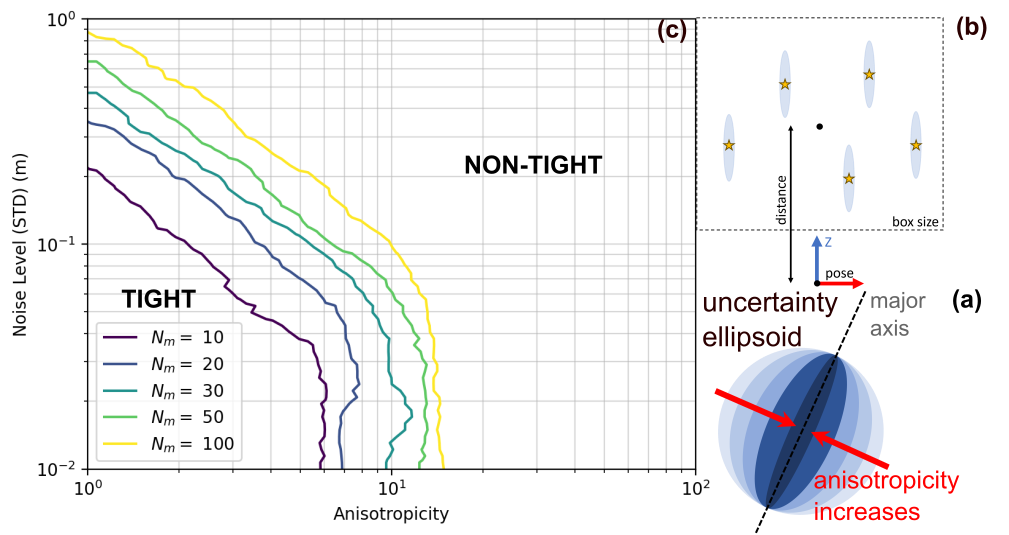
\includegraphics[width=\columnwidth]{figs/elliposoid_align_fig.png}
	%\vspace*{-0.3in}
	\caption{Investigation of the effect of anisotropicity on tightness of semidefinite relaxations for Wahba's problem.  Subplot (a) shows how varying anisotropicity affects the uncertainty ellipsoid. Subplot (b) shows the problem setup, with ellipsoids aligned to the $z$-axis of the pose. Subplot (c) shows the tightness boundary for varying numbers of landmarks. Anisotropicity decreases the tightness boundary while increasing number of observed landmarks increases the boundary.}
	%\vspace*{-0.22in}
	\label{fig:ellipsoid_align}
\end{figure}


\begin{figure}[!t]
	\centering
	\includegraphics[width=\columnwidth]{figs/cert_eig_study.png}
	\caption{Extended study of the results in Figure~\ref{fig:ellipsoid_align} for the 50 landmark case. Heatmaps represent the value of each metric specified in the left-most column, both without (left column) and with (right column) redundant constraints. The presence of the redundant constraints pushes the second certificate eigenvalue closer to the minimum eigenvalue of the FIM, leading to a relaxation that is tight over a larger region of the parameter space. Note that there is a significant heatmap scale difference between (a) and (b) and between (c) and (d). }
	\label{fig:cert_eig_study}
\end{figure}

\rev{
\subsubsection{Misaligned Uncertainty Ellipsoids}\label{sec:SimMisalign}

We now consider the effect of varying the \emph{orientation} of the uncertainty ellipsoids. In classical state estimation, it is known that high-quality estimates can still be obtained when measurements have high uncertainty in a particular direction, as long as these directions are not aligned. Leveraging our insight from Section~\ref{sec:Uncertainty}, we expect to see a similar trend with the tightness of the SDP relaxation.
 
Figure~\ref{fig:wahba_axis_bnd} demonstrates two experiments that vary uncertainty ellipsoid orientation in the same setting as for Figure~\ref{fig:ellipsoid_align}. \rev{Figure~\ref{fig:wahba_axis_bnd}(a) } shows results for random rotational perturbation of ellipsoid alignment while \rev{Figure~\ref{fig:wahba_axis_bnd}(b) } shows the effect of the `fanning out' of ray-aligned ellipsoids as the size of the landmark bounding cube is increased. 
}
\begin{figure}[!b]
	\centering
	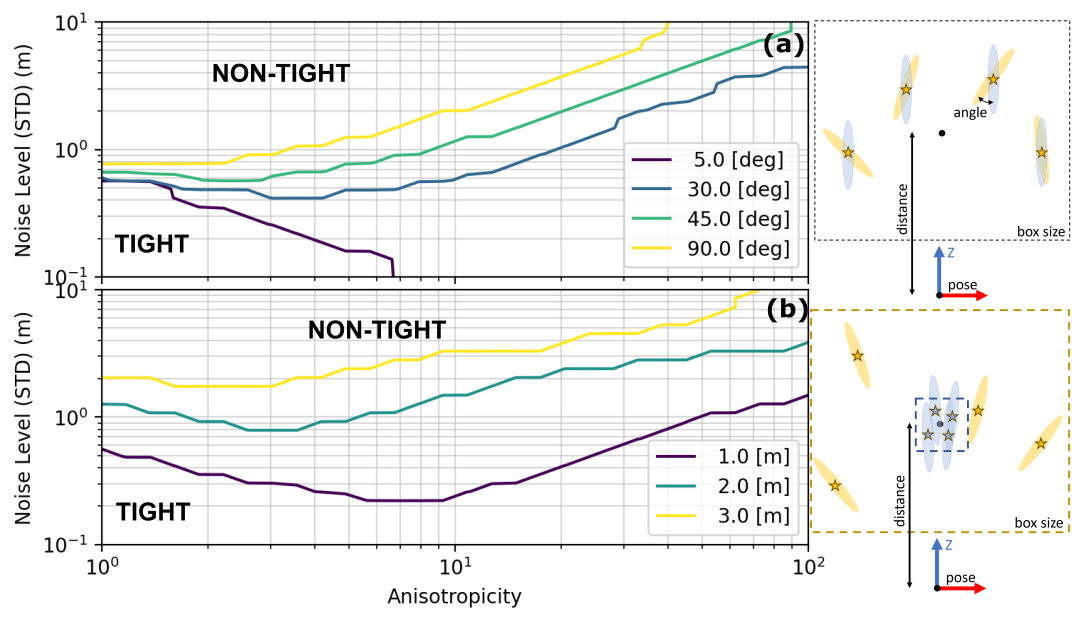
\includegraphics[width=\columnwidth]{figs/ellipsoid_study}
	\caption{Tightness boundary for Wahba's problem instance with 20 landmarks observed. In (a), axes of maximum uncertainty are aligned to pose $z$-axis then perturbed by random angles with different standard deviations (see legend). In (b), maximum uncertainty axis is aligned to pose-landmark ray and size of the bounding box on the landmarks is varied (size in legend). In both cases, increased variation of uncertainty ellipsoid axes yields tighter relaxations as anisotropicity increases. Additionally, in both cases, the entire parameter space was tight when redundant constraints were used.}
	\label{fig:wahba_axis_bnd}
\end{figure}

\rev{
In both cases, the trends coincide with our expectation: when the ellipsoids are \textit{aligned}, uncertainty is concentrated on a single axis and tightness is lost at a lower noise level. On the other hand, when the ellipsoids are highly \textit{misaligned}, uncertainty is not concentrated and the problems are tighter for much higher noise levels. 

Another interesting trend that we observe is that in most cases the tightness boundary begins to increase along the noise-level axis as anisotropicity increases. Because the axes are misaligned, high uncertainty of one measurement along a given direction, can be complemented by low certainty of a different measurement along the same direction. We posit that this causes the posterior uncertainty (and hence tightness) to be dominated by ellipsoid minor-axis uncertainty, which decreases as anistropicity increases. 

We did not include the results for Figure~\ref{fig:wahba_axis_bnd} with redundant constraints because all of the studied parameter values were tight. 
}

\rev{\subsection{Wahba's Problem with Stereo-Camera Noise Model}\label{sec:SimWahbaStereo}

Levaraging our understanding from the previous section, we now turn our attention to Wahba's problem with measurements obtained from a less idealized, stereo-camera-based noise model. Both the measurement noise level and anisotropicity depend strongly on the distance between a pose and the observed landmarks (see \eqref{eqn:stereo_jac} at the end of Appendix~\ref{App:stereo}). Additionally, posterior uncertainty in stereo-camera-based localization depends on the `spread' of the landmarks being measured. As such, our experiments in this section explore tightness as a function of the distance to and size of the landmark bounding cube (see Figure~\ref{fig:stereo_redun}(a) for problem setup). The measurements and their associated covariances are drawn from the stereo-camera model with parameters given in Table~\ref{tbl:cam_params}.

Figure~\ref{fig:stereo_redun} (b) and (c) show the tightness boundaries for this setup without and with the redundant constraints given in \eqref{eqn:so3_constraints}. 
The figure shows results for Wahba's problem with different numbers of landmarks. As expected, the level of noise for which the relaxation is tight is inversely proportional to the average distance between pose and landmarks. On the other hand, increasing the spread (bounding cube) of the landmarks increases the tightness boundary, which is consistent with our previous observations for the ellipsoid model. 

Note that for this camera model, Wahba's problem is not very tight without redundant constraints: the tightness boundary when 50 landmarks are constrained to a unit cube is a range of approximately 2 m for a 0.24 m baseline camera. In constrast, the problem becomes considerably tighter when the redundant constraints are employed, with the maximum range of 100 m. This is a clear indication that redundant constraints are required for practical robotics applications. As we will see in Section~\ref{sec:OutdoorLoc}, it is feasible to use redundant constraints in this problem, while still maintaining computational efficiency. 
}

\begin{figure}[!t]
	\centering
	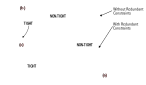
\includegraphics[width=\columnwidth]{figs/stereo_redun_study}
	\caption{Investigation of tightness boundaries for Wahba's problem with a stereo-camera model without and with redundant constraints. A diagram of experiment setup is shown in (a). (b) shows the effect of increasing the number of landmarks without redundant constraints. (c) shows the boundaries for the same model and scenario, but with redundant constraints included. Note that the sampled distance parameter ranges are different between (a) and (b).}
	\label{fig:stereo_redun}
\end{figure}

\subsection{SLAM with Stereo-Camera Noise Model}\label{sec:SimStereoSLAM}

In Figure~\ref{fig:stereo_slam_redun}, tightness boundaries are shown for the SLAM problem with redundant constraints using the same simulation setup as in Figure~\ref{fig:stereo_redun}. We do not show the results for SLAM without redundant constraints because none of the cases that we studied were found to be tight. Again, increasing the number of landmarks expands the tightness boundary, but curiously, the spread of the landmarks (indicated by the bounding box) seems to have little-to-no effect on tightness.

\rev{
We note that although the redundant constraints are capable of tightening the problem, the runtime of these problems is prohibitive for real-time application. This is due to the size of the problem: for a single pose problem with 20 landmarks the dimension of the SDP variable is $133$ and the number of constraints required is $3343$. These numbers also increase quite rapidly as the number of poses increases. 
}
\begin{figure}[!t]
	\centering
	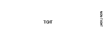
\includegraphics[width=\columnwidth]{figs/slam_lms_redun}
	\caption{Investigation of tightness boundaries for a single-pose SLAM problem with a stereo-camera model with redundant constraints. A diagram of the scenario is shown in Figure~\ref{fig:stereo_redun} (a). Boundaries are not shown when redundant constraints are not used because the problem was not tight across all of the parameters studied here.}
	\label{fig:stereo_slam_redun}
\end{figure}

\rev{
\section{Real-World Experiments}\label{sec:RealExp}
\subsection{Outdoor Stereo Localization}\label{sec:OutdoorLoc}

In the preceding sections, we have mentioned the fact that since matrix-weighted Wahba's problem has a small number of variables and constraints ($13$ and$31$, respectively), it is still feasible to use the SDP relaxation for post processing or even real-time applications. In this section, we apply our relaxation of matrix-weighted Wahba's problem (Problem \eqref{opt:Localize}) in the stereo-localization pipeline introduced in~\cite{gridsethKeepingEyeThings2022}, which uses a neural network to detect a set of features that are robust to seasonal and lighting conditions.

\subsubsection{Stereo-Localization Pipeline}

The full pipeline can be seen in Figure~\ref{fig:inthedark}(d). A neural network is used to detect features and provide descriptors for subsequent data association. The features are converted from 2D stereo keypoints to 3D keypoints, which are then used to estimate relative poses between keyframe stereo images in a stored map and corresponding stereo images from a `live run'. In~\cite{gridsethKeepingEyeThings2022}, the pose is estimated via random sample consensus followed by pose refinement with a scalar-weighted Singular Value Decomposition (SVD)\footnote{\rev{See~\cite{umeyamaLeastSquaresEstimationTransformation1991} for more details on this method.}} approach. 
}
\rev{
\subsubsection{Modifications to Pose Estimation}

We replace the pose refinement block with a matrix-weighted optimization (i.e., Wahba's problem). A stereo-camera model is used to compute the inverse covariances of the 3D keypoint measurements (see Section~\ref{App:stereo} for details), which are then used as the matrix weights. Since the pipeline does not make use of relative-pose measurements (i.e., IMU data), each pose can be solved separately. 

We solved the matrix-weighted pose-refinement optimization with both a local solver and global solver. The local optimization was performed using a Gauss-Newton solver over the $\mbox{SE}(3)$ Lie group in an off-the-shelf framework called Theseus~\cite{pinedaTheseusLibraryDifferentiable2022}. Tolerances (relative and absolute) were set to $1\times10^{-10}$ with 200 as the maximum number of iterations. The maximum number of iterations recorded was 160. Theseus was initialized using the best pose estimate from RANSAC, as is common in practice.

The problem was solved globally via the SDP relaxation of Problem \eqref{opt:Localize} \emph{with} the redundant constraints given in \eqref{eqn:so3_constraints}. The cost matrix was computed as shown in Section~\ref{App:LocCost}. For each pose, we used CVXPY~\cite{diamondCVXPYPythonEmbeddedModeling} with Mosek~\cite{mosek} to solve the SDP. The solution was extracted by selecting the column corresponding to the homogenizing variable in the solution matrix. The relevant interior-point tolerances for Mosek were also set to $1\times10^{-10}$ with the maximum iterations set to 1000 (though the number of iterations did not exceed 30).

All approaches were implemented in PyTorch. Note that the entire pipeline up to the pose refinement step (including RANSAC with SVD to find inliers) was identical for both solvers pipelines. On average, approximately 542 inlier 3D measurements were returned by RANSAC for the refinement step.  

\subsubsection{Dataset and Results}
\color{red}

\begin{figure}[]
	\centering
	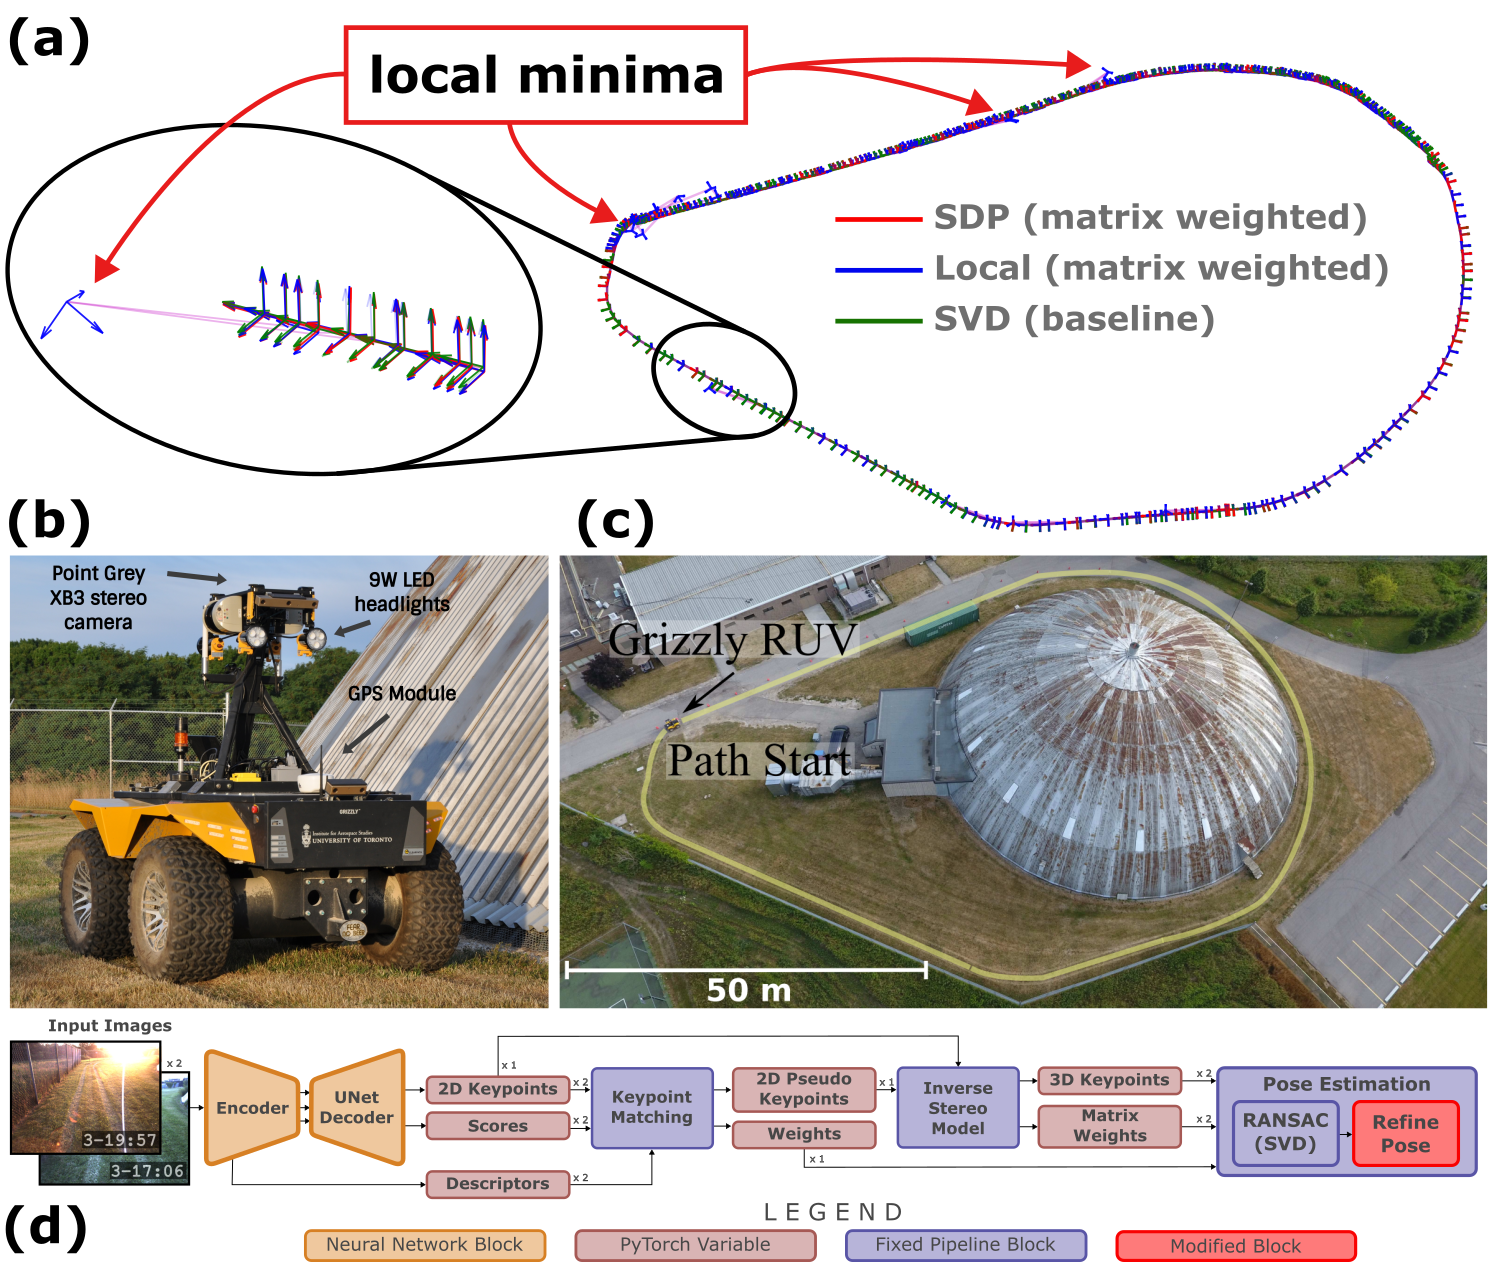
\includegraphics[width=\columnwidth]{figs/in-the-dark-traj.png}
	\caption{Overview of the setup and results of the outdoor stereo localization experiment introduced in Section~\ref{sec:OutdoorLoc} (map run: 2, live run: 16). (a) shows the estimated trajectory for all three methods and highlights the local minima that appear when using the Local method. (b) shows the robot (Grizzly RUV) and camera (Point Grey XB3) that were used. (c) shows an aerial view of the localization track and (d) shows the stereo-localization pipeline (with modified blocks in \color{red}{red}).}
	\label{fig:inthedark}
\end{figure}

We tested the pipeline on runs 2, 11, 16, 17, 23, 28, and 35 from the `In-the-Dark' dataset, which was used for training and testing in~\cite{gridsethKeepingEyeThings2022}.\footnote{\rev{Dataset is available at \url{http://asrl.utias.utoronto.ca/datasets/2020-vtr-dataset/}. The selected runs correspond to the hold-out test runs from~\cite{gridsethKeepingEyeThings2022}.}} The number of poses in each run varies, ranging between 886 and 3634, but the path taken in all runs is shown in Figure~\ref{fig:inthedark} (c). 

We localize between all pairs of the seven runs (21 localizations total). Each run can be used as either the `map' or the `live' run since all are equiped with ground truth. Localization was performed for the Baseline (SVD), Local (Theseus), and Global (SDP) solvers by running the pipeline with each on an NVIDIA Tesla V100 DGXS GPU with a Intel Xeon 2.20GHz CPU. We present the aggregate results of the analysis in terms of average time per pose, longitudinal root-mean-square error (RMSE), latitudinal RMSE, and heading RMSE for each of the pipelines in Table~\ref{tbl:inthedark}. A full set of results is provided in Appendix~\ref{App:inthedarkExt}.

It is immediately clear that the Local solver performs significantly worse than than the Baseline and Global methods. Further investigation revealed that this was because, for several poses throughout the runs, the Local solver converged to egregious local minima. An example of such a minimum can be seen in Figure~\ref{fig:inthedark}(a). As such, we have added a `filtered' row to Table~\ref{tbl:inthedark}, which provides the Local solver results when pose estimates with heading error larger than 3 deg are removed. Even when filtered, the Local solver still has the largest RMSE values, possibly due to less salient local minima.

It is interesting that the (scalar-weighted) Baseline approach outperforms the (matrix-weighted) approaches in terms of RMSE and compute time. However, we note that the `ground truth' trajectories for each run were computed by minimizing a reprojection-based cost (see~\cite{patonBridgingAppearanceGap2016a}) and are subject to additional error, which is likely on the order of the difference between the Baseline and Global solvers ($\leq0.005$ m and $\leq0.05$ deg). Further, the fact that the neural network was trained \emph{using} the Baseline approach likely contributes to the performance difference.

Finally, we call attention to the fact that, in terms of speed, the Global SDP approach was approximately as fast as the Local approach and both of these approaches ran only about 2.3 times slower than the (closed-form) Baseline solution. Given the speed (8.19 Hz) and accuracy of the SDP solver, the authors argue that it could be used for online estimation, especially if implemented in a more performant language than Python (such as C++).
}
\begin{table}
	\label{tbl:inthedark}
	\centering
	\color{red}
	\caption{Aggregate Results Across Runs for In-The-Dark Dataset}
	\begin{tblr}{lcrrrrr}
		\hline
		Pipeline & Weights & {Avg. Time\\Per Pose} & {Long.\\RMSE\\(m)} &  {Lat.\\RMSE\\(m)} &   {Head.\\RMSE\\(deg)} \\
		\hline
		Baseline     &  scalar  &    0.055 & 0.025 & 0.013 & 0.249 \\
		Global       &  matrix  &    0.121 & 0.033 & 0.021 & 0.335 \\
		Local        &  matrix  &    0.118 & 0.175 & 0.153 & 5.415 \\
		{Local\\(filtered)}& matrix &    0.118 & 0.037 & 0.035 & 0.598 \\
		\hline
	\end{tblr}
\end{table}
\rev{
\subsection{Stereo SLAM in a Controlled Environment}\label{sec:stereoslam_starry}
}

In this section, we test matrix-weighted SLAM on the `Starry Night' dataset~\cite{barfoot2011state}, which provides stereo-camera measurements of a set of known landmark locations (with known data association). \rev{The parameters of the stereo-camera model are shown in Table~\ref{tbl:cam_params}, with parameter symbols consistent with those described in Appendix~\ref{App:stereo}.}

\begin{table}[H]
	\color{red}
	\caption{Ground-Truth Camera Parameters}\label{tbl:cam_params}
	\centering
    \begin{tabular}{ |l|c|c|c|c|c|c|c| }
    \hline
    Parameter& $b $ & $f_u$ & $f_v$ & $c_u$ & $c_v$ & $\sigma_u$ &  $\sigma_v$ \\ \hline
	Units& m & $\frac{\mbox{pix}}{\mbox{m}}$ & $\frac{\mbox{pix}}{\mbox{m}}$ & pix & pix & pix & pix \\
	\hline
    Values & 0.24 & 484.5  & 484.5  & 0.0  &  0.0 & 6.32 &  11.45 \\
	\hline
    \end{tabular} 
\end{table}
\rev{
To assess tightness of matrix-weighted SLAM with stereo-image measurements, we randomly select 10 poses from the dataset and solve the SDP relaxation with and without redundant constraints. } We add relative-pose measurements between subsequent poses based on the ground-truth data and perturb these measurements by a controlled amount of (isotropic) noise allowing to assess the effect of these additional measurements. All measurements and matrix-weights were defined as explained in Section~\ref{sec:Background} and the related sections of the Appendix.

The results are shown in Figure~\ref{fig:d3_slam_box}. \rev{At all times, the distance between the pose and the landmarks is within 1.75 m. } Without redundant constraints, the problem is not tight across the noise levels considered. On the other hand, with redundant constraints, the problem remains tight until the relative-pose measurement noise exceeds approximately 0.06 m and 0.06 rad, reflecting tightness up to a reasonable level of noise. 

\begin{figure}[!b]
	\centering
	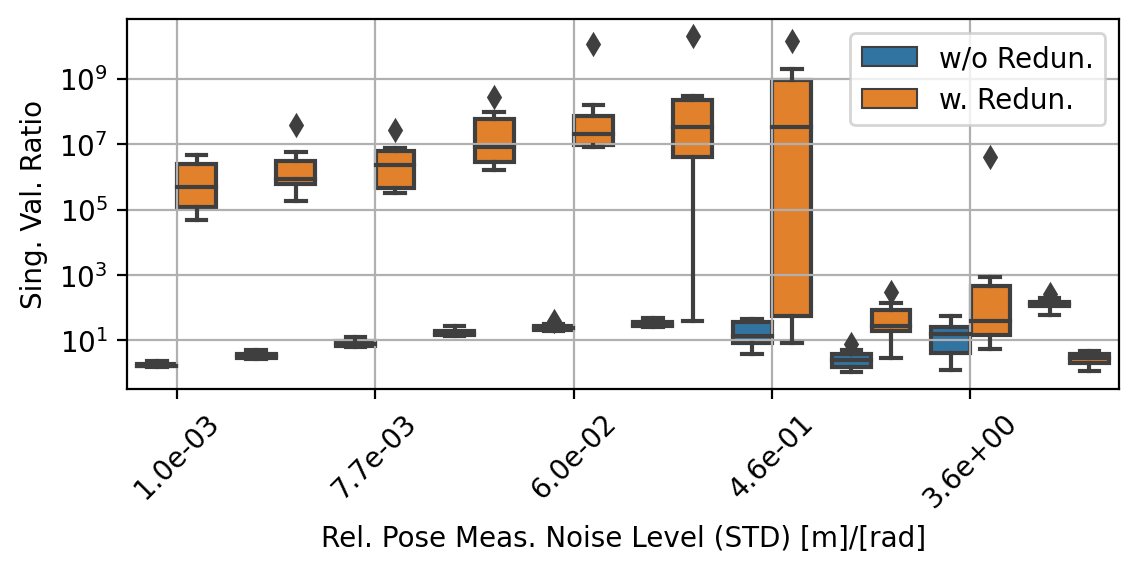
\includegraphics[width=\columnwidth]{figs/d3_slam_redun_box}
	\caption{\rev{ER } results with and without redundant constraints for SLAM on random selections of 10 poses from the ``Starry Night'' dataset with relative-pose measurements between subsequent poses. 10 trials (random selection of poses) were performed at each noise level. Without redundant constraints (blue), the SLAM problem is not tight for any of the tested noise levels. With redundant constraints (orange) the problem is tight for reasonable noise levels.}
	\label{fig:d3_slam_box}
\end{figure}

Figure~\ref{fig:slam_local_min} shows an example of a local and global minimum for a 10-pose SLAM problem using measurements from the ``Starry Night'' dataset. Relative-pose measurements between subsequent poses were perturbed by Gaussian noise with standard deviation of $5.0 \times 10^{-2}$ m and $5.0 \times 10^{-2}$ rad in both rotation and translation. \rev{The local minimum was the result of running a Gauss-Newton (GN) solver from a randomly selected, poor initialization point (gradient and cost converged to $8.87\times10^{-12}$ and $1.13\times10^3$, respectively) while the global solution was found by solving the matrix-weighted SLAM SDP relaxation with redundant constraints ($\mbox{\rev{ER }}$ and cost converged to $2.43\times10^6$ and $9.36$, respectively).\footnote{Note that for good initializations, it was confirmed that the GN solver converged to the same cost and solution as the SDP relaxation.} }

It is important to note that we have restricted these experiments to a low number of poses because of the \emph{necessary} addition of variables and constraints, which makes the matrix-weighted SLAM problem intractable for medium-to-large-scale problems. However, we believe that the analysis and results presented herein are valuable to the robotics community and demonstrate that certifiable methods can be extended to this problem.

\section{Conclusions}\label{sec:Conclusions}
\rev{\subsection{Discussion}}
We have shown that inclusion of matrix weights in state-estimation problems can have profound implications on the tightness of their semidefinite relaxations. In the case of Wahba's problem, matrix weights can decrease the noise level for which a given problem instance is tight to well below those found in practice. For SLAM, the introduction of matrix weights leads to a fundamental change in the formulation of the problem and the resulting formulation is not tight even for very low noise levels (without redundant constraints). 
\rev{
We have established a key connection between the posterior distribution of a state estimate and the dual or certificate matrix. We have also explored the relationship between the noise distribution of measurements, the posterior distribution, and the tightness of the semidefinite relaxation. Namely, anisotropicity in the underlying noise model results in nontight relaxations when uncertainty is aligned in a given direction. This effect can be counteracted (to some extent) by increasing the number and variety of measurements in the problem.

One of the goals of our analysis was to determine whether redundant constraints are necessary for the problems considered herein. Based on the results in Sections~\ref{sec:SimWahbaStereo} and~\ref{sec:SimStereoSLAM}, redundant constraints seem to be necessary to achieve reliable robustness to noise in stereo-camera-based applications. In the case of Wahba's problem, our results in Section~\ref{sec:OutdoorLoc} show that, even with redundant constraints, the SDP is as fast as off-the-shelf local methods (i.e., Theseus), and can be used in real applications. Moreover, we have shown that even when initialized well, local methods can converge to egregious local minima. On the other hand, for matrix-weighted SLAM, the addition of even a sparse set of redundant constraints seems to be prohibitive for online use, as shown in Sections~\ref{sec:SimStereoSLAM} and~\ref{sec:stereoslam_starry}.
}
\rev{
\subsection{Future Work}\label{sec:Future}

The state-of-the-art, large-scale, certifiable perception methods in robotics concentrate on cases that do not require redundant constraints~\cite{rosenSESyncCertifiablyCorrect2019,brialesCartanSyncFastGlobal2017}. However, even a relatively small change to the noise model (e.g., introducing anisotropicity) seems to necessitate such constraints. Therefore, we posit that a crucial area of development for certifiable algorithms in robotics involves maintaining computational speed even with these additional constraints. 

The exploration of amendments to the \emph{Riemannian Staircase} and \emph{Burer-Monteiro} techniques to accommodate redundant constraints is one potential avenue of future work. This would involve addressing potential bottlenecks during the certification step due to a costly search for optimal Lagrange multipliers. 

Another key avenue, which has proved essential in the past, is to exploit the sparsity of the SDP with redundant constraints as shown in~\cite{zhengChordalFactorwidthDecompositions2021}. In conjunction with the design of sparsity-promoting redundant constraints, this approach may yield the speed that is required for more general, online, large-scale certifiable solvers.

}
\section{Acknowledgments}

The authors would like to thank Natural Sciences and Engineering Research Council of Canada (NSERC) for their generous support of this work. The authors would also like to thank Matt Giamou and Dave Rosen for their useful insights and suggestions.
 
\bibliographystyle{IEEEtrans}
\bibliography{MatrixWeightCert,Software}

\appendix
\rev{

\subsection{Proof of Lemma~\ref{thm:FisherInfo}}\label{App:lemma1Proof}
\begin{proof}
The Lagrangian of the QCQP \eqref{opt:QCQP} can be expressed as follows~\cite{boydConvexOptimization2004}:
\begin{equation*}
	\mathcal{L}(\bm{z},\bm{\lambda}, \rho) = \bm{z}^T \left(\bm{Q} + \rho\bm{A}_0 +\sum\limits_{i=1}^{N_c} \lambda_i \bm{A}_i\right) \bm{z} - \rho.
\end{equation*}
Recalling the definition of the certificate matrix from the dual problem, \eqref{opt:Dual}, we have
\begin{equation*}
	\mathcal{L}(\bm{z},\bm{\lambda}, \rho) = \bm{z}^T \bm{H}(\bm{\lambda}, \rho) \bm{z} - \rho.
\end{equation*}

Let $\bm{x} = \bm{x}^*+\delta\bm{x} \in \mathcal{U}$ be a perturbation of the optimal solution, $\bm{x}^*$, of Problem \eqref{opt:UnconstrainedMAP}. Since, by assumption, the objective functions are locally equal, we have $\bm{z}^* = \bm{\ell}(x^*)$.  Let $\bm{z}= \bm{\ell}(x)$. Since $\bm{\ell}$ is smooth, we have the following perturbation to $\bm{z}^*$:
\begin{equation}\label{eqn:z_pert}
	\delta\bm{z} = \bm{z} - \bm{z}^* = \bm{L} \delta\bm{x} + O(\delta\bm{x}),
\end{equation}
where $\delta\bm{x}=\bm{x} - \bm{x}^*$ and $O(\cdot)$ denotes Bachmann-Landau (``big-o'') notation. Since $\bm{z}$ is in the feasible set of Problem \eqref{opt:QCQP}, the Lagrangian at $\bm{z}$ is equal to the objective of Problem \eqref{opt:QCQP} and, by assumption, we have
\begin{equation*}
	\mathcal{L}(\bm{z},\bm{\lambda}, \rho) =\mathcal{L}(\bm{\ell}(\bm{x}),\bm{\lambda}, \rho)=\bm{\ell}(\bm{x})^T\bm{Q}\bm{\ell}(\bm{x}) = -\log(p(\bm{x} \vert \bm{\mathcal{D}})).
\end{equation*}

We now proceed by considering second-order Taylor expansions of the Lagrangian about $\bm{z}^*$.\footnote{\rev{As in~\cite[Theorem 12.5]{nocedalNumericalOptimization2006} we leave the Lagrange multipliers fixed}} Letting  $\bm{H}= \bm{H}(\bm{\lambda}^*, \rho^*)$ to simplify notation, we have
\begin{align*}
	\mathcal{L}(\bm{z},\bm{\lambda}^*, \rho^*) & =\bm{z}^T \bm{H} \bm{z} - \rho^* \\ 
	&= (\bm{z}^*+\delta\bm{z})^T \bm{H} (\bm{z}^*+\delta\bm{z}) - \rho^* \\ 
	&= -\rho^* + \delta\bm{z}^T \bm{H}\delta\bm{z}
\end{align*}
where the third line follows from the first-order necessary optimality conditions ($\bm{H} \bm{z}^*=\bm{0}$). Applying \eqref{eqn:z_pert}, we get
\begin{equation*}
	-\log(p(\bm{x} \vert \bm{\mathcal{D}})) = -\rho^* + \delta\bm{x}^T \bm{L}^T\bm{H}\bm{L}\delta\bm{x} + O(\delta\bm{x}^2),
\end{equation*}
where $c$ is a constant. Since the FIM is exactly the Hessian of $-\log(p(\bm{x} \vert \bm{\mathcal{D}}))$ evaluated at $\delta\bm{x} = \bm{0}$, we have the result:
\begin{equation}
	\bm{\Sigma}^{-1} = \bm{L}^T\bm{H}\bm{L}.
\end{equation}
\end{proof}

We visualize Lemma~\ref{thm:FisherInfo} on a two-pose localization problem with stereo measurements by comparing the numerical covariance matrix (obtained by running 10000 optimization trials with different sampled noise values) with the theoretical covariance matrix (inverse of FIM of the final sample). The matrices match to numerical precision and can be seen in Figure~\ref{fig:num_cov}. The Jacobian of the mapping was derived as shown in next section (Appendix~\ref{App:UncEx}) and is given by
\begin{equation*}
	\bm{L} = \begin{bmatrix}
		(\bm{I}\otimes\bar{\bm{C}}_1) \bar{\bm{G}}_d & \bm{0}&\bm{0}&\bm{0}\\
		\bm{0} & \bm{I}& \bm{0}&\bm{0}\\
		\bm{0}&\bm{0} & (\bm{I}\otimes\bar{\bm{C}}_2) \bar{\bm{G}}_d& \bm{0} \\
		\bm{0}&\bm{0} & \bm{0} & \bm{I} \\
		0 & 0 & 0& 0
	\end{bmatrix}.
\end{equation*}

\begin{figure}[!ht]
	\centering
	\includegraphics[width=\columnwidth]{figs/num_info_comparison.png}
	\caption{\rev{Comparison of numerical covariance matrix to the theoretical covariance matrix from Theorem~\ref{thm:FisherInfo}, $\bm{\Sigma} = (\bm{L}^T\bm{H}\bm{L})^{-1}$, for a two-pose localization problem (Problem~\ref{opt:Localize}). Numerical covariance was found by considering the average sample covariance of 10000 (globally optimal) estimates.}}
	\label{fig:num_cov}
\end{figure}


\subsection{Example of Unconstrained Parameterization}\label{App:UncEx}

In this section, we show an equivalent unconstrained parameterization of the single pose version of Problem~\ref{opt:Localize} given in Section~\ref{sec:Localization}. This parameterization extends easily to any of the problems given in this paper. Those familiar with state estimation over Lie groups will recognize this parameterization as the Lie-algebra vector space parameterization. 

Let $\bm{x}= \begin{bmatrix} \bm{x}_1^T & \bm{x}_2^T\end{bmatrix}^T \in \mathbb{R}^3\times\mathbb{R}^3$ be the unconstrained parameter. We relate this parameter to the variables given in~\ref{opt:Localize} as follows:
\begin{equation}
	\bm{C}_1 = \exp(\bm{x}_1^\wedge)\bar{\bm{C}}_1, \quad \bm{t}_1 = \bm{x}_2 + \bar{\bm{t}}_1,
\end{equation} 
where $\bar{\bm{C}}_1$ and $\bar{\bm{t}}_1$ are the optimal values of $\bm{C}_1$ and $\bm{t}_1$ (respectively) for a given problem instance, $\exp$ is the matrix exponential and $^\wedge$ is the skew-symmetric operator (see~\cite{barfoot2011state} for details). We can rewrite Problem~\eqref{opt:Localize} as the unconstrained problem,
\begin{equation}
	\label{opt:LocalizeUnc}
	\begin{array}{rl}
		\min\limits_{\bm{x} \in \mathbb{R}^6} &\sum\limits_{k=1}^N \bm{e}_{k}^T \bm{W}_{k} \bm{e}_{k} \\
		\mbox{where} & \bm{e}_{k} = \tilde{\bm{m}}_1^{k1} - \exp(\bm{x}_1^\wedge)\bar{\bm{C}}_1\bm{m}_0^{k0} + \bm{x}_2 + \bar{\bm{t}}_1,
	\end{array}
\end{equation}

From \eqref{eqn:locVar}, we see that the solution mapping is given by
\begin{equation}
	\bm{z}=\bm{\ell}(\bm{x}) = \begin{bmatrix}
		\vect{\exp(\bm{x}_1^\wedge)\bar{\bm{C}}_1}\\ \bm{x}_2 + \bar{\bm{t}}_1 \\ 1
	\end{bmatrix}.
\end{equation}
By construction, this map is bijective with its image in a neighborhood around $(\bar{\bm{C}}_1, \bar{\bm{t}}_1)$ and the cost functions of Problems~\eqref{opt:Localize} and~\eqref{opt:LocalizeUnc} are equal under the map. Finally, the map is smooth by the properties of Lie groups and its Jacobian is given by
\begin{equation}
	\bm{L} = \begin{bmatrix}
		(\bm{I}\otimes\bar{\bm{C}}_1) \bar{\bm{G}}_d & \bm{0}\\
		\bm{0} & \bm{I}\\
		0 & 0
	\end{bmatrix},
\end{equation}
where $\bar{\bm{G}}_d$ is a matrix of the vectorized generators of the Lie algebra (see equations 7-10 of~\cite{dellaertShonanRotationAveraging2020} for a detailed derivation of the top-left block). In this example, it can be shown that the minimum singular value of $\bm{L}$ is exactly unity and, if applying Lemma~\ref{thm:FisherInfo}, we have that the minimum eigenvalue of the parameterized FIM exactly upper bounds the minimum eigenvalue of the certificate matrix.

\subsection{Proof of Theorem~\ref{thm:eig_bounds}}\label{App:prop1Proof}

\begin{proof}
By assumption, we have $\bm{\Sigma}^{-1} = \bm{L}^T\bm{H}\bm{L}$. Without loss of generality, assume that the homogenizing variable of $\bm{z}$ is the last element in the vector. Since this element is always equal to one, the Jacobian of the feasible set mapping is given by $\bm{L}^T = \begin{bmatrix}
	\bar{\bm{L}}^T & \bm{0}^T
\end{bmatrix}$. It follows that $\bm{\Sigma}^{-1} = \bar{\bm{L}}^T\bar{\bm{H}}\bar{\bm{L}}$.

Since $\bm{\ell}$ is injective, $\bar{\bm{L}}$ has full column rank. It follows that\footnote{See proof of Corollary 2.4.4 in~\cite{golubMatrixComputations2013}.}
\begin{equation}\label{eqn:normSandwich}
	\sigma_{\min}(\bar{\bm{L}}) \Vert\bm{v}\Vert \leq  \Vert\bar{\bm{L}}\bm{v}\Vert \leq \sigma_{\max}(\bar{\bm{L}})\Vert\bm{v}\Vert,
\end{equation}
where $\Vert\cdot\Vert$ denotes the Euclidean norm, $\sigma_{\min}(\bar{\bm{L}})$ is the minimum singular value of $\bm{L}$, and $\sigma_{\max}(\bar{\bm{L}})$ is the maximum singular value of $\bm{L}$. We proceed using the Raleigh quotient characterization of eigenvalues, noting that both $\bm{\Sigma}^{-1}$ and $\bar{\bm{H}}$ are positive definite matrices.
\begin{align*}
	\sigma_{\min}(\bar{\bm{H}}) &= \min\limits_{\bm{y}\in\mathbb{R}^n} \frac{\bm{y}^T \bar{\bm{H}} \bm{y}}{\Vert\bm{y}\Vert^2} 
	\leq \min\limits_{\substack{\bm{y}=\bar{\bm{L}}\bm{v}\\\bm{v}\in\mathbb{R}^p}} \frac{\bm{y}^T \bar{\bm{H}} \bm{y}}{\Vert\bm{y}\Vert^2} \\&= \min\limits_{\bm{v}\in\mathbb{R}^p} \frac{\bm{v}^T \bar{\bm{L}}^T\bar{\bm{H}}\bar{\bm{L}} \bm{v}}{\Vert\bar{\bm{L}}\bm{v}\Vert^2 }  
	\leq \min\limits_{\bm{v}\in\mathbb{R}^p} \frac{\bm{v}^T \bar{\bm{L}}^T\bar{\bm{H}}\bar{\bm{L}} \bm{v}}{\sigma_{\min}(\bar{\bm{L}})^2\Vert\bm{v}\Vert^2 } 
	\\&= \frac{\sigma_{\min}(\bm{\Sigma}^{-1})}{\sigma_{\min}(\bar{\bm{L}})^2},
\end{align*}
where the first inequality follows from the fact that we are restricting the feasible set of the optimization and the second follows from \eqref{eqn:normSandwich}. Finally, note that $\sigma_{\min}(\bar{\bm{L}}) = \sigma_{\min}(\bm{L})$.

\end{proof}

\subsection{Cost Function Elements}\label{App:LocCost}

In this section, we show how to determine the QCQP cost matrices for the localization and SLAM problems given in Sections~\ref{sec:Localization} and~\ref{sec:SLAM}. Throughout this section, } we use the facts that $ \tr{\bm{A}\bm{B}\bm{C}} = (\bm{C}^T\otimes\bm{A}) \vect{\bm{B}}$, $ \bm{A} = 1\otimes\bm{A} $, and $ (\bm{A}\otimes\bm{B})(\bm{C}\otimes\bm{D}) = (\bm{AC}\otimes\bm{BD}) $\cite{magnusMatrixDifferentialCalculus2019}. 

\rev{
\subsubsection{Landmark Measurements}

Consider a single cost element corresponding to an edge in $\EdgeSet_m $:}
\begin{align*}
	J_{ik}=&(\tilde{\bm{m}}_i^{ki} - \bm{C}_i\bm{m}_0^{k0} + \bm{t}_i)^T \bm{W}_k (\tilde{\bm{m}}_i^{ki} - \bm{C}_i\bm{m}_0^{k0} + \bm{t}_i) \\
	=& \tilde{\bm{m}}_i^{ki^T}\bm{W}_k\tilde{\bm{m}}_i^{ki} w^2 - 2 w\tilde{\bm{m}}_i^{ki^T}\bm{W}_k\bm{C}_i\bm{m}_0^{k0}  \\
	&+ 2 w\tilde{\bm{m}}_i^{ki^T}\bm{W}_k\bm{t}_i -2\bm{m}_0^{k0^T}\bm{C}_i^T\bm{W}_k\bm{t}_i\\
	& + \bm{m}_0^{k0^T}\bm{C}_i^T\bm{W}_k\bm{C}_i\bm{m}_0^{k0} + \bm{t}_i^T\bm{W}_k\bm{t}_i,
\end{align*}
\rev{Re-organizing terms, we see that this cost element can be written as $J_{ik}~=~\bm{x}^T\bm{Q}_{ik}\bm{x}_i$, where $ \bm{x}_i^T = \begin{bmatrix} \bm{c}_i^T &  \bm{t}_i^T & w \end{bmatrix} $ and $ \bm{c}_i=\vect{\bm{C}_i} $.}
\begin{equation*}
	\resizebox{0.98\columnwidth}{!}{$\bm{Q}_{ik}=\begin{bmatrix}
			\bm{m}_0^{k0}\bm{m}_0^{k0^T} \otimes \bm{W}_k  & -\bm{m}_0^{k0}\otimes\bm{W}_k & -\bm{m}_0^{k0}\otimes\bm{W}_k\tilde{\bm{m}}_i^{ki}\\
			 -\bm{m}_0^{k0^T}\otimes\bm{W}_k & \bm{W}_k & \bm{W}_k\tilde{\bm{m}}_i^{ki} \\
			-\bm{m}_0^{k0^T}\otimes\tilde{\bm{m}}_i^{ki^T}\bm{W}_k & \tilde{\bm{m}}_i^{ki^T}\bm{W}_k & \tilde{\bm{m}}_i^{ki^T}\bm{W}_k\tilde{\bm{m}}_i^{ki}
		\end{bmatrix}.$}
\end{equation*}

\subsubsection{Relative-Pose Measurements}
\rev{
Similarly, each edge in $\EdgeSet_p$ represents a cost element of the following form:}
\begin{equation}
	J_{ij} = \frac{1}{\sigma^2_{ij}} \left\Vert \tilde{\bm{C}}_{ij}\bm{C}_j - \bm{C}_i\right\Vert_F^2 + \frac{1}{\tau^2_{ij}} \left\Vert \tilde{\bm{t}}^{ji}_{i} - \tilde{\bm{C}}_{ij}\bm{t}_j + \bm{t}_i \right\Vert_2^2.
\end{equation}
As before, we collect the relevant variables,
\begin{equation*}
	\bm{x}_{ij}^T = \begin{bmatrix} \bm{c}_i^T&\bm{c}_j^T  & \bm{t}_i^T & \bm{t}_j^T & w\end{bmatrix},
\end{equation*}
allowing us to write the cost element as
\begin{gather*}
	J_{ij}= \bm{x}_{ij}^T\bm{Q}_{ij}\bm{x}_{ij}, \\
	\bm{Q}_{ij} = \begin{bmatrix}
		\frac{1}{\sigma^2_{ij}}\bm{Q}_{r,ij} & \bm{0}\\
		\bm{0}&\frac{1}{\tau^2_{ij}}\bm{Q}_{t,ij}
	\end{bmatrix},
\end{gather*}
with
\begin{gather*}
	\bm{Q}_{r,ij}=\begin{bmatrix}
		\bm{I}  &  -\bm{I}\otimes\tilde{\bm{C}}_{ij}^T\\
		-\bm{I}\otimes\tilde{\bm{C}}_{ij} & \bm{I}
	\end{bmatrix}, \\ 
	\bm{Q}_{t,ij}=\begin{bmatrix}
		\bm{I}  &  -\tilde{\bm{C}}_{ij} & \tilde{\bm{t}}_{i}^{ji}\\
		-\tilde{\bm{C}}_{ij}^T & \bm{I} & -\tilde{\bm{C}}_{ij}\tilde{\bm{t}}_{i}^{ji}\\
		\tilde{\bm{t}}_{i}^{ji^T} &  -\tilde{\bm{t}}_{i}^{ji^T}\tilde{\bm{C}}_{ij}^T & \tilde{\bm{t}}_{i}^{ji^T} \tilde{\bm{t}}_{i}^{ji}
	\end{bmatrix}.
\end{gather*}
\rev{
The blocks of these cost elements can be permuted according to the variable ordering defined for a given problem and the final cost matrix is obtained by summing all cost elements.
}


\subsection{Stereo-Camera Model}\label{App:stereo}

In this section, we seek to convert pixel measurements from left- and right-rectified stereo images to Euclidean point measurements. We also seek to determine an appropriate model of the uncertainty of the measurement in the Euclidean space. We assume that left and right stereo frames have their $z$-axes aligned with the viewing direction and their other axes coincident. We also assume that they are separated by baseline distance $ b\in \mathbb{R} $ and that the camera frame is coincident with the left camera.  

Consider a 3D point expressed in the world frame, $ \bm{x}_w = \begin{bmatrix} x_w & y_w & z_w  \end{bmatrix}^T $ representing a feature that we wish to track. This point can be expressed in the left camera frame as  $ \bm{x}_c = \bm{C}_{cw} \bm{x}_w + \bm{t}^{wc}_c $, where $ \bm{C}_{cw} \in \mbox{SO}(3)$ is the rotation matrix from the world to the camera frame and $ \bm{t}^{wc}_c \in \mathbb{R}^3 $ is vector from the world frame origin to the camera frame origin expressed in the camera frame.

Assuming a pinhole stereo-camera, the resulting pixel measurements can be expressed as follows:
\begin{equation}
	\begin{bmatrix}
		p_{ul}\\p_{vl}\\p_{ur}\\p_{vr}
	\end{bmatrix} = \frac{1}{z_c}\begin{bmatrix}
		f_{u} & 0 & c_{u} & 0\\
		0 & f_{v} & c_{v} & 0\\
		f_{u} & 0 & c_{u} & -b f_{u}\\
		0 & f_{v} & c_{v} & 0
	\end{bmatrix} \begin{bmatrix}
	\bm{x}_c \\ 1
	\end{bmatrix} + \bm{\epsilon}_{p},
\end{equation}
where $ u $ and $ v $ subscripts represent horizontal and vertical pixel directions, respectively, $ l $ and $ r $ subscripts represent left and right cameras, respectively, $ p_{ij} $ represents the pixel measurement, $ f_{i} $ represents the focal length parameter, and $ c_{i} $ represents the camera centre parameter for direction $ i $ of camera $ j $. The variable $ \bm{\epsilon}_{p} $ represents noise on the pixel measurements and is assumed to have zero-mean, Gaussian distribution,
$ \bm{\epsilon}_{p} \sim \mathcal{N}(\bm{0}, \bm{\Sigma}_p) $,
with covariance matrix $ \bm{\Sigma}_p = \diag{\sigma_u^2 ,\sigma_v^2,\sigma_u^2, \sigma_v^2} $, where $ \sigma_i $ represents the standard deviation of the noise. 

We define the \textit{disparity}, $ d $, of a given feature as the horizontal difference between the feature's position in the right and left images in terms of pixels: $ d = p_{ul} - p_{ur} $. We define the intermediate, Gaussian-distributed measurement, 
\begin{equation}
	\bm{y} = \begin{bmatrix}p_{ul}&p_{vl}&d\end{bmatrix}^T \sim \mathcal{N}(\bm{\mu}_y, \bm{\Sigma}_y),
\end{equation}
where the mean and covariance matrices are given by
\begin{equation}
	\bm{\mu}_y = \begin{bmatrix}
		\frac{1}{z_c}f_u x_c + c_u \\ \frac{1}{z_c}f_v y_c + c_v \\ \frac{1}{z_c}f_u b
	\end{bmatrix},\quad \bm{\Sigma}_y = \begin{bmatrix}
		\sigma_u^2 & 0 & \sigma_u^2\\
		0 & \sigma_v^2 & 0 \\
		\sigma_u^2 & 0 & 2\sigma_u^2
	\end{bmatrix}.
\end{equation}
Given this measurement, we can use the (known) intrinsic camera parameters to generate Euclidean \textit{pseudo-measurements}, $ \hat{\bm{x}} = \begin{bmatrix}\hat{x}_c &\hat{y}_c & \hat{z}_c \end{bmatrix}^T $, of the (unknown) feature locations via the following mapping:
\begin{equation}
	\bm{g}^{-1}:~(\mathbb{R}^2\times\mathbb{R}_+) \rightarrow \mathbb{R}^3, \quad \mbox{s.t.}~\hat{\bm{x}} = \bm{g}^{-1}(\bm{y})=b\begin{bmatrix}
	 	\frac{p_{ul}-c_u}{d} \\ \frac{p_{vl}-c_v}{d} \\ \frac{f_u}{d} 
	 \end{bmatrix}.
\end{equation}
Although this transformation is nonlinear, we make the assumption that the distribution of $ \hat{\bm{x}} $ remains Gaussian. To approximate the covariance of the pseudo-measurement, we map the intermediate measurement covariance through the linearized Jacobian of this transformation:
\begin{equation}
	\bm{G} = \frac{\partial \bm{g}^{-1}(\bm{y})}{\partial \bm{y}} = b\begin{bmatrix}
		\frac{1}{d} & 0 & -\frac{p_{ul} - c_u}{d^2} \\
		0 & \frac{f_u}{f_v d} & -\frac{f_u}{f_v }\frac{(p_{vl} - c_v)}{d^2} \\
		0 & 0 & -\frac{f_u}{d^2}
	\end{bmatrix}.
\end{equation}
Typically, such a linearization is performed about a prior belief -- as in a Kalman filter -- or previous iterate -- as in iteratively re-weighted least squares --  of the variables involved. However, in the global-optimization context, neither of these options are available and we choose to linearize about the measurement itself. 

Therefore, the noise model of the pseudo-measurement can be expressed as
\begin{equation}
	 \hat{\bm{x}} = \bm{x}_c + \bm{\epsilon}_x, ~ \bm{\epsilon}_x \sim \mathcal{N}(\bm{0}, \bm{\Sigma}_x),
\end{equation}
where $ \bm{\epsilon}_x $ represents an approximately Gaussian-distributed variable with zero mean and covariance given by $ \bm{\Sigma}_x = \bm{G}\bm{\Sigma}_y \bm{G}^T $.

It is instructive to consider the following alternate formulation of the Jacobian:
\begin{equation}\label{eqn:stereo_jac}
	\bm{G} =\begin{bmatrix}
		\frac{\hat{z}_c}{f_u} & 0 & -\frac{\hat{x}_c}{f_u }\frac{\hat{z}_c}{b} \\
		0 & \frac{\hat{z}_c}{f_v } & -\frac{\hat{y}_c}{f_u }\frac{\hat{z}_c}{b} \\
		0 & 0 & -\frac{\hat{z}_c}{f_u}\frac{\hat{z}_c}{b}
	\end{bmatrix}.
\end{equation}
We see that the Jacobian matrix scales linearly with the $z$-axis coordinate, $\hat{z}_c$, meaning that the variance of the Euclidean measurement scales quadratically with this variable. Ignoring the off-diagonal terms, we note that the anistropicity of the measurement is approximately proportional to $\frac{\hat{z}_c}{b}$.

\subsection{SDP Stability of Matrix-Weighted Localization}\label{App:SDPStability}

In this section, we prove that Problem \eqref{opt:Localize} enjoys the property of `SDP stability' established in~\cite{cifuentesLocalStabilitySemidefinite2022}. That is, the convex relaxation of Problem \eqref{opt:Localize} is tight whenever the set of measurements has sufficiently low noise. In particular, we connect the SDP stability to the well-known condition that the observed landmarks are not coplanar, which has been shown to lead to a unique solution for point-set regression~\cite{arunLeastSquaresFittingTwo1987}. Such results have been given for other state-estimation problems~\cite{rosenSESyncCertifiablyCorrect2019, tianDistributedCertifiablyCorrect2021} and our proof closely follows the development given in~\cite{wiseCertifiablyOptimalMonocular2020}.

\begin{definition}[Noise-free Measurements]
	Given the setting of Problem \eqref{opt:Localize}, we define the set of \emph{noise-free measurements} for a given set of poses, $\left\{(\bar{\bm{C}}_{i}, \bar{\bm{t}}_i) ~ \forall i \in \VertSetP \right\}$, as
	\begin{equation}
		\left\{\bar{\bm{m}}_i^{ki} = \bar{\bm{C}}_{i} \bm{m}_0^{k0} - \bar{\bm{t}}_i,~ \forall (i,k)\in \EdgeSet_m\right\},
	\end{equation}
	and collect all such measurements in a vector, $\bar{\bm{m}}$.
\end{definition}

\begin{theorem}[SDP-Stability of Matrix-Weighted Localization]
Consider the setting of Problem \eqref{opt:Localize} with positive definite weighting matrices ($ \bm{W}_{ik} \succ 0$) and suppose the set of landmarks observed from a given pose are not coplanar. Let $\tilde{\bm{m}}$ be a vector containing all of the pose-landmark measurements for the problem and let $\bar{\bm{m}}$ be the set of noise-free measurements associated with the globally optimal solution of the problem with the same ordering as $\tilde{\bm{m}}$. Then, there exists some $\epsilon > 0$ such that if $\Vert \tilde{\bm{m}} - \bar{\bm{m}} \Vert^2 < \epsilon $, the SDP relaxation of the problem is tight (strong duality holds) and the global minimizer can be recovered from the SDP solution.
\end{theorem}
\begin{proof}
To prove the theorem, we show that the conditions of Theorem 3.9 from~\cite{cifuentesLocalStabilitySemidefinite2022} are satisfied when the assumptions of our theorem hold. In the following, we treat the measurements, $\tilde{\bm{m}}$, as a set of \emph{parameters} on which the cost of the problem depends. Since there are no relative-pose measurements in Problem \eqref{opt:Localize}, it is separable and we can prove the result for a single-pose problem (fixed pose $i$) without loss of generality.
The conditions of Theorem 3.9 are as follows:
\begin{enumerate}
	\item The cost and constraints are quadratic in the variables. \label{thm1:cond1}
	\item The cost depends continuously on the set of parameters, $\tilde{\bm{m}}$. \label{thm1:cond2}
	\item When constructed with $\bar{\bm{m}}$ rather than $\tilde{\bm{m}}$, the cost becomes \emph{strictly convex}, with the same unconstrained minimum as the original problem.\label{thm1:cond3}
	\item The Abadie Constraint Qualification (ACQ) holds for the feasible set at the global solution. \label{thm1:cond4}
\end{enumerate}
Let $\bm{y} = \begin{bmatrix}\vect{\bm{C}_i}^T & \bm{t}_i^T \end{bmatrix}^T \in\mathbb{R}^{12}$ be the vectorized form of the variables.
The cost function for pose $i$ in Problem \eqref{opt:Localize} is given by 
\begin{equation}\label{eqn:LocCost}
	f_i(\tilde{\bm{m}},\bm{y}) = \sum\limits_{(i,k)\in\EdgeSet_m} \bm{e}_{ik}^T \bm{W}_{ik} \bm{e}_{ik}.
\end{equation}
We can write $\bm{e}_{ik}$ as an affine function of $\bm{y}$
\begin{equation}
	\bm{e}_{ik} = \tilde{\bm{m}}_i^{ki} - \bm{A}_k \bm{y}, ~\forall ~(i,k)\in \EdgeSet_m,
\end{equation}
where $\bm{A}_k = \begin{bmatrix} \bm{m}_0^{k0^T}\otimes\bm{I}& -\bm{I} \end{bmatrix}\in\mathbb{R}^{3\times12}$. The cost function becomes 
\begin{equation}
	f_i(\tilde{\bm{m}},\bm{y}) = \bm{y}^T \bm{Q} \bm{y} + \bm{b}^T \bm{y} + c, 
\end{equation}
where
\begin{gather}
	\bm{Q} = \sum\limits_{(i,k)\in\EdgeSet_m} \bm{A}_k^T \bm{W}_{ik} \bm{A}_k, \\
	\bm{b} = -2\sum\limits_{(i,k)\in\EdgeSet_m} \bm{W}_{ik}\tilde{\bm{m}}_i^{ik}, \\
	c=\sum\limits_{(i,k)\in\EdgeSet_m} \tilde{\bm{m}}_i^{ik^T}\bm{W}_{ik}\tilde{\bm{m}}_i^{ik}.
\end{gather}
We see immediately that the cost function depends quadratically on the variables, $\bm{y}$, and quadratically (thus continuously) on the parameters, $\tilde{\bm{m}}$. Together with the fact that the $\mbox{O}(3)$ constraints are quadratic, conditions~\ref{thm1:cond1}) and~\ref{thm1:cond2}) are satisfied.

Now, let $\bar{\bm{y}}$ represent the vectorized form of the global solution and consider the cost function, $f_i(\bar{\bm{m}},\bm{y})$, constructed using the noise-free measurements, $\bar{\bm{m}}$, associated with the global solution. Since $f_i(\bar{\bm{m}},\bm{y})$ is a sum of quadratic forms, we have that $f_i(\bar{\bm{m}},\bm{y})\geq 0$. Moreover, its global minimizer is $\bar{\bm{y}} $ since $f_i(\bar{\bm{m}},\bar{\bm{y}})= 0$. 

To conclude that this minimizer is unique, we must show \emph{strict} convexity of $f_i(\bar{\bm{m}},\bm{y})$, which is implied if $\nabla_{\bm{y}}^2 f_i(\bar{\bm{m}},\bm{y}) = \bm{Q} $ is strictly positive definite~\cite{boydConvexOptimization2004}. Note that since the weights are positive definite ($\bm{W}_{ik}\succ 0 $) we already have that $\bm{Q} \succeq 0$. To show positive definiteness, it remains to show that $\bm{Q}$ is full-rank. To this end, note that we can write
\begin{equation}
	\bm{Q} = \bm{A}^T \bm{W} \bm{A},
\end{equation}
where
\begin{gather}
	\bm{W} = \diag{\bm{W}_{i1},\ldots,\bm{W}_{iN}},\\
	\bm{A} = \begin{bmatrix}
		 \bm{A}_1 \\ \vdots \\ \bm{A}_N
	\end{bmatrix} = \begin{bmatrix}
		 \bm{m}_0^{10^T} & 1 \\
		 \vdots& \vdots\\
		 \bm{m}_0^{N0^T} & 1
	\end{bmatrix}\otimes \bm{I}_3,
\end{gather}
and we have re-indexed the landmarks from $1$ to $N$ for convenience. We also define
\begin{equation*}
	\bm{B} = \begin{bmatrix}
		\bm{m}_0^{10^T} & 1 \\
		\vdots&\vdots\\
		\bm{m}_0^{N0^T} & 1
	\end{bmatrix}.
\end{equation*}
Since $\bm{W}$ is full rank, we are required to show that $\rank{\bm{A}} = 12$. 
Recall that the \rev{singular values } of a Kronecker product, $\bm{A}\otimes\bm{B}$, is given by $\left\{ \mu\lambda,~ \forall \mu \in \sigma(\bm{A}),~ \lambda \in \sigma(\bm{B})\right\}$, where $\sigma()$ denotes \rev{the set of singular values}.
Therefore, $\rank{\bm{A}} = 12$ is equivalent to the fact that $\rank{\bm{B}}=4$. We can subtract the first row from the remaining rows of $\bm{B}$ without changing its row rank. Thus,
\begin{equation*}
	\rank{\bm{B}} = \rank{\begin{bmatrix}
			\bm{m}_0^{10^T} & 1 \\
			\bm{D} & \bm{0}
		\end{bmatrix}}, ~ \bm{D} = \begin{bmatrix}
		(\bm{m}_0^{20}-\bm{m}_0^{10})^T  \\
		\vdots\\
		(\bm{m}_0^{N0}-\bm{m}_0^{10})^T 
	\end{bmatrix}.\\	
\end{equation*}
Since the landmarks are not coplanar by assumption, $\rank{\bm{D}}=3$ and, since $\rank{\bm{B}} = \rank{\bm{D}} + 1$, condition~\ref{thm1:cond3} holds.
 
Finally, the ACQ holds at any feasible point \rev{by the argument given in~\cite{cifuentesLocalStabilitySemidefinite2022}}, giving the final condition of Theorem 3.9.
\end{proof}

We conclude this section with two remarks. First, the assumption that the weight matrices are positive definite (i.e., not degenerate) is not strictly required as long as $\rank{\bm{A}^T \bm{W} \bm{A}}=12$ is guaranteed by sufficient measurements. As mentioned above, degenerate weight matrices were encountered in~\cite{brialesConvexGlobal3D2017} when measurements of lines and planes were considered. Second, the extension of this proof to include relative-pose measurements should be straightforward since it has already been proved when \emph{only} relative-pose measurements are considered (at least for the case of a weakly connected measurement graph)~\cite{rosenSESyncCertifiablyCorrect2019}.

% \subsection{Multi-Pose Localization Studies}\label{App:MultiPoseLoc}

\subsubsection{Simulated Experiments}

In practical robotics scenarios, one way to reduce uncertainty is to observe the same landmarks from multiple poses (e.g., loop closure, visual-inertial odometry). In Figure \ref{fig:stereo_angle}, we consider stereo localization under the effect of poses that observe landmarks from a different vantage point (same offset, but rotated by a given angle) with a relative-pose measurement between poses. Overall, uncertainty is reduced as long as additional information linking the different poses is introduced.\footnote{If there is no relative-pose measurement, then the localization problem is separable. Each separate instance is then subject to the same issue with alignment of measurement uncertainty.} Tightness boundaries are shown as the angle between the poses is increased to 90 deg with a noise level of 0.1 m and 0.1 rad on relative-pose measurements. Boundaries are also shown when the angle is fixed at 45 deg and the level of noise varies. In both cases, the results are consistent with the observations of Figure \ref{fig:wahba_axis_bnd}: tightness can be improved when observations \emph{collectively} reduce the uncertainty of the pose estimates.

\begin{figure}[!b]
	\centering
	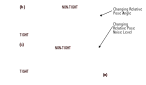
\includegraphics[width=\columnwidth]{figs/stereo_angle_study}
	\caption{Investigation of effect of pose interactions on tightness boundaries for two-pose localization with a stereo-camera model (parameters in body text). Boundaries indicates where the (smoothed) minimum \rev{ER } exceeds $ 10^{7}$ across 10 trials (without redundant constraints) and a diagram of the scenario is shown in (a). (b) shows the effect of observing the landmarks from a second pose at different vantage points, parameterized by the angle between poses. Noise level is fixed to 0.1 m and 0.1 rad. (c) Shows the effect of fixing the angle to 45 deg and varying the level of relative-pose noise (standard deviation in legend is equal for trans. and rot.).}
	\label{fig:stereo_angle}
\end{figure}

\subsubsection{Experiment in a Controlled Environment}

To assess tightness of stereo localization, we use the same setup as in Section \ref{sec:stereoslam_starry} randomly select 30 poses from the dataset and solve the SDP relaxation with and without redundant constraints. We add relative-pose measurements between subsequent poses based on the ground-truth data and perturb these measurements by a controlled amount of (isotropic) noise allowing to assess the effect of these additional measurements. 

Figure \ref{fig:d3_loc_box} shows the effect of adding redundant constraints on the \rev{ER } (tightness) of the localization problem. When there are no restrictions on the pose selection (Figure \ref{fig:d3_loc_box}(a)), it is clear that adding redundant constraints is required to obtain tightness for reasonable noise levels. When poses are restricted so that they observe at least 15 landmarks each (Figure \ref{fig:d3_loc_box}(b)), we see that, without redundant constraints, the problem is tight for higher levels of relative-pose noise and, with redundant constraints, the problem is tight across \emph{all noise levels}. This is consistent with the observations in Section \ref{sec:NoiseAnalysis}.


\begin{figure}[!b]
	\centering
	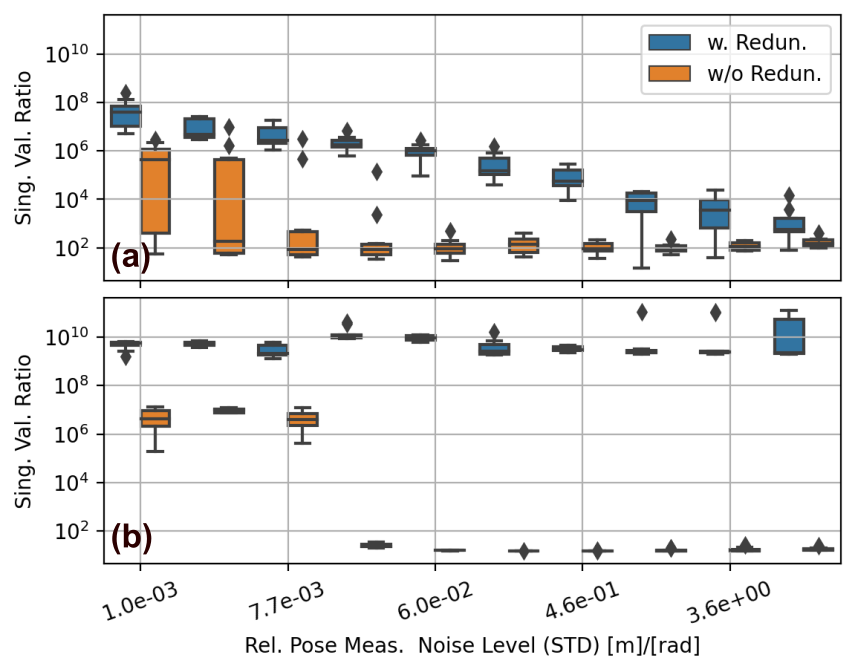
\includegraphics[width=\columnwidth]{figs/loc_box_plots}
	\caption{\rev{ER } results with and without redundant constraints for localization on random selections of 30 poses from the ``Starry Night'' dataset with relative-pose measurements between subsequent poses. 10 trials (random selection of poses) were performed at each noise level. (a) shows results when any pose can be selected, regardless of number of landmarks observed. (b) shows results when pose selection is restricted to poses that observe more than 15 landmarks.}
	\label{fig:d3_loc_box}
\end{figure}


\rev{\subsection{Other Metrics of Tightness}\label{App:otherMetrics}

In other works, it is sometimes the case that a `relative gap' is used as a metric for evaluating tightness of a convex relaxation. This gap is typically defined as follows:
\begin{equation*}
	\mbox{gap} = \frac{p(\bm{x}_r)-d^*}{1+d^*},
\end{equation*}
where $p(\bm{x}_r)$ represents the primal cost of the closest feasible, rank-1 solution (rounded solution) and $d^*$ represents the optimal SDP cost (equivalently, the dual cost). The one in the denominator keeps the metric stable when $d^*$ is low. 

In Figure~\ref{fig:compare_er_gap}, we compare this metric with the ER, our metric of choice throughout the paper. We note that the corresponding boundaries are very close, except when anistropicity is large. When redundant constraints were used, both metrics showed that the relaxation was tight for all parameter values.

\begin{figure}[!ht]
	\centering
	\includegraphics[width=\columnwidth]{figs/compare_er_gap.png}
	\caption{\rev{Comparison of ER and duality gap tightness boundary contours for the results in Figure~\ref{fig:ellipsoid_align} (without redundant constraints). The ER boundary corresponds to an ER of $1\times10^{-6}$ whereas the duality gap boundary corresponds to a relative gap of $1\times10^{-10}$.}}
	\label{fig:compare_er_gap}
\end{figure}
}
\subsection{Tightness Boundary Smoothing}\label{App:Smoothing}

As mentioned in the main body, we plot tightness boundaries based on the parameters for which the minimum \rev{ER } across all trials passes a threshold. \rev{These contours were plotted using the `contour' function from PyPlot. } However, it was initially found that the resulting contour plots were quite noisy and difficult to interpret even when the number of trials was increased considerably. To filter the data, the median of minimum \rev{ER } values was taken over an $N$-by-$N$ block in the parameter space (centered on a given parameter value) and the result was used to generate the smoothed contours. It was found that $N=7$ was sufficient to ensure adequate smoothing. A comparison of the contours on the raw minimum \rev{ER } data versus the filtered data is shown in Figure~\ref{fig:filter}, in which the data corresponds to the data in Figure~\ref{fig:ellipsoid_align} in the main text. 
\begin{figure}[!ht]
	\centering
	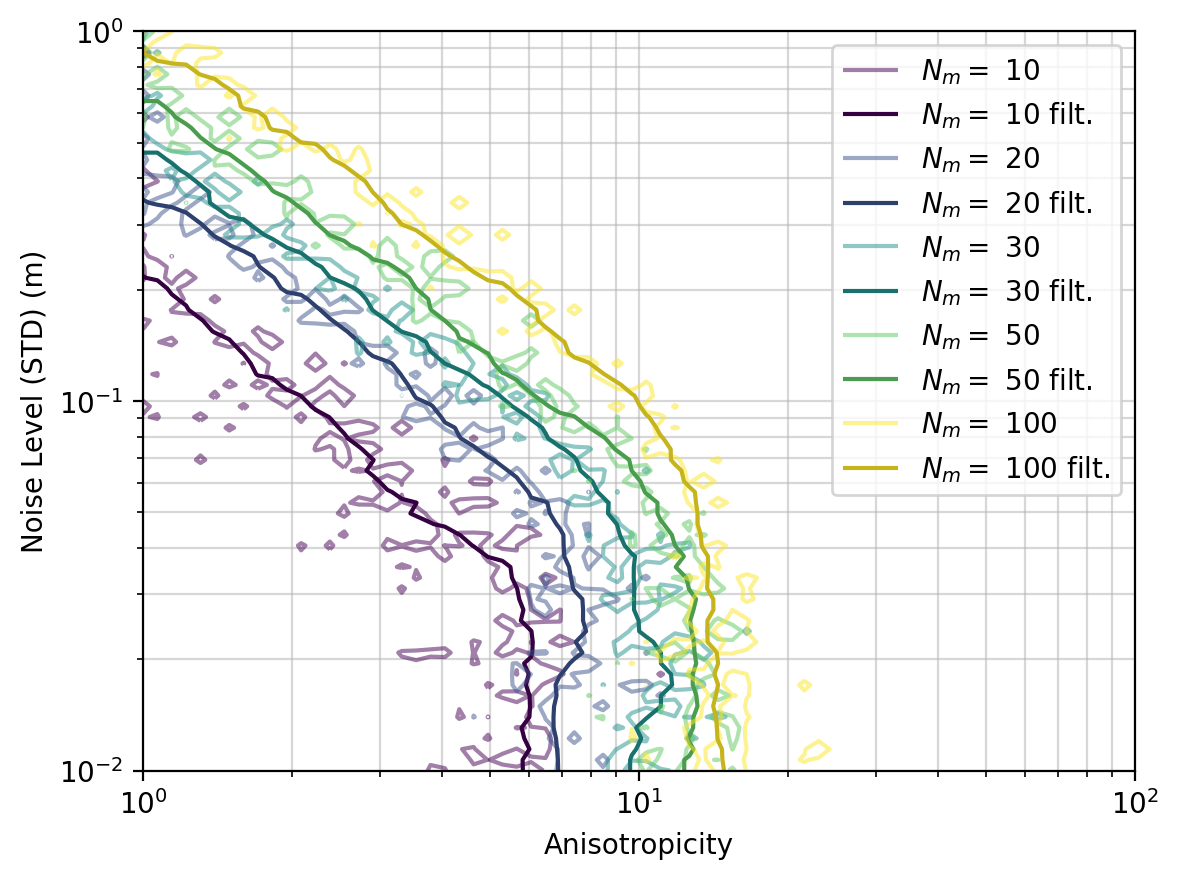
\includegraphics[width=\columnwidth]{figs/filter_compare}
	\caption{Comparison of tightness boundary contours with and without median filter for the results in Figure~\ref{fig:ellipsoid_align}. Darker contours (marked ``filt.'' in legend) represent the smoothed contours that were used in the body text.}
	\label{fig:filter}
\end{figure}


\subsection{Extended Results for Table~\ref{tbl:inthedark}}\label{App:inthedarkExt}


\begin{longtblr}[
	caption=Extended Results for Table~\ref{tbl:inthedark}
	]{llrrrrr}
	\hline
	{Map\\Run}& {Live\\Run}&Pipeline & {Avg. \\Time\\Per\\ Pose\\ (s)} & {Long.\\RMSE\\(m)} &  {Lat.\\RMSE\\(m)} &   {Head.\\RMSE\\(deg)} \\
	2 &       11 &         Baseline &    0.054 & 0.023 & 0.009 &  0.130 \\
	2 &       11 &           Global &    0.120 & 0.026 & 0.014 &  0.212 \\
	2 &       11 &            Local &    0.117 & 0.202 & 0.138 &  1.883 \\
	2 &       11 & {Local\\(filtered)} &    0.117 & 0.031 & 0.027 &  0.448 \\
	2 &       16 &         Baseline &    0.055 & 0.039 & 0.018 &  0.315 \\
	2 &       16 &           Global &    0.119 & 0.043 & 0.027 &  0.439 \\
	2 &       16 &            Local &    0.120 & 0.203 & 0.202 &  5.215 \\
	2 &       16 & {Local\\(filtered)} &    0.120 & 0.063 & 0.049 &  0.846 \\
	2 &       17 &         Baseline &    0.056 & 0.038 & 0.019 &  0.351 \\
	2 &       17 &           Global &    0.122 & 0.045 & 0.028 &  0.468 \\
	2 &       17 &            Local &    0.121 & 0.238 & 0.192 &  5.400 \\
	2 &       17 & {Local\\(filtered)} &    0.121 & 0.062 & 0.049 &  0.864 \\
	2 &       23 &         Baseline &    0.052 & 0.024 & 0.009 &  0.139 \\
	2 &       23 &           Global &    0.117 & 0.027 & 0.015 &  0.213 \\
	2 &       23 &            Local &    0.111 & 0.035 & 0.029 &  0.475 \\
	2 &       23 & {Local\\(filtered)} &    0.111 & 0.035 & 0.029 &  0.475 \\
	2 &       28 &         Baseline &    0.053 & 0.025 & 0.012 &  0.234 \\
	2 &       28 &           Global &    0.119 & 0.027 & 0.019 &  0.312 \\
	2 &       28 &            Local &    0.113 & 0.033 & 0.035 &  0.607 \\
	2 &       28 & {Local\\(filtered)} &    0.113 & 0.033 & 0.032 &  0.547 \\
	2 &       35 &         Baseline &    0.053 & 0.022 & 0.009 &  0.145 \\
	2 &       35 &           Global &    0.118 & 0.025 & 0.013 &  0.208 \\
	2 &       35 &            Local &    0.109 & 0.029 & 0.025 &  0.428 \\
	2 &       35 & {Local\\(filtered)} &    0.109 & 0.029 & 0.025 &  0.428 \\
	11 &       16 &         Baseline &    0.055 & 0.028 & 0.017 &  0.307 \\
	11 &       16 &           Global &    0.120 & 0.029 & 0.023 &  0.414 \\
	11 &       16 &            Local &    0.118 & 0.227 & 0.191 &  5.063 \\
	11 &       16 & {Local\\(filtered)} &    0.118 & 0.038 & 0.040 &  0.715 \\
	11 &       17 &         Baseline &    0.056 & 0.027 & 0.018 &  0.352 \\
	11 &       17 &           Global &    0.120 & 0.126 & 0.058 &  0.455 \\
	11 &       17 &            Local &    0.118 & 0.270 & 0.203 &  7.413 \\
	11 &       17 & {Local\\(filtered)} &    0.118 & 0.039 & 0.040 &  0.730 \\
	11 &       23 &         Baseline &    0.053 & 0.017 & 0.008 &  0.148 \\
	11 &       23 &           Global &    0.118 & 0.019 & 0.012 &  0.221 \\
	11 &       23 &            Local &    0.110 & 0.154 & 0.129 &  1.982 \\
	11 &       23 & {Local\\(filtered)} &    0.110 & 0.024 & 0.023 &  0.401 \\
	11 &       28 &         Baseline &    0.054 & 0.021 & 0.012 &  0.250 \\
	11 &       28 &           Global &    0.122 & 0.026 & 0.018 &  0.337 \\
	11 &       28 &            Local &    0.114 & 0.034 & 0.033 &  0.621 \\
	11 &       28 & {Local\\(filtered)} &    0.114 & 0.033 & 0.032 &  0.555 \\
	11 &       35 &         Baseline &    0.053 & 0.021 & 0.010 &  0.188 \\
	11 &       35 &           Global &    0.117 & 0.023 & 0.015 &  0.256 \\
	11 &       35 &            Local &    0.111 & 0.029 & 0.028 &  0.474 \\
	11 &       35 & {Local\\(filtered)} &    0.111 & 0.029 & 0.028 &  0.474 \\
	16 &       17 &         Baseline &    0.055 & 0.020 & 0.016 &  0.313 \\
	16 &       17 &           Global &    0.120 & 0.016 & 0.016 &  0.321 \\
	16 &       17 &            Local &    0.113 & 0.200 & 0.154 &  5.134 \\
	16 &       17 & {Local\\(filtered)} &    0.113 & 0.021 & 0.024 &  0.437 \\
	16 &       23 &         Baseline &    0.056 & 0.019 & 0.014 &  0.252 \\
	16 &       23 &           Global &    0.122 & 0.022 & 0.018 &  0.322 \\
	16 &       23 &            Local &    0.122 & 0.265 & 0.192 &  8.152 \\
	16 &       23 & {Local\\(filtered)} &    0.122 & 0.029 & 0.032 &  0.550 \\
	16 &       28 &         Baseline &    0.062 & 0.030 & 0.017 &  0.317 \\
	16 &       28 &           Global &    0.127 & 0.034 & 0.026 &  0.414 \\
	16 &       28 &            Local &    0.143 & 0.428 & 0.420 & 20.310 \\
	16 &       28 & {Local\\(filtered)} &    0.143 & 0.050 & 0.047 &  0.754 \\
	16 &       35 &         Baseline &    0.058 & 0.027 & 0.015 &  0.269 \\
	16 &       35 &           Global &    0.123 & 0.034 & 0.024 &  0.389 \\
	16 &       35 &            Local &    0.121 & 0.131 & 0.122 &  8.239 \\
	16 &       35 & {Local\\(filtered)} &    0.121 & 0.045 & 0.043 &  0.736 \\
	17 &       23 &         Baseline &    0.056 & 0.021 & 0.014 &  0.272 \\
	17 &       23 &           Global &    0.123 & 0.022 & 0.019 &  0.360 \\
	17 &       23 &            Local &    0.118 & 0.048 & 0.112 &  5.278 \\
	17 &       23 & {Local\\(filtered)} &    0.118 & 0.029 & 0.033 &  0.579 \\
	17 &       28 &         Baseline &    0.062 & 0.037 & 0.018 &  0.346 \\
	17 &       28 &           Global &    0.125 & 0.040 & 0.029 &  0.470 \\
	17 &       28 &            Local &    0.142 & 0.522 & 0.468 & 21.384 \\
	17 &       28 & {Local\\(filtered)} &    0.142 & 0.049 & 0.046 &  0.764 \\
	17 &       35 &         Baseline &    0.057 & 0.027 & 0.015 &  0.285 \\
	17 &       35 &           Global &    0.121 & 0.035 & 0.025 &  0.421 \\
	17 &       35 &            Local &    0.122 & 0.334 & 0.213 & 11.511 \\
	17 &       35 & {Local\\(filtered)} &    0.122 & 0.047 & 0.044 &  0.740 \\
	23 &       28 &         Baseline &    0.053 & 0.021 & 0.012 &  0.264 \\
	23 &       28 &           Global &    0.120 & 0.023 & 0.017 &  0.316 \\
	23 &       28 &            Local &    0.113 & 0.028 & 0.028 &  0.485 \\
	23 &       28 & {Local\\(filtered)} &    0.113 & 0.028 & 0.028 &  0.485 \\
	23 &       35 &         Baseline &    0.053 & 0.023 & 0.009 &  0.150 \\
	23 &       35 &           Global &    0.125 & 0.025 & 0.014 &  0.210 \\
	23 &       35 &            Local &    0.113 & 0.105 & 0.169 &  1.950 \\
	23 &       35 & {Local\\(filtered)} &    0.113 & 0.032 & 0.029 &  0.462 \\
	28 &       35 &         Baseline &    0.053 & 0.024 & 0.012 &  0.198 \\
	28 &       35 &           Global &    0.118 & 0.032 & 0.018 &  0.280 \\
	28 &       35 &            Local &    0.118 & 0.162 & 0.137 &  1.710 \\
	28 &       35 & {Local\\(filtered)} &    0.118 & 0.040 & 0.035 &  0.560 \\
	\hline
\end{longtblr}


\end{document}


